\documentclass[12pt]{article}

\usepackage{amsmath,amscd,amssymb,amsthm,enumerate,verbatim,palatino,parskip,graphicx}
\usepackage{tikz}

%\titleformat{\section}
%  {\newpage\rmfamily\Large\bfseries}{}{0em}{Lecture \thesection:~}
%\titlespacing*{\section}{0pt}{3.25ex plus 1ex minus .2ex}{1.5ex plus .2ex}

\usetikzlibrary{matrix,arrows,decorations.pathmorphing}
\usepackage{amsbsy,anysize}
\marginsize{2.3cm}{2.3cm}{2cm}{2.4cm}

\renewcommand\vec[1]{\ensuremath\boldsymbol{#1}}
\usepackage[T1]{fontenc}
\usepackage{hyperref}

\newcommand{\HRule}{\rule{\linewidth}{0.5mm}}

\newcommand{\dd}[2]{\frac{d #1}{d #2}}
\newcommand{\pd}[2]{\frac{\partial #1}{\partial #2}}
\newcommand{\m}{\mathcal}
\newcommand{\BB}{\mathbf}
\newcommand{\CC}{\mathbf{C}}
\newcommand{\RR}{\mathbf{R}}
\newcommand{\QQ}{\mathbf{Q}}
\newcommand{\PP}{\mathbf{P}}
\newcommand{\ZZ}{\mathbf{Z}}
\newcommand{\HH}{\mathbf{H}}
\newcommand{\KK}{\mathbf{K}}
\newcommand{\OP}{\operatorname}
\newcommand{\op}{\operatorname}
\newcommand{\into}{\hookrightarrow}
\newcommand{\Hom}{\mathrm{Hom}}
\newcommand{\End}{\OP{End}}
\newcommand{\ad}{\OP{ad}}
\newcommand{\Ad}{\OP{Ad}}
\newcommand{\Sym}{\OP{Sym}}
\renewcommand{\sl}{\mathfrak{sl}}
\renewcommand{\gg}{\mathfrak{g}}
\newcommand{\hh}{\mathfrak{h}}
\newcommand{\gl}{\mathfrak{gl}}
\newcommand{\id}{\mathrm{id}}
\newcommand{\diag}{\mathrm{diag}}
\newcommand{\Tr}{\mathrm{Tr}}
\newcommand{\kk}{\mathbf{k}}
\newcommand{\vrow}[2]{\left(\begin{array}{cc}#1 & #2\end{array}\right)}
\newcommand{\vcol}[2]{\left(\begin{array}{c}#1\\ #2\end{array}\right)}
\newcommand{\vrot}[3]{\left(\begin{array}{ccc}#1 & #2 & #3\end{array}\right)}
\newcommand{\vcot}[3]{\left(\begin{array}{c}#1\\ #2\\ #3\end{array}\right)}
\newcommand{\matr}[4]{\left(\begin{array}{cc}#1 & #2\\ #3 & #4\end{array}\right)}
\newcommand{\Diag}[3]{\left(\begin{array}{ccc}#1 & 0 & 0\\0 & #2 & 0\\0 & 0 & #3\end{array}\right)}
\newcommand{\mats}[4]{\left(\begin{array}{ccc}#1 & \cdots & #2\\ \vdots & \ddots & \vdots \\ #3 & \cdots & #4\end{array}\right)}
\newcommand{\matt}[9]{\left(\begin{array}{ccc}#1 & #2 & #3\\#4 & #5 & #6\\#7 & #8 & #9\end{array}\right)}
\newcommand{\MAT}[4]{\left(\begin{array}{ccc}#1 & \cdots & #2\\ \vdots & \ddots & \vdots\\ #3 & \cdots & #4\end{array}\right)}
\newcommand{\MATR}[9]{\left(\begin{array}{cccc}#1 & #2 & \cdots & #3\\ #4 & #5 &  & #6\\ \vdots & &\ddots &\vdots\\ #7 & #8 & \cdots & #9\\\end{array}\right)}

\setcounter{secnumdepth}{3}

\newtheorem{thm}{Theorem}[section]
\newtheorem{thmalpha}{Theorem}
\newtheorem{lma}[thm]{Lemma}
\newtheorem{lmaclub}[thm]{$\clubsuit$ Lemma}
\newtheorem{prp}[thm]{Proposition}
\newtheorem{cor}[thm]{Corollary}

\theoremstyle{definition}

\newtheorem{dfn}[thm]{Definition}
\newtheorem{exm}[thm]{Example}
\newtheorem{exmclub}[thm]{$\clubsuit$ Example}
\newtheorem{obs}[thm]{Observation}
\newtheorem*{clm}{Claim}

\newtheoremstyle{check}% name of the style to be used
  {}% measure of space to leave above the theorem. E.g.: 3pt
  {}% measure of space to leave below the theorem. E.g.: 3pt
  {}% name of font to use in the body of the theorem
  {}% measure of space to indent
  {\bf}% name of head font
  {!}% punctuation between head and body
  { }% space after theorem head; " " = normal interword space
  {}% manually specify head
\theoremstyle{check}
\newtheorem*{chk}{Check}

\theoremstyle{remark}
\newtheorem{rmk}[thm]{Remark}

\setcounter{tocdepth}{1}

\newtheoremstyle{TheoremNum}
    {\topsep}{\topsep}              %%% space between body and thm
    {\itshape}                      %%% Thm body font
    {}                              %%% Indent amount (empty = no indent)
    {\bfseries}                     %%% Thm head font
    {.}                             %%% Punctuation after thm head
    { }                             %%% Space after thm head
    {\thmname{#1}\thmnote{ \bfseries #3}}%%% Thm head spec
\theoremstyle{TheoremNum}

\begingroup 
\makeatletter 
\@for\theoremstyle:=definition,remark,plain,check,TheoremNum\do{% 
\expandafter\g@addto@macro\csname th@\theoremstyle\endcsname{% 
\addtolength\thm@preskip\parskip 
}% 
} 
\endgroup 

\renewcommand*{\thethmalpha}{\Alph{thmalpha}}

% Next bit redefines the proof environment so it's more like Arnold's book ``Mathematical methods of classical mechanics''.

\makeatletter \renewenvironment{proof}[1][\proofname]
{\par\pushQED{\qed}\normalfont\topsep6\p@\@plus6\p@\relax\begin{list}{}{\rightmargin=2em\leftmargin=2em}\item[\hskip\labelsep\bfseries#1\@addpunct{.}]\ignorespaces\footnotesize}{\popQED\end{list}\@endpefalse}
\makeatother

\usepackage{tikz}
\usetikzlibrary{arrows,decorations.markings}

% Structure of irreps of sl(2,C)

\newcommand{\sltwo}{\begin{center}
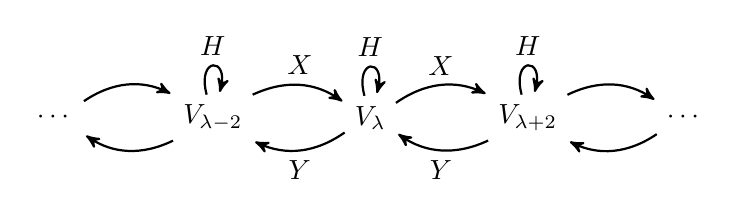
\begin{tikzpicture}[->,>=stealth',shorten >=1pt,auto,node distance=2cm,
  thick]

  \node (1) {$V_{\lambda}$};
  \node (2) [right of=1] {$V_{\lambda+2}$};
  \node (3) [left of=1] {$V_{\lambda-2}$};
  \node (4) [left of=3] {$\cdots$};
  \node (5) [right of=2] {$\cdots$};

  \path
    (1) edge [bend left] node [above] {$X$} (2)
        edge [bend left] node [below] {$Y$} (3)
        edge [loop above] node {$H$} (1)
    (2) edge [bend left] node [below] {$Y$} (1)
        edge [bend left] (5)
        edge [loop above] node {$H$} (2)
    (3) edge [bend left] node [above] {$X$} (1)
        edge [loop above] node {$H$} (3)
        edge [bend left] (4)
    (4) edge [bend left] (3)
    (5) edge [bend left] (2);
\end{tikzpicture}\end{center}}

% The roots of sl(3,C)

\newcommand{\slthree}{\begin{center}
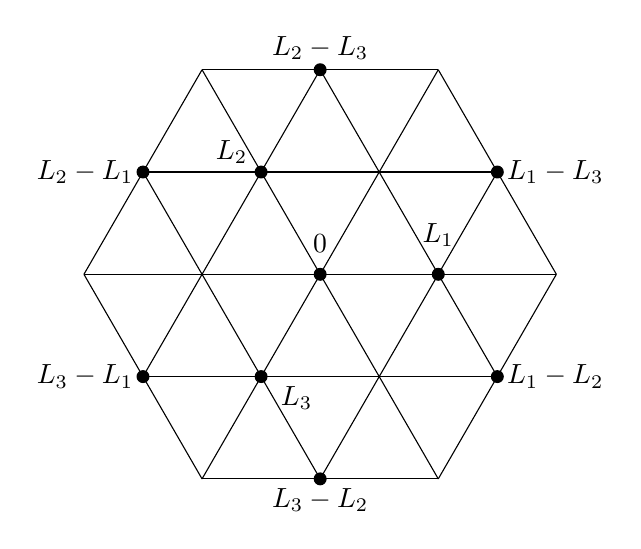
\begin{tikzpicture}[scale=1.5]
  \draw (240:2) -- (60:2);
  \draw (120:2) -- (300:2);
  \draw (60:2) -- (0:2);
  \draw (240:2) -- (180:2);
  \draw (180:2) -- (120:2);
  \draw (0:2) -- (300:2);
  \draw (120:2) -- (60:2);
  \draw (240:2) -- (300:2);
  \draw (180:2) -- (0:2);
  \draw (210:{2*sin{60}}) -- (330:{2*sin{60}});
  \draw (150:{2*sin{60}}) -- (30:{2*sin{60}});
  \draw (150:{2*sin{60}}) -- (270:{2*sin{60}});
  \draw (90:{2*sin{60}}) -- (330:{2*sin{60}});
  \draw (90:{2*sin{60}}) -- (210:{2*sin{60}});
  \draw (30:{2*sin{60}}) -- (270:{2*sin{60}});
  \draw[fill] (30:{2*sin{60}}) circle [radius=0.05];
  \draw[fill] (90:{2*sin{60}}) circle [radius=0.05];
  \draw[fill] (150:{2*sin{60}}) circle [radius=0.05];
  \draw[fill] (210:{2*sin{60}}) circle [radius=0.05];
  \draw[fill] (270:{2*sin{60}}) circle [radius=0.05];
  \draw[fill] (330:{2*sin{60}}) circle [radius=0.05];
  \draw[fill] (0,0) circle [radius=0.05];
  \draw[fill] (0:1) circle [radius=0.05];
  \draw[fill] (120:1) circle [radius=0.05];
  \draw[fill] (240:1) circle [radius=0.05];
  \node [above] at (0,0.1) {$0$};
  \node [above] at (1,0.15) {$L_1$};
  \node [below] at ({cos{120}-0.25},sin{120}+0.35) {$L_2$};
  \node [below] at ({cos{240}+0.3},sin{240}) {$L_3$};
  \node (1) [right] at (30:{2*sin{60}}) {$L_1-L_3$};
  \node (2) [above] at (90:{2*sin{60}}) {$L_2-L_3$};
  \node (3) [left] at (150:{2*sin{60}}) {$L_2-L_1$};
  \node (4) [left] at (210:{2*sin{60}}) {$L_3-L_1$};
  \node (5) [below] at (270:{2*sin{60}}) {$L_3-L_2$};
  \node (6) [right] at (330:{2*sin{60}}) {$L_1-L_2$};
\end{tikzpicture}\end{center}}

% And now for a diagram illustrating the adjoint action of root spaces on one another.

\newcommand{\sladj}{\begin{center}
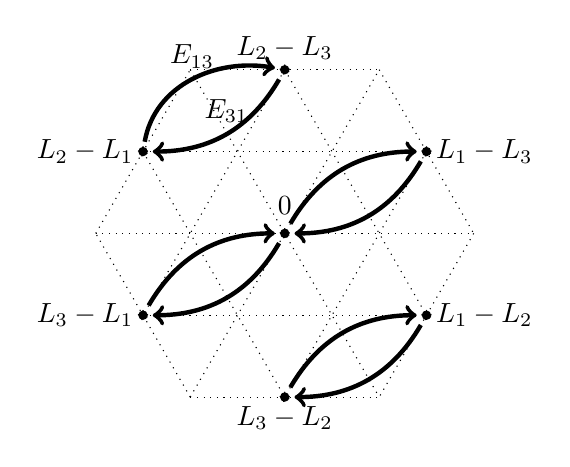
\begin{tikzpicture}[scale=1.2,dotted]
  \draw (240:2) -- (60:2);
  \draw (120:2) -- (300:2);
  \draw (60:2) -- (0:2);
  \draw (240:2) -- (180:2);
  \draw (180:2) -- (120:2);
  \draw (0:2) -- (300:2);
  \draw (120:2) -- (60:2);
  \draw (240:2) -- (300:2);
  \draw (180:2) -- (0:2);
  \draw (210:{2*sin{60}}) -- (330:{2*sin{60}});
  \draw (150:{2*sin{60}}) -- (30:{2*sin{60}});
  \draw (150:{2*sin{60}}) -- (270:{2*sin{60}});
  \draw (90:{2*sin{60}}) -- (330:{2*sin{60}});
  \draw (90:{2*sin{60}}) -- (210:{2*sin{60}});
  \draw (30:{2*sin{60}}) -- (270:{2*sin{60}});
  \draw[fill] (30:{2*sin{60}}) circle [radius=0.05];
  \draw[fill] (90:{2*sin{60}}) circle [radius=0.05];
  \draw[fill] (150:{2*sin{60}}) circle [radius=0.05];
  \draw[fill] (210:{2*sin{60}}) circle [radius=0.05];
  \draw[fill] (270:{2*sin{60}}) circle [radius=0.05];
  \draw[fill] (330:{2*sin{60}}) circle [radius=0.05];
  \draw[fill] (0,0) circle [radius=0.05];
  \node [above] at (0,0.1) {$0$};
  \node (0) at (0,0) {};
  \node [right] at (30:{2*sin{60}}) {$L_1-L_3$};
  \node (1) at (30:{2*sin{60}}) {};
  \node [above] at (90:{2*sin{60}}) {$L_2-L_3$};
  \node (2) at (90:{2*sin{60}}) {};
  \node [left] at (150:{2*sin{60}}) {$L_2-L_1$};
  \node (3) at (150:{2*sin{60}}) {};
  \node [left] at (210:{2*sin{60}}) {$L_3-L_1$};
  \node (4) at (210:{2*sin{60}}) {};
  \node [below] at (270:{2*sin{60}}) {$L_3-L_2$};
  \node (5) at (270:{2*sin{60}}) {};
  \node [right] at (330:{2*sin{60}}) {$L_1-L_2$};
  \node (6) at (330:{2*sin{60}}) {};
  \path[ultra thick,solid,->] 
  (3) edge [out=80,in=170] node [above] {$E_{13}$} (2)
  (2) edge [bend left] node [above] {$E_{31}$} (3)
  (4) edge [bend left] (0)
  (0) edge [bend left] (4)
  (0) edge [bend left] (1)
  (1) edge [bend left] (0)
  (5) edge [bend left] (6)
  (6) edge [bend left] (5);
\end{tikzpicture}
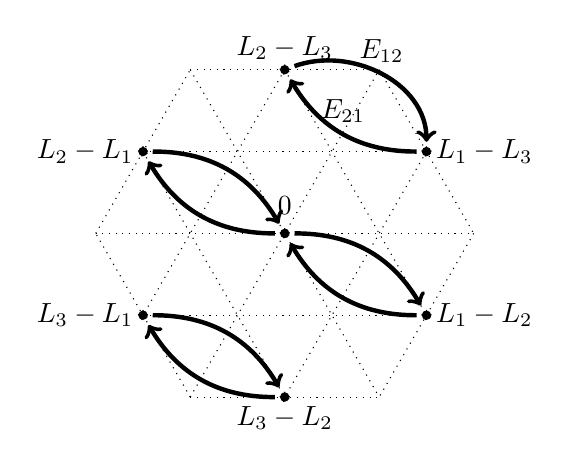
\begin{tikzpicture}[scale=1.2,dotted]
  \draw (240:2) -- (60:2);
  \draw (120:2) -- (300:2);
  \draw (60:2) -- (0:2);
  \draw (240:2) -- (180:2);
  \draw (180:2) -- (120:2);
  \draw (0:2) -- (300:2);
  \draw (120:2) -- (60:2);
  \draw (240:2) -- (300:2);
  \draw (180:2) -- (0:2);
  \draw (210:{2*sin{60}}) -- (330:{2*sin{60}});
  \draw (150:{2*sin{60}}) -- (30:{2*sin{60}});
  \draw (150:{2*sin{60}}) -- (270:{2*sin{60}});
  \draw (90:{2*sin{60}}) -- (330:{2*sin{60}});
  \draw (90:{2*sin{60}}) -- (210:{2*sin{60}});
  \draw (30:{2*sin{60}}) -- (270:{2*sin{60}});
  \draw[fill] (30:{2*sin{60}}) circle [radius=0.05];
  \draw[fill] (90:{2*sin{60}}) circle [radius=0.05];
  \draw[fill] (150:{2*sin{60}}) circle [radius=0.05];
  \draw[fill] (210:{2*sin{60}}) circle [radius=0.05];
  \draw[fill] (270:{2*sin{60}}) circle [radius=0.05];
  \draw[fill] (330:{2*sin{60}}) circle [radius=0.05];
  \draw[fill] (0,0) circle [radius=0.05];
  \node [above] at (0,0.1) {$0$};
  \node (0) at (0,0) {};
  \node [right] at (30:{2*sin{60}}) {$L_1-L_3$};
  \node (1) at (30:{2*sin{60}}) {};
  \node [above] at (90:{2*sin{60}}) {$L_2-L_3$};
  \node (2) at (90:{2*sin{60}}) {};
  \node [left] at (150:{2*sin{60}}) {$L_2-L_1$};
  \node (3) at (150:{2*sin{60}}) {};
  \node [left] at (210:{2*sin{60}}) {$L_3-L_1$};
  \node (4) at (210:{2*sin{60}}) {};
  \node [below] at (270:{2*sin{60}}) {$L_3-L_2$};
  \node (5) at (270:{2*sin{60}}) {};
  \node [right] at (330:{2*sin{60}}) {$L_1-L_2$};
  \node (6) at (330:{2*sin{60}}) {};
  \path[ultra thick,solid,->] 
  (2) edge [in=90,out=20] node [above] {$E_{12}$} (1)
  (1) edge [bend left] node [above] {$E_{21}$} (2)
  (3) edge [bend left] (0)
  (0) edge [bend left] (3)
  (0) edge [bend left] (6)
  (6) edge [bend left] (0)
  (4) edge [bend left] (5)
  (5) edge [bend left] (4);
\end{tikzpicture}
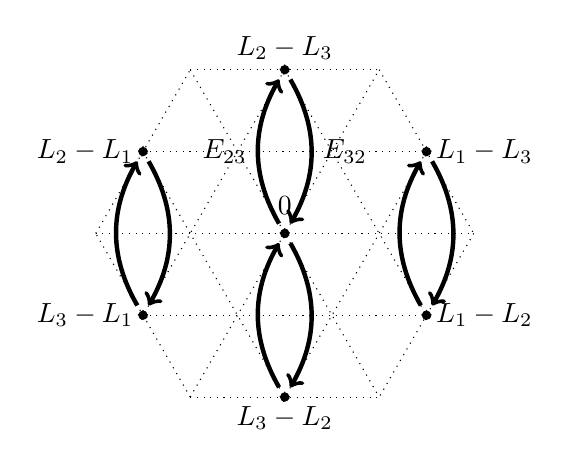
\begin{tikzpicture}[scale=1.2,dotted]
  \draw (240:2) -- (60:2);
  \draw (120:2) -- (300:2);
  \draw (60:2) -- (0:2);
  \draw (240:2) -- (180:2);
  \draw (180:2) -- (120:2);
  \draw (0:2) -- (300:2);
  \draw (120:2) -- (60:2);
  \draw (240:2) -- (300:2);
  \draw (180:2) -- (0:2);
  \draw (210:{2*sin{60}}) -- (330:{2*sin{60}});
  \draw (150:{2*sin{60}}) -- (30:{2*sin{60}});
  \draw (150:{2*sin{60}}) -- (270:{2*sin{60}});
  \draw (90:{2*sin{60}}) -- (330:{2*sin{60}});
  \draw (90:{2*sin{60}}) -- (210:{2*sin{60}});
  \draw (30:{2*sin{60}}) -- (270:{2*sin{60}});
  \draw[fill] (30:{2*sin{60}}) circle [radius=0.05];
  \draw[fill] (90:{2*sin{60}}) circle [radius=0.05];
  \draw[fill] (150:{2*sin{60}}) circle [radius=0.05];
  \draw[fill] (210:{2*sin{60}}) circle [radius=0.05];
  \draw[fill] (270:{2*sin{60}}) circle [radius=0.05];
  \draw[fill] (330:{2*sin{60}}) circle [radius=0.05];
  \draw[fill] (0,0) circle [radius=0.05];
  \node [above] at (0,0.1) {$0$};
  \node (0) at (0,0) {};
  \node [right] at (30:{2*sin{60}}) {$L_1-L_3$};
  \node (1) at (30:{2*sin{60}}) {};
  \node [above] at (90:{2*sin{60}}) {$L_2-L_3$};
  \node (2) at (90:{2*sin{60}}) {};
  \node [left] at (150:{2*sin{60}}) {$L_2-L_1$};
  \node (3) at (150:{2*sin{60}}) {};
  \node [left] at (210:{2*sin{60}}) {$L_3-L_1$};
  \node (4) at (210:{2*sin{60}}) {};
  \node [below] at (270:{2*sin{60}}) {$L_3-L_2$};
  \node (5) at (270:{2*sin{60}}) {};
  \node [right] at (330:{2*sin{60}}) {$L_1-L_2$};
  \node (6) at (330:{2*sin{60}}) {};
  \path[ultra thick,solid,->] 
  (0) edge [bend left] node [left] {$E_{23}$} (2)
  (2) edge [bend left] node [right] {$E_{32}$} (0)
  (0) edge [bend left] (5)
  (5) edge [bend left] (0)
  (1) edge [bend left] (6)
  (6) edge [bend left] (1)
  (4) edge [bend left] (3)
  (3) edge [bend left] (4);
\end{tikzpicture}\end{center}}

\newcommand{\slhwv}{\begin{center}
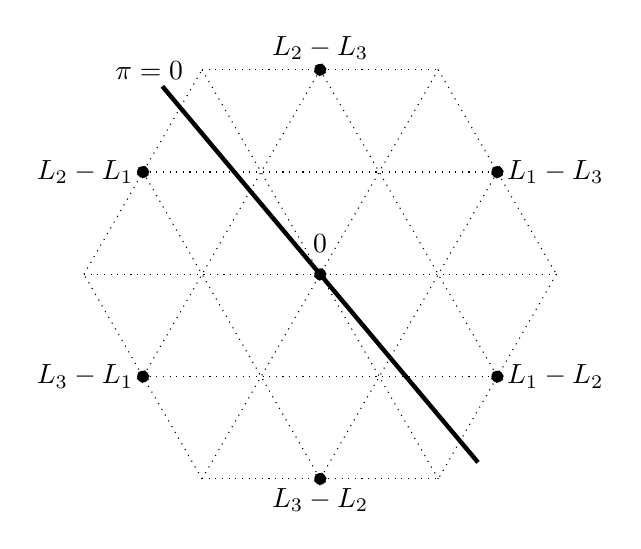
\begin{tikzpicture}[scale=1.5,dotted]
  \draw (240:2) -- (60:2);
  \draw (120:2) -- (300:2);
  \draw (60:2) -- (0:2);
  \draw (240:2) -- (180:2);
  \draw (180:2) -- (120:2);
  \draw (0:2) -- (300:2);
  \draw (120:2) -- (60:2);
  \draw (240:2) -- (300:2);
  \draw (180:2) -- (0:2);
  \draw (210:{2*sin{60}}) -- (330:{2*sin{60}});
  \draw (150:{2*sin{60}}) -- (30:{2*sin{60}});
  \draw (150:{2*sin{60}}) -- (270:{2*sin{60}});
  \draw (90:{2*sin{60}}) -- (330:{2*sin{60}});
  \draw (90:{2*sin{60}}) -- (210:{2*sin{60}});
  \draw (30:{2*sin{60}}) -- (270:{2*sin{60}});
  \draw[fill] (30:{2*sin{60}}) circle [radius=0.05];
  \draw[fill] (90:{2*sin{60}}) circle [radius=0.05];
  \draw[fill] (150:{2*sin{60}}) circle [radius=0.05];
  \draw[fill] (210:{2*sin{60}}) circle [radius=0.05];
  \draw[fill] (270:{2*sin{60}}) circle [radius=0.05];
  \draw[fill] (330:{2*sin{60}}) circle [radius=0.05];
  \draw[fill] (0,0) circle [radius=0.05];
  \node [above] at (0,0.1) {$0$};
  \node (0) at (0,0) {};
  \node [right] at (30:{2*sin{60}}) {$L_1-L_3$};
  \node (1) at (30:{2*sin{60}}) {};
  \node [above] at (90:{2*sin{60}}) {$L_2-L_3$};
  \node (2) at (90:{2*sin{60}}) {};
  \node [left] at (150:{2*sin{60}}) {$L_2-L_1$};
  \node (3) at (150:{2*sin{60}}) {};
  \node [left] at (210:{2*sin{60}}) {$L_3-L_1$};
  \node (4) at (210:{2*sin{60}}) {};
  \node [below] at (270:{2*sin{60}}) {$L_3-L_2$};
  \node (5) at (270:{2*sin{60}}) {};
  \node [right] at (330:{2*sin{60}}) {$L_1-L_2$};
  \node (6) at (330:{2*sin{60}}) {};
  \draw[ultra thick,solid] (310:{2.4*sin{60}}) -- (130:{2.4*sin{60}});
  \node at (130:{2.6*sin{60}}) {$\pi=0$};
\end{tikzpicture}\end{center}}

\newcommand{\sltritant}{\begin{center}
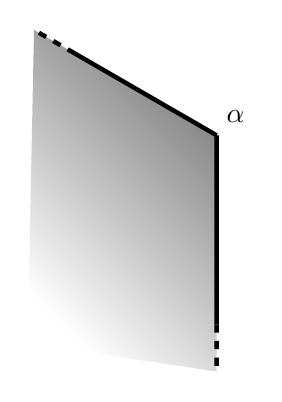
\begin{tikzpicture}[scale=1.2]
  \node at (0.2,0.2) {$\alpha$};
  \shade [shading angle=-45]
      (0,-2.5) -- (0,0) -- (150:2.23205080757) -- (-2,-2.2) -- cycle;
  \draw [ultra thick]
     (0,0) -- (0,-2)
     (0,0) -- (150:1.73205080757);
  \draw [ultra thick,dashed]
     (0,-2) -- (0,-2.5)
     (150:1.73205080757) -- (150:2.23205080757);
\end{tikzpicture}
\end{center}}

% The weight diagram for the standard representation of SU(3)

\newcommand{\slthreestd}{\begin{center}
\begin{tikzpicture}[scale=2,dotted]
  \draw (-1,0) -- (1,0);
  \draw (120:1) -- (60:1);
  \draw (240:1) -- (300:1);
  \draw (240:1) -- (60:1);
  \draw (120:1) -- (300:1);
  \draw (120:1) -- (180:1);
  \draw (180:1) -- (240:1);
  \draw (300:1) -- (1,0);
  \draw (1,0) -- (60:1);
  \draw[fill] (120:1) circle [radius=0.05];
  \draw[fill] (240:1) circle [radius=0.05];
  \draw[fill] (1,0) circle [radius=0.05];
  \node [above] at (0,0.1) {$0$};
  \node [above] at (1,0.15) {$L_1$};
  \node [below] at ({cos{120}-0.25},sin{120}+0.35) {$L_2$};
  \node [below] at ({cos{240}+0.3},sin{240}) {$L_3$};
\end{tikzpicture}\end{center}}

\newcommand{\slthreedual}{\begin{center}
\begin{tikzpicture}[scale=2,dotted]
  \draw (-1,0) -- (1,0);
  \draw (120:1) -- (60:1);
  \draw (240:1) -- (300:1);
  \draw (240:1) -- (60:1);
  \draw (120:1) -- (300:1);
  \draw (120:1) -- (180:1);
  \draw (180:1) -- (240:1);
  \draw (300:1) -- (1,0);
  \draw (1,0) -- (60:1);
  \draw[fill] (60:1) circle [radius=0.05];
  \draw[fill] (300:1) circle [radius=0.05];
  \draw[fill] (-1,0) circle [radius=0.05];
  \node [above] at (0,0.1) {$0$};
  \node at (-1.3,0) {$-L_1$};
  \node [below] at ({cos{60}+0.25},sin{60}+0.35) {$-L_2$};
  \node [below] at ({cos{300}+0.3},sin{300}) {$-L_3$};
\end{tikzpicture}\end{center}}

% The root diagram again, without L_1, L_2, L_3

\newcommand{\sladjwt}{\begin{center}
\begin{tikzpicture}[scale=1.5,dotted,bigger node/.style={fill=black,circle,draw,text=white,inner sep=1pt,font=\boldmath}]
  \draw (240:2) -- (60:2);
  \draw (120:2) -- (300:2);
  \draw (60:2) -- (0:2);
  \draw (240:2) -- (180:2);
  \draw (180:2) -- (120:2);
  \draw (0:2) -- (300:2);
  \draw (120:2) -- (60:2);
  \draw (240:2) -- (300:2);
  \draw (180:2) -- (0:2);
  \draw (210:{2*sin{60}}) -- (330:{2*sin{60}});
  \draw (150:{2*sin{60}}) -- (30:{2*sin{60}});
  \draw (150:{2*sin{60}}) -- (270:{2*sin{60}});
  \draw (90:{2*sin{60}}) -- (330:{2*sin{60}});
  \draw (90:{2*sin{60}}) -- (210:{2*sin{60}});
  \draw (30:{2*sin{60}}) -- (270:{2*sin{60}});
  \draw[fill] (30:{2*sin{60}}) circle [radius=0.05];
  \draw[fill] (90:{2*sin{60}}) circle [radius=0.05];
  \draw[fill] (150:{2*sin{60}}) circle [radius=0.05];
  \draw[fill] (210:{2*sin{60}}) circle [radius=0.05];
  \draw[fill] (270:{2*sin{60}}) circle [radius=0.05];
  \draw[fill] (330:{2*sin{60}}) circle [radius=0.05];
  \draw[fill] (0,0) circle [radius=0.05];
  \node [above] at (0,0.3) {$0$};
  \node[bigger node] (0) at (0,0) {2};
  \node [right] at (30:{2*sin{60}}) {$L_1-L_3$};
  \node (1) at (30:{2*sin{60}}) {};
  \node [above] at (90:{2*sin{60}}) {$L_2-L_3$};
  \node (2) at (90:{2*sin{60}}) {};
  \node [left] at (150:{2*sin{60}}) {$L_2-L_1$};
  \node (3) at (150:{2*sin{60}}) {};
  \node [left] at (210:{2*sin{60}}) {$L_3-L_1$};
  \node (4) at (210:{2*sin{60}}) {};
  \node [below] at (270:{2*sin{60}}) {$L_3-L_2$};
  \node (5) at (270:{2*sin{60}}) {};
  \node [right] at (330:{2*sin{60}}) {$L_1-L_2$};
  \node (6) at (330:{2*sin{60}}) {};
\end{tikzpicture}\end{center}}

% Weight diagram for the tensor square of the standard representation of SU(3)

\newcommand{\sltensq}[1]{\begin{center}
\begin{tikzpicture}[scale=#1*1.5,dotted,bigger node/.style={fill=black,circle,draw,text=white,inner sep=1pt,font=\boldmath}]
  \draw (-1,0) -- (2,0);
  \draw (120:2) -- (300:2);
  \draw (240:2) -- (60:2);
  \draw (120:2) -- (60:2);
  \draw (240:2) -- (300:2);
  \draw (60:2) -- (2,0);
  \draw (300:2) -- (2,0);
  \draw (0,{2*sin{60}}) -- (-1,0);
  \draw (0,{-2*sin{60}}) -- (-1,0);
  \draw (0,{2*sin{60}}) -- ({1+cos{60}},-{sin{60}});
  \draw (0,{-2*sin{60}}) -- ({1+cos{60}},{sin{60}});
  \draw (-1,{sin{60}}) -- ({1+cos{60}},{sin{60}});
  \draw (-1,{-sin{60}}) -- ({1+cos{60}},{-sin{60}});
  \draw[fill] (120:2) circle [radius=0.05];
  \draw[fill] (240:2) circle [radius=0.05];
  \draw[fill] (2,0) circle [radius=0.05];
  \node[bigger node] at (60:1) {2};
  \node[bigger node] at (300:1) {2};
  \node[bigger node] at (-1,0) {2};
  \node at (0,0) {$0$};
\end{tikzpicture}\end{center}}

\newcommand{\slsymsq}[1]{\begin{center}
\begin{tikzpicture}[scale=#1*1.5,dotted]
  \draw (-1,0) -- (2,0);
  \draw (120:2) -- (300:2);
  \draw (240:2) -- (60:2);
  \draw (120:2) -- (60:2);
  \draw (240:2) -- (300:2);
  \draw (60:2) -- (2,0);
  \draw (300:2) -- (2,0);
  \draw (0,{2*sin{60}}) -- (-1,0);
  \draw (0,{-2*sin{60}}) -- (-1,0);
  \draw (0,{2*sin{60}}) -- ({1+cos{60}},-{sin{60}});
  \draw (0,{-2*sin{60}}) -- ({1+cos{60}},{sin{60}});
  \draw (-1,{sin{60}}) -- ({1+cos{60}},{sin{60}});
  \draw (-1,{-sin{60}}) -- ({1+cos{60}},{-sin{60}});
  \draw[fill] (120:2) circle [radius=0.05];
  \draw[fill] (240:2) circle [radius=0.05];
  \draw[fill] (2,0) circle [radius=0.05];
  \draw[fill] (60:1) circle [radius=0.05];
  \draw[fill] (300:1) circle [radius=0.05];
  \draw[fill] (-1,0) circle [radius=0.05];
  \node at (0,0) {$0$};
\end{tikzpicture}\end{center}}

\newcommand{\slbeast}{\begin{center}
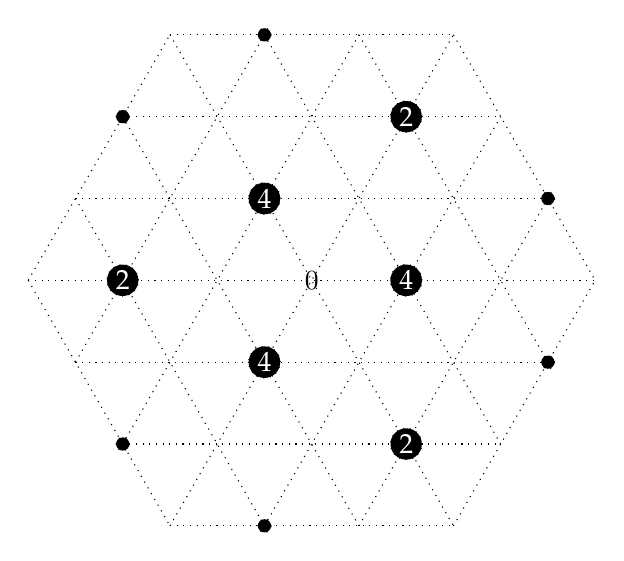
\begin{tikzpicture}[scale=1.2,dotted,bigger node/.style={fill=black,circle,draw,text=white,inner sep=1pt,font=\boldmath}]
  \draw (-3,0) -- (3,0);
  \draw (240:3) -- (60:3);
  \draw (120:3) -- (300:3);
  \draw (-3,0) -- (120:3);
  \draw (-3,0) -- (240:3);
  \draw (120:3) -- (60:3);
  \draw (240:3) -- (300:3);
  \draw (300:3) -- (3,0);
  \draw (60:3) -- (3,0);
  \draw (-2,{2*sin{60}}) -- (2,{2*sin{60}});
  \draw ({-2-cos{60}},{sin{60}}) -- ({2+cos{60}},{sin{60}});
  \draw (-2,{-2*sin{60}}) -- (2,{-2*sin{60}});
  \draw ({-2-cos{60}},{-sin{60}}) -- ({2+cos{60}},{-sin{60}});
  \draw (-2,{2*sin{60}}) -- (2,{2*sin{60}});
  \draw ({-2-cos{60}},{sin{60}}) -- ({-cos{60}},{-3*sin{60}});
  \draw ({-2},{2*sin{60}}) -- ({cos{60}},{-3*sin{60}});
  \draw ({-cos{60}},{3*sin{60}}) -- ({2},{-2*sin{60}});
  \draw ({cos{60}},{3*sin{60}}) -- ({2+cos{60}},{-sin{60}});
  \draw ({cos{60}},{-3*sin{60}}) -- ({2+cos{60}},{sin{60}});
  \draw ({-cos{60}},{-3*sin{60}}) -- ({2},{2*sin{60}});
  \draw ({-2},{-2*sin{60}}) -- ({cos{60}},{3*sin{60}});
  \draw ({-2-cos{60}},{-sin{60}}) -- ({-cos{60}},{3*sin{60}});
  \draw[fill] ({-cos{60}},{3*sin{60}}) circle [radius=0.07];
  \draw[fill] (-2,{2*sin{60}}) circle [radius=0.07];
  \node[bigger node] at (-2,0) {2};
  \draw[fill] ({-cos{60}},{-3*sin{60}}) circle [radius=0.07];
  \draw[fill] (-2,{-2*sin{60}}) circle [radius=0.07];
  \node[bigger node] at (1,{2*sin{60}}) {2};
  \node[bigger node] at (1,{-2*sin{60}}) {2};
  \draw[fill] (2.5,{sin{60}}) circle [radius=0.07];
  \draw[fill] (2.5,{-sin{60}}) circle [radius=0.07];
  \node[bigger node] at (120:1) {4};
  \node[bigger node] at (240:1) {4};
  \node[bigger node] at (0:1) {4};
  \node at (0,0) {$0$};
\end{tikzpicture}\end{center}}

\newcommand{\sltwoone}{\begin{center}
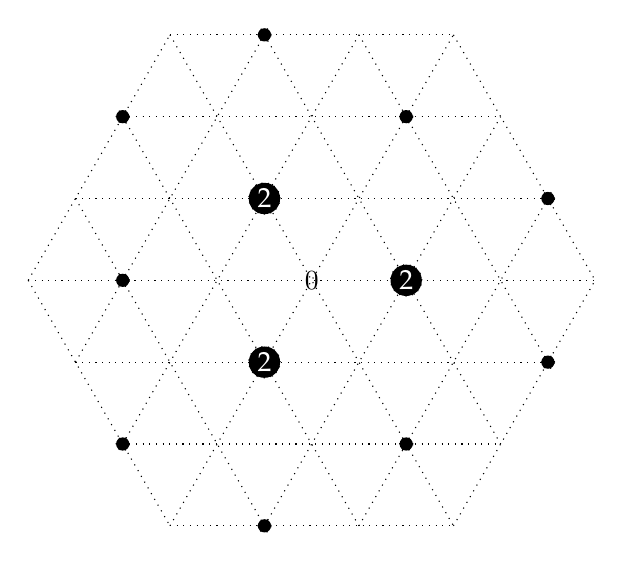
\begin{tikzpicture}[scale=1.2,dotted,bigger node/.style={fill=black,circle,draw,text=white,inner sep=1pt,font=\boldmath}]
  \draw (-3,0) -- (3,0);
  \draw (240:3) -- (60:3);
  \draw (120:3) -- (300:3);
  \draw (-3,0) -- (120:3);
  \draw (-3,0) -- (240:3);
  \draw (120:3) -- (60:3);
  \draw (240:3) -- (300:3);
  \draw (300:3) -- (3,0);
  \draw (60:3) -- (3,0);
  \draw (-2,{2*sin{60}}) -- (2,{2*sin{60}});
  \draw ({-2-cos{60}},{sin{60}}) -- ({2+cos{60}},{sin{60}});
  \draw (-2,{-2*sin{60}}) -- (2,{-2*sin{60}});
  \draw ({-2-cos{60}},{-sin{60}}) -- ({2+cos{60}},{-sin{60}});
  \draw (-2,{2*sin{60}}) -- (2,{2*sin{60}});
  \draw ({-2-cos{60}},{sin{60}}) -- ({-cos{60}},{-3*sin{60}});
  \draw ({-2},{2*sin{60}}) -- ({cos{60}},{-3*sin{60}});
  \draw ({-cos{60}},{3*sin{60}}) -- ({2},{-2*sin{60}});
  \draw ({cos{60}},{3*sin{60}}) -- ({2+cos{60}},{-sin{60}});
  \draw ({cos{60}},{-3*sin{60}}) -- ({2+cos{60}},{sin{60}});
  \draw ({-cos{60}},{-3*sin{60}}) -- ({2},{2*sin{60}});
  \draw ({-2},{-2*sin{60}}) -- ({cos{60}},{3*sin{60}});
  \draw ({-2-cos{60}},{-sin{60}}) -- ({-cos{60}},{3*sin{60}});
  \draw[fill] ({-cos{60}},{3*sin{60}}) circle [radius=0.07];
  \draw[fill] (-2,{2*sin{60}}) circle [radius=0.07];
  \draw[fill] (-2,0) circle [radius=0.07];
  \draw[fill] ({-cos{60}},{-3*sin{60}}) circle [radius=0.07];
  \draw[fill] (-2,{-2*sin{60}}) circle [radius=0.07];
  \draw[fill] (1,{2*sin{60}}) circle [radius=0.07];
  \draw[fill] (1,{-2*sin{60}}) circle [radius=0.07];
  \draw[fill] (2.5,{sin{60}}) circle [radius=0.07];
  \draw[fill] (2.5,{-sin{60}}) circle [radius=0.07];
  \node[bigger node] at (120:1) {2};
  \node[bigger node] at (240:1) {2};
  \node[bigger node] at (0:1) {2};
  \node at (0,0) {$0$};
\end{tikzpicture}\end{center}}

\newcommand{\slstdtensordual}{\begin{center}
\begin{tikzpicture}[scale=1.5,dotted,bigger node/.style={fill=black,circle,draw,text=white,inner sep=1pt,font=\boldmath}]
  \draw (240:2) -- (60:2);
  \draw (120:2) -- (300:2);
  \draw (60:2) -- (0:2);
  \draw (240:2) -- (180:2);
  \draw (180:2) -- (120:2);
  \draw (0:2) -- (300:2);
  \draw (120:2) -- (60:2);
  \draw (240:2) -- (300:2);
  \draw (180:2) -- (0:2);
  \draw (210:{2*sin{60}}) -- (330:{2*sin{60}});
  \draw (150:{2*sin{60}}) -- (30:{2*sin{60}});
  \draw (150:{2*sin{60}}) -- (270:{2*sin{60}});
  \draw (90:{2*sin{60}}) -- (330:{2*sin{60}});
  \draw (90:{2*sin{60}}) -- (210:{2*sin{60}});
  \draw (30:{2*sin{60}}) -- (270:{2*sin{60}});
  \draw[fill] (30:{2*sin{60}}) circle [radius=0.05];
  \draw[fill] (90:{2*sin{60}}) circle [radius=0.05];
  \draw[fill] (150:{2*sin{60}}) circle [radius=0.05];
  \draw[fill] (210:{2*sin{60}}) circle [radius=0.05];
  \draw[fill] (270:{2*sin{60}}) circle [radius=0.05];
  \draw[fill] (330:{2*sin{60}}) circle [radius=0.05];
  \draw[fill] (0,0) circle [radius=0.05];
  \node [above] at (0,0.3) {$0$};
  \node[bigger node] (0) at (0,0) {3};
  \node [right] at (30:{2*sin{60}}) {$L_1-L_3$};
  \node (1) at (30:{2*sin{60}}) {};
  \node [above] at (90:{2*sin{60}}) {$L_2-L_3$};
  \node (2) at (90:{2*sin{60}}) {};
  \node [left] at (150:{2*sin{60}}) {$L_2-L_1$};
  \node (3) at (150:{2*sin{60}}) {};
  \node [left] at (210:{2*sin{60}}) {$L_3-L_1$};
  \node (4) at (210:{2*sin{60}}) {};
  \node [below] at (270:{2*sin{60}}) {$L_3-L_2$};
  \node (5) at (270:{2*sin{60}}) {};
  \node [right] at (330:{2*sin{60}}) {$L_1-L_2$};
  \node (6) at (330:{2*sin{60}}) {};
\end{tikzpicture}\end{center}}

\newcommand{\meson}{\begin{center}
\begin{tikzpicture}[scale=1.5,dotted]
  \draw (240:2) -- (60:2);
  \draw (120:2) -- (300:2);
  \draw (60:2) -- (0:2);
  \draw (240:2) -- (180:2);
  \draw (180:2) -- (120:2);
  \draw (0:2) -- (300:2);
  \draw (120:2) -- (60:2);
  \draw (240:2) -- (300:2);
  \draw (180:2) -- (0:2);
  \draw (210:{2*sin{60}}) -- (330:{2*sin{60}});
  \draw (150:{2*sin{60}}) -- (30:{2*sin{60}});
  \draw (150:{2*sin{60}}) -- (270:{2*sin{60}});
  \draw (90:{2*sin{60}}) -- (330:{2*sin{60}});
  \draw (90:{2*sin{60}}) -- (210:{2*sin{60}});
  \draw (30:{2*sin{60}}) -- (270:{2*sin{60}});
  \draw[fill] (30:{2*sin{60}}) circle [radius=0.05];
  \draw[fill] (90:{2*sin{60}}) circle [radius=0.05];
  \draw[fill] (150:{2*sin{60}}) circle [radius=0.05];
  \draw[fill] (210:{2*sin{60}}) circle [radius=0.05];
  \draw[fill] (270:{2*sin{60}}) circle [radius=0.05];
  \draw[fill] (330:{2*sin{60}}) circle [radius=0.05];
  \draw[fill] (0,0) circle [radius=0.05];
  \node [above] at (0,0.1) {$0$};
  \node (0) at (0,0) {};
  \node [right] at (30:{2*sin{60}}) {$u\bar{s}=K^+$};
  \node (1) at (30:{2*sin{60}}) {};
  \node [above] at (90:{2*sin{60}}) {$d\bar{s}=K^0$};
  \node (2) at (90:{2*sin{60}}) {};
  \node [left] at (150:{2*sin{60}}) {$d\bar{u}=\pi^-$};
  \node (3) at (150:{2*sin{60}}) {};
  \node [left] at (210:{2*sin{60}}) {$s\bar{u}=K^-$};
  \node (4) at (210:{2*sin{60}}) {};
  \node [below] at (270:{2*sin{60}}) {$s\bar{d}=\bar{K}^0$};
  \node (5) at (270:{2*sin{60}}) {};
  \node [right] at (330:{2*sin{60}}) {$u\bar{d}=\pi^+$};
  \node (6) at (330:{2*sin{60}}) {};
\end{tikzpicture}\end{center}}

\newcommand{\baryon}{\begin{center}
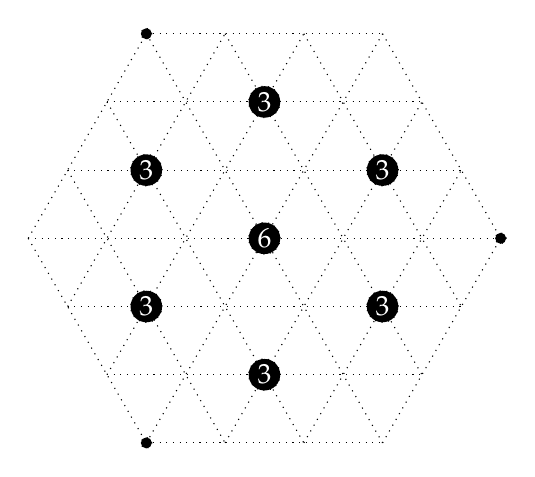
\begin{tikzpicture}[dotted,every node/.style={fill=black,circle,draw,text=white,inner sep=1pt,font=\boldmath}]
  \draw (-3,0) -- (3,0);
  \draw (240:3) -- (60:3);
  \draw (120:3) -- (300:3);
  \draw (-3,0) -- (120:3);
  \draw (-3,0) -- (240:3);
  \draw (120:3) -- (60:3);
  \draw (240:3) -- (300:3);
  \draw (300:3) -- (3,0);
  \draw (60:3) -- (3,0);
  \draw (-2,{2*sin{60}}) -- (2,{2*sin{60}});
  \draw ({-2-cos{60}},{sin{60}}) -- ({2+cos{60}},{sin{60}});
  \draw (-2,{-2*sin{60}}) -- (2,{-2*sin{60}});
  \draw ({-2-cos{60}},{-sin{60}}) -- ({2+cos{60}},{-sin{60}});
  \draw (-2,{2*sin{60}}) -- (2,{2*sin{60}});
  \draw ({-2-cos{60}},{sin{60}}) -- ({-cos{60}},{-3*sin{60}});
  \draw ({-2},{2*sin{60}}) -- ({cos{60}},{-3*sin{60}});
  \draw ({-cos{60}},{3*sin{60}}) -- ({2},{-2*sin{60}});
  \draw ({cos{60}},{3*sin{60}}) -- ({2+cos{60}},{-sin{60}});
  \draw ({cos{60}},{-3*sin{60}}) -- ({2+cos{60}},{sin{60}});
  \draw ({-cos{60}},{-3*sin{60}}) -- ({2},{2*sin{60}});
  \draw ({-2},{-2*sin{60}}) -- ({cos{60}},{3*sin{60}});
  \draw ({-2-cos{60}},{-sin{60}}) -- ({-cos{60}},{3*sin{60}});
  \draw[fill] ({-1.5},{3*sin{60}}) circle [radius=0.07];
  \node at (0,{2*sin{60}}) {3};
  \node at (1.5,{-sin{60}}) {3};
  \draw[fill] (-1.5,{-3*sin{60}}) circle [radius=0.07];
  \node at (0,{-2*sin{60}}) {3};
  \node at (1.5,{sin{60}}) {3};
  \draw[fill] (3,0) circle [radius=0.07];
  \node at (-1.5,{sin{60}}) {3};
  \node at (-1.5,{-sin{60}}) {3};
  \node at (0,0) {6};
\end{tikzpicture}\end{center}}


\newcommand{\decuplet}{\begin{center}
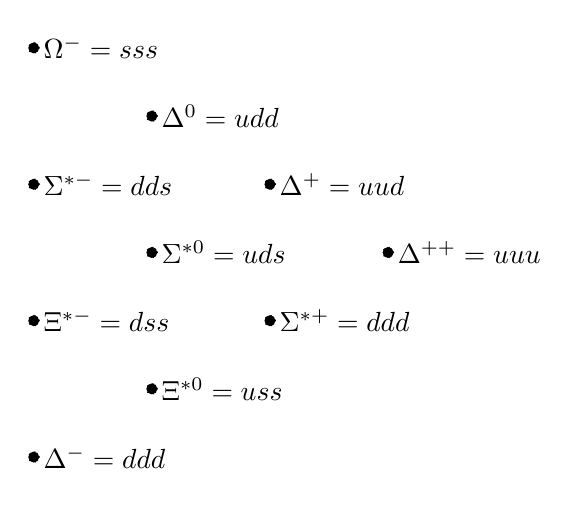
\begin{tikzpicture}[dotted]
  \draw[fill] ({-1.5},{3*sin{60}}) circle [radius=0.07];
  \draw[fill] (0,{2*sin{60}}) circle [radius=0.07];
  \draw[fill] (1.5,{-sin{60}}) circle [radius=0.07];
  \draw[fill] (-1.5,{-3*sin{60}}) circle [radius=0.07];
  \draw[fill] (0,{-2*sin{60}}) circle [radius=0.07];
  \draw[fill] (1.5,{sin{60}}) circle [radius=0.07];
  \draw[fill] (3,0) circle [radius=0.07];
  \draw[fill] (-1.5,{sin{60}}) circle [radius=0.07];
  \draw[fill] (-1.5,{-sin{60}}) circle [radius=0.07];
  \draw[fill] (0,0) circle [radius=0.07];
  \node [right] at (3,0) {$\Delta^{++}=uuu$};
  \node [right] at (0,0) {$\Sigma^{*0}=uds$};
  \node [right] at (-1.5,{-3*sin{60}}) {$\Delta^{-}=ddd$};
  \node [right] at (-1.5,{3*sin{60}}) {$\Omega^{-}=sss$};
  \node [right] at (0,{2*sin{60}}) {$\Delta^{0}=udd$};
  \node [right] at (1.5,{sin{60}}) {$\Delta^{+}=uud$};
  \node [right] at (0,{-2*sin{60}}) {$\Xi^{*0}=uss$};
  \node [right] at (-1.5,{sin{60}}) {$\Sigma^{*-}=dds$};
  \node [right] at (-1.5,{-sin{60}}) {$\Xi^{*-}=dss$};
  \node [right] at (1.5,{-sin{60}}) {$\Sigma^{*+}=ddd$};
\end{tikzpicture}\end{center}}

\newcommand{\baryonoctet}{\begin{center}
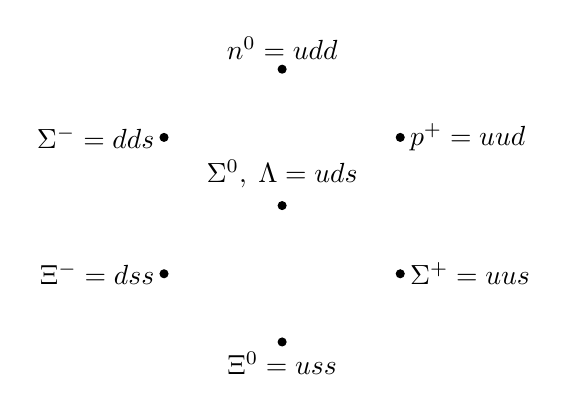
\begin{tikzpicture}
  \draw[fill] (30:{2*sin{60}}) circle [radius=0.05];
  \draw[fill] (90:{2*sin{60}}) circle [radius=0.05];
  \draw[fill] (150:{2*sin{60}}) circle [radius=0.05];
  \draw[fill] (210:{2*sin{60}}) circle [radius=0.05];
  \draw[fill] (270:{2*sin{60}}) circle [radius=0.05];
  \draw[fill] (330:{2*sin{60}}) circle [radius=0.05];
  \draw[fill] (0,0) circle [radius=0.05];
  \node [above] at (0,0.1) {$\Sigma^0,\ \Lambda=uds$};
  \node (0) at (0,0) {};
  \node [right] at (30:{2*sin{60}}) {$p^+=uud$};
  \node (1) at (30:{2*sin{60}}) {};
  \node [above] at (90:{2*sin{60}}) {$n^0=udd$};
  \node (2) at (90:{2*sin{60}}) {};
  \node [left] at (150:{2*sin{60}}) {$\Sigma^-=dds$};
  \node (3) at (150:{2*sin{60}}) {};
  \node [left] at (210:{2*sin{60}}) {$\Xi^-=dss$};
  \node (4) at (210:{2*sin{60}}) {};
  \node [below] at (270:{2*sin{60}}) {$\Xi^0=uss$};
  \node (5) at (270:{2*sin{60}}) {};
  \node [right] at (330:{2*sin{60}}) {$\Sigma^+=uus$};
  \node (6) at (330:{2*sin{60}}) {};
\end{tikzpicture}\end{center}}

% Some more pictures for SU(3)

\newcommand{\slhex}{\begin{center}
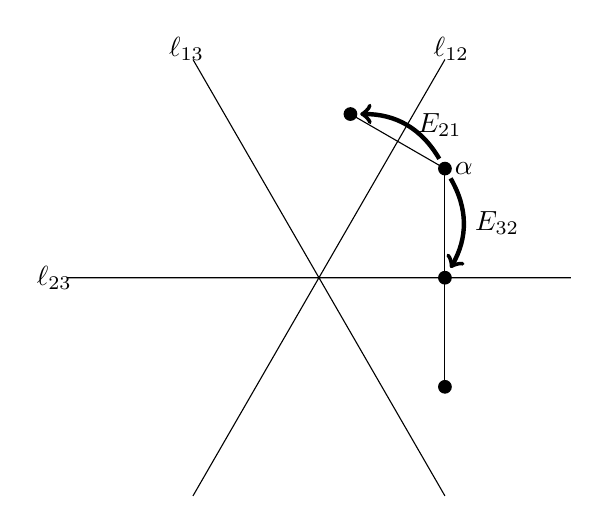
\begin{tikzpicture}[scale=0.8]
  \draw
     (-4,0) -- (4,0)
     (240:4) -- (60:4)
     (120:4) -- (-60:4);
  \node at (-4.2,0) {$\ell_{23}$};
  \node at (60:4.2) {$\ell_{12}$};
  \node at (120:4.2) {$\ell_{13}$};
  \node at (2.3,1.73205080757) {$\alpha$};
  \node (1) at (2,1.73205080757) {};
  \node (2) at (0.5,2.59807621135) {};
  \node (3) at (2,0) {};
  \draw [fill] (2,1.73205080757) circle [radius=0.1];
  \draw [fill] (2,-1.73205080757) circle [radius=0.1];
  \draw [fill] (2,0) circle [radius=0.1];
  \draw [fill] (0.5,2.59807621135) circle [radius=0.1];
  \draw (2,1.73205080757) -- (2,-1.73205080757);
  \draw (2,1.73205080757) -- (0.5,2.59807621135);
  \path[ultra thick,solid,->] 
  (1) edge [bend right] node [right] {$E_{21}$} (2)
  (1) edge [bend left] node [right] {$E_{32}$} (3);
\end{tikzpicture}
\end{center}}

\newcommand{\gtwoadj}{\begin{center}
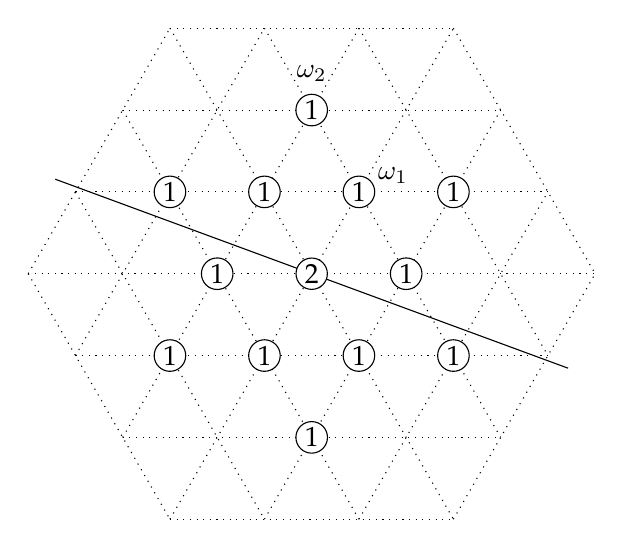
\begin{tikzpicture}[scale=1.2,dotted,bigger node/.style={fill=white,solid,circle,draw,text=black,inner sep=1pt,font=\boldmath}]
  \draw (-3,0) -- (3,0);
  \draw (240:3) -- (60:3);
  \draw (120:3) -- (300:3);
  \draw (-3,0) -- (120:3);
  \draw (-3,0) -- (240:3);
  \draw (120:3) -- (60:3);
  \draw (240:3) -- (300:3);
  \draw (300:3) -- (3,0);
  \draw (60:3) -- (3,0);
  \draw (-2,{2*sin{60}}) -- (2,{2*sin{60}});
  \draw ({-2-cos{60}},{sin{60}}) -- ({2+cos{60}},{sin{60}});
  \draw (-2,{-2*sin{60}}) -- (2,{-2*sin{60}});
  \draw ({-2-cos{60}},{-sin{60}}) -- ({2+cos{60}},{-sin{60}});
  \draw (-2,{2*sin{60}}) -- (2,{2*sin{60}});
  \draw ({-2-cos{60}},{sin{60}}) -- ({-cos{60}},{-3*sin{60}});
  \draw ({-2},{2*sin{60}}) -- ({cos{60}},{-3*sin{60}});
  \draw ({-cos{60}},{3*sin{60}}) -- ({2},{-2*sin{60}});
  \draw ({cos{60}},{3*sin{60}}) -- ({2+cos{60}},{-sin{60}});
  \draw ({cos{60}},{-3*sin{60}}) -- ({2+cos{60}},{sin{60}});
  \draw ({-cos{60}},{-3*sin{60}}) -- ({2},{2*sin{60}});
  \draw ({-2},{-2*sin{60}}) -- ({cos{60}},{3*sin{60}});
  \draw ({-2-cos{60}},{-sin{60}}) -- ({-cos{60}},{3*sin{60}});
  \draw [solid] (-2.7135,1) -- (2.7135,-1);

  \node[bigger node] at (0,0) {2};
  \node[bigger node] at (30:1.73205080757) {1};
  \node[bigger node] at (90:1.73205080757) {1};
  \node[bigger node] at (150:1.73205080757) {1};
  \node[bigger node] at (210:1.73205080757) {1};
  \node[bigger node] at (270:1.73205080757) {1};
  \node[bigger node] at (330:1.73205080757) {1};
  \node[above] at (90:1.93205080757) {$\omega_2$};
  \node[bigger node] at (0:1) {1};
  \node[bigger node] at (60:1) {1};
  \node[bigger node] at (120:1) {1};
  \node[bigger node] at (180:1) {1};
  \node[bigger node] at (240:1) {1};
  \node[bigger node] at (300:1) {1};
  \node[right] at (60:1.2) {$\omega_1$};
\end{tikzpicture}\end{center}}

\newcommand{\gtwoadjpos}{\begin{center}
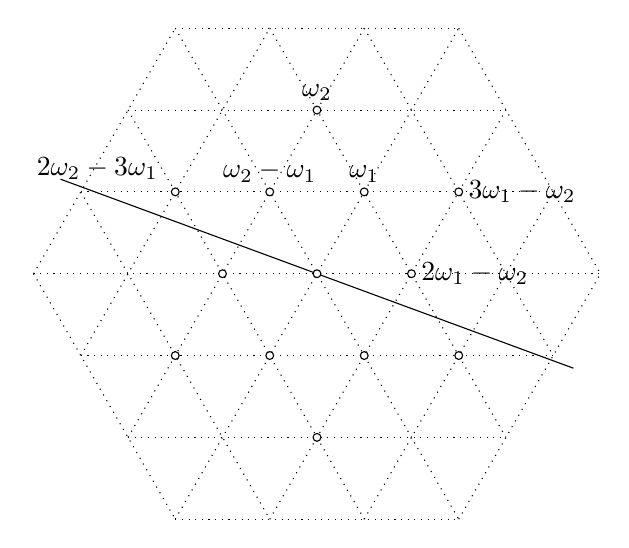
\begin{tikzpicture}[scale=1.2,dotted,bigger node/.style={fill=white,solid,circle,draw,text=black,inner sep=1pt,font=\boldmath}]
  \draw (-3,0) -- (3,0);
  \draw (240:3) -- (60:3);
  \draw (120:3) -- (300:3);
  \draw (-3,0) -- (120:3);
  \draw (-3,0) -- (240:3);
  \draw (120:3) -- (60:3);
  \draw (240:3) -- (300:3);
  \draw (300:3) -- (3,0);
  \draw (60:3) -- (3,0);
  \draw (-2,{2*sin{60}}) -- (2,{2*sin{60}});
  \draw ({-2-cos{60}},{sin{60}}) -- ({2+cos{60}},{sin{60}});
  \draw (-2,{-2*sin{60}}) -- (2,{-2*sin{60}});
  \draw ({-2-cos{60}},{-sin{60}}) -- ({2+cos{60}},{-sin{60}});
  \draw (-2,{2*sin{60}}) -- (2,{2*sin{60}});
  \draw ({-2-cos{60}},{sin{60}}) -- ({-cos{60}},{-3*sin{60}});
  \draw ({-2},{2*sin{60}}) -- ({cos{60}},{-3*sin{60}});
  \draw ({-cos{60}},{3*sin{60}}) -- ({2},{-2*sin{60}});
  \draw ({cos{60}},{3*sin{60}}) -- ({2+cos{60}},{-sin{60}});
  \draw ({cos{60}},{-3*sin{60}}) -- ({2+cos{60}},{sin{60}});
  \draw ({-cos{60}},{-3*sin{60}}) -- ({2},{2*sin{60}});
  \draw ({-2},{-2*sin{60}}) -- ({cos{60}},{3*sin{60}});
  \draw ({-2-cos{60}},{-sin{60}}) -- ({-cos{60}},{3*sin{60}});
  \draw [solid] (-2.7135,1) -- (2.7135,-1);

  \node[bigger node] at (0,0) {};
  \node[bigger node] at (30:1.73205080757) {};
  \node[bigger node] at (90:1.73205080757) {};
  \node[bigger node] at (150:1.73205080757) {};
  \node[bigger node] at (210:1.73205080757) {};
  \node[bigger node] at (270:1.73205080757) {};
  \node[bigger node] at (330:1.73205080757) {};
  \node[bigger node] at (0:1) {};
  \node[bigger node] at (60:1) {};
  \node[bigger node] at (120:1) {};
  \node[bigger node] at (180:1) {};
  \node[bigger node] at (240:1) {};
  \node[bigger node] at (300:1) {};

  \node[right] at (30:1.73205080757) {$3\omega_1-\omega_2$};
  \node[above] at (90:1.73205080757) {$\omega_2$};
  \node[left] at (145:1.93205080757) {$2\omega_2-3\omega_1$};
  \node[right] at (0:1) {$2\omega_1-\omega_2$};
  \node[above] at (60:1) {$\omega_1$};
  \node[above] at (120:1) {$\omega_2-\omega_1$};
\end{tikzpicture}\end{center}}

\newcommand{\gtwolambdaonezero}{\begin{center}
\begin{tikzpicture}[scale=1.2,dotted,bigger node/.style={fill=white,solid,circle,draw,text=black,inner sep=1pt,font=\boldmath}]
  \draw (-3,0) -- (3,0);
  \draw (240:3) -- (60:3);
  \draw (120:3) -- (300:3);
  \draw (-3,0) -- (120:3);
  \draw (-3,0) -- (240:3);
  \draw (120:3) -- (60:3);
  \draw (240:3) -- (300:3);
  \draw (300:3) -- (3,0);
  \draw (60:3) -- (3,0);
  \draw (-2,{2*sin{60}}) -- (2,{2*sin{60}});
  \draw ({-2-cos{60}},{sin{60}}) -- ({2+cos{60}},{sin{60}});
  \draw (-2,{-2*sin{60}}) -- (2,{-2*sin{60}});
  \draw ({-2-cos{60}},{-sin{60}}) -- ({2+cos{60}},{-sin{60}});
  \draw (-2,{2*sin{60}}) -- (2,{2*sin{60}});
  \draw ({-2-cos{60}},{sin{60}}) -- ({-cos{60}},{-3*sin{60}});
  \draw ({-2},{2*sin{60}}) -- ({cos{60}},{-3*sin{60}});
  \draw ({-cos{60}},{3*sin{60}}) -- ({2},{-2*sin{60}});
  \draw ({cos{60}},{3*sin{60}}) -- ({2+cos{60}},{-sin{60}});
  \draw ({cos{60}},{-3*sin{60}}) -- ({2+cos{60}},{sin{60}});
  \draw ({-cos{60}},{-3*sin{60}}) -- ({2},{2*sin{60}});
  \draw ({-2},{-2*sin{60}}) -- ({cos{60}},{3*sin{60}});
  \draw ({-2-cos{60}},{-sin{60}}) -- ({-cos{60}},{3*sin{60}});

  \node[bigger node] at (0,0) {};
  \node[bigger node] at (0:1) {};
  \node[bigger node] at (60:1) {};
  \node[bigger node] at (120:1) {};
  \node[bigger node] at (180:1) {};
  \node[bigger node] at (240:1) {};
  \node[bigger node] at (300:1) {};
  \node[right] at (60:1.2) {$\omega_1$};
\end{tikzpicture}\end{center}}

\newcommand{\gtwolambdatwozero}{\begin{center}
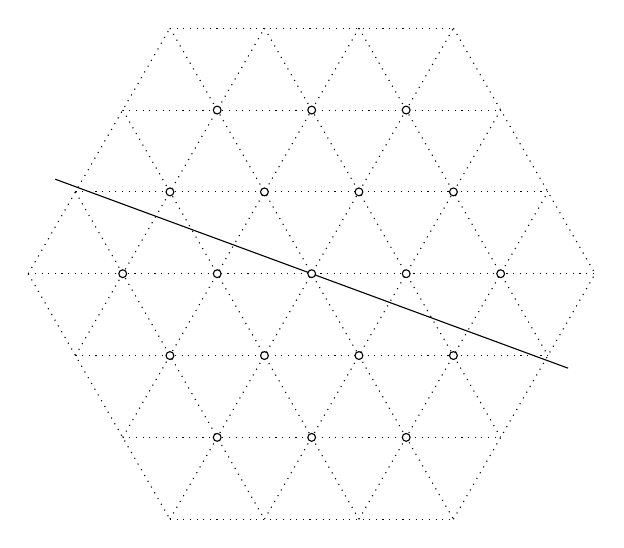
\begin{tikzpicture}[scale=1.2,dotted,bigger node/.style={fill=white,solid,circle,draw,text=black,inner sep=1pt,font=\boldmath}]
  \draw (-3,0) -- (3,0);
  \draw (240:3) -- (60:3);
  \draw (120:3) -- (300:3);
  \draw (-3,0) -- (120:3);
  \draw (-3,0) -- (240:3);
  \draw (120:3) -- (60:3);
  \draw (240:3) -- (300:3);
  \draw (300:3) -- (3,0);
  \draw (60:3) -- (3,0);
  \draw (-2,{2*sin{60}}) -- (2,{2*sin{60}});
  \draw ({-2-cos{60}},{sin{60}}) -- ({2+cos{60}},{sin{60}});
  \draw (-2,{-2*sin{60}}) -- (2,{-2*sin{60}});
  \draw ({-2-cos{60}},{-sin{60}}) -- ({2+cos{60}},{-sin{60}});
  \draw (-2,{2*sin{60}}) -- (2,{2*sin{60}});
  \draw ({-2-cos{60}},{sin{60}}) -- ({-cos{60}},{-3*sin{60}});
  \draw ({-2},{2*sin{60}}) -- ({cos{60}},{-3*sin{60}});
  \draw ({-cos{60}},{3*sin{60}}) -- ({2},{-2*sin{60}});
  \draw ({cos{60}},{3*sin{60}}) -- ({2+cos{60}},{-sin{60}});
  \draw ({cos{60}},{-3*sin{60}}) -- ({2+cos{60}},{sin{60}});
  \draw ({-cos{60}},{-3*sin{60}}) -- ({2},{2*sin{60}});
  \draw ({-2},{-2*sin{60}}) -- ({cos{60}},{3*sin{60}});
  \draw ({-2-cos{60}},{-sin{60}}) -- ({-cos{60}},{3*sin{60}});
  \draw [solid] (-2.7135,1) -- (2.7135,-1);

  \node[bigger node] at (0,0) {};
  \node[bigger node] at (30:1.73205080757) {};
  \node[bigger node] at (90:1.73205080757) {};
  \node[bigger node] at (150:1.73205080757) {};
  \node[bigger node] at (210:1.73205080757) {};
  \node[bigger node] at (270:1.73205080757) {};
  \node[bigger node] at (330:1.73205080757) {};
  \node[bigger node] at (0:1) {};
  \node[bigger node] at (60:1) {};
  \node[bigger node] at (120:1) {};
  \node[bigger node] at (180:1) {};
  \node[bigger node] at (240:1) {};
  \node[bigger node] at (300:1) {};
  \node[bigger node] at (0:2) {};
  \node[bigger node] at (60:2) {};
  \node[bigger node] at (120:2) {};
  \node[bigger node] at (180:2) {};
  \node[bigger node] at (240:2) {};
  \node[bigger node] at (300:2) {};
\end{tikzpicture}\end{center}}

\newcommand{\gtwolabel}{\begin{center}
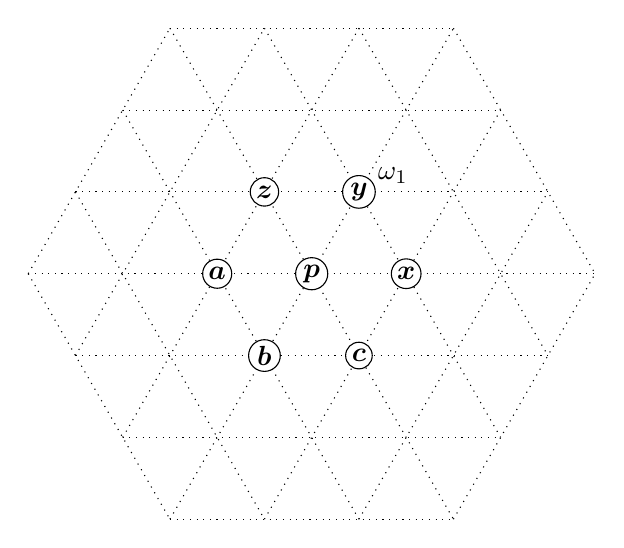
\begin{tikzpicture}[scale=1.2,dotted,bigger node/.style={fill=white,solid,circle,draw,text=black,inner sep=1pt,font=\boldmath}]
  \draw (-3,0) -- (3,0);
  \draw (240:3) -- (60:3);
  \draw (120:3) -- (300:3);
  \draw (-3,0) -- (120:3);
  \draw (-3,0) -- (240:3);
  \draw (120:3) -- (60:3);
  \draw (240:3) -- (300:3);
  \draw (300:3) -- (3,0);
  \draw (60:3) -- (3,0);
  \draw (-2,{2*sin{60}}) -- (2,{2*sin{60}});
  \draw ({-2-cos{60}},{sin{60}}) -- ({2+cos{60}},{sin{60}});
  \draw (-2,{-2*sin{60}}) -- (2,{-2*sin{60}});
  \draw ({-2-cos{60}},{-sin{60}}) -- ({2+cos{60}},{-sin{60}});
  \draw (-2,{2*sin{60}}) -- (2,{2*sin{60}});
  \draw ({-2-cos{60}},{sin{60}}) -- ({-cos{60}},{-3*sin{60}});
  \draw ({-2},{2*sin{60}}) -- ({cos{60}},{-3*sin{60}});
  \draw ({-cos{60}},{3*sin{60}}) -- ({2},{-2*sin{60}});
  \draw ({cos{60}},{3*sin{60}}) -- ({2+cos{60}},{-sin{60}});
  \draw ({cos{60}},{-3*sin{60}}) -- ({2+cos{60}},{sin{60}});
  \draw ({-cos{60}},{-3*sin{60}}) -- ({2},{2*sin{60}});
  \draw ({-2},{-2*sin{60}}) -- ({cos{60}},{3*sin{60}});
  \draw ({-2-cos{60}},{-sin{60}}) -- ({-cos{60}},{3*sin{60}});

  \node[bigger node] at (0,0) {$p$};
  \node[bigger node] at (0:1) {$x$};
  \node[bigger node] at (60:1) {$y$};
  \node[bigger node] at (120:1) {$z$};
  \node[bigger node] at (180:1) {$a$};
  \node[bigger node] at (240:1) {$b$};
  \node[bigger node] at (300:1) {$c$};
  \node[right] at (60:1.2) {$\omega_1$};
\end{tikzpicture}\end{center}}

\newcommand{\gtwolabeltwo}{\begin{center}
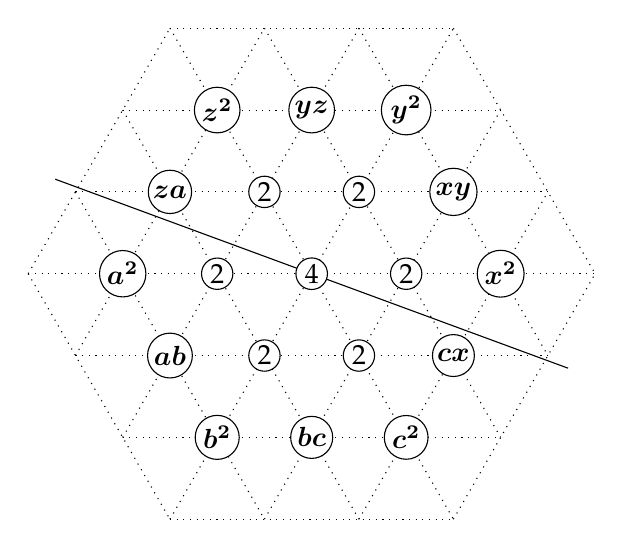
\begin{tikzpicture}[scale=1.2,dotted,bigger node/.style={fill=white,solid,circle,draw,text=black,inner sep=1pt,font=\boldmath}]
  \draw (-3,0) -- (3,0);
  \draw (240:3) -- (60:3);
  \draw (120:3) -- (300:3);
  \draw (-3,0) -- (120:3);
  \draw (-3,0) -- (240:3);
  \draw (120:3) -- (60:3);
  \draw (240:3) -- (300:3);
  \draw (300:3) -- (3,0);
  \draw (60:3) -- (3,0);
  \draw (-2,{2*sin{60}}) -- (2,{2*sin{60}});
  \draw ({-2-cos{60}},{sin{60}}) -- ({2+cos{60}},{sin{60}});
  \draw (-2,{-2*sin{60}}) -- (2,{-2*sin{60}});
  \draw ({-2-cos{60}},{-sin{60}}) -- ({2+cos{60}},{-sin{60}});
  \draw (-2,{2*sin{60}}) -- (2,{2*sin{60}});
  \draw ({-2-cos{60}},{sin{60}}) -- ({-cos{60}},{-3*sin{60}});
  \draw ({-2},{2*sin{60}}) -- ({cos{60}},{-3*sin{60}});
  \draw ({-cos{60}},{3*sin{60}}) -- ({2},{-2*sin{60}});
  \draw ({cos{60}},{3*sin{60}}) -- ({2+cos{60}},{-sin{60}});
  \draw ({cos{60}},{-3*sin{60}}) -- ({2+cos{60}},{sin{60}});
  \draw ({-cos{60}},{-3*sin{60}}) -- ({2},{2*sin{60}});
  \draw ({-2},{-2*sin{60}}) -- ({cos{60}},{3*sin{60}});
  \draw ({-2-cos{60}},{-sin{60}}) -- ({-cos{60}},{3*sin{60}});
  \draw [solid] (-2.7135,1) -- (2.7135,-1);

  \node[bigger node] at (0,0) {4};
  \node[bigger node] at (30:1.73205080757) {$xy$};
  \node[bigger node] at (90:1.73205080757) {$yz$};
  \node[bigger node] at (150:1.73205080757) {$za$};
  \node[bigger node] at (210:1.73205080757) {$ab$};
  \node[bigger node] at (270:1.73205080757) {$bc$};
  \node[bigger node] at (330:1.73205080757) {$cx$};
  \node[bigger node] at (0:1) {2};
  \node[bigger node] at (60:1) {2};
  \node[bigger node] at (120:1) {2};
  \node[bigger node] at (180:1) {2};
  \node[bigger node] at (240:1) {2};
  \node[bigger node] at (300:1) {2};
  \node[bigger node] at (0:2) {$x^2$};
  \node[bigger node] at (60:2) {$y^2$};
  \node[bigger node] at (120:2) {$z^2$};
  \node[bigger node] at (180:2) {$a^2$};
  \node[bigger node] at (240:2) {$b^2$};
  \node[bigger node] at (300:2) {$c^2$};
\end{tikzpicture}\end{center}}

\newcommand{\gtwolambdathree}{\begin{center}
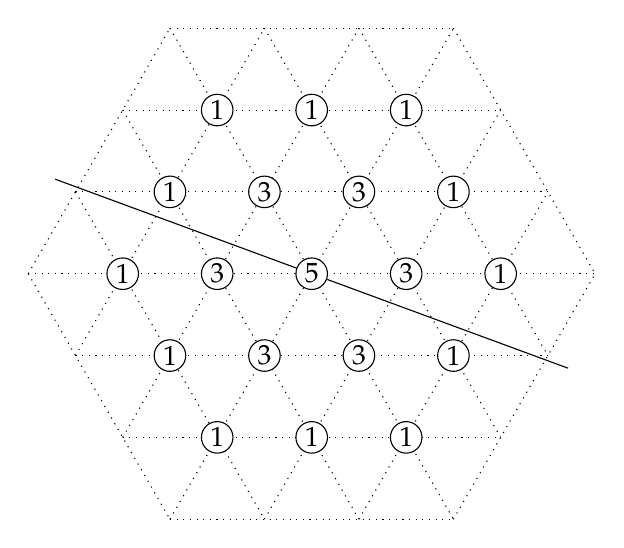
\begin{tikzpicture}[scale=1.2,dotted,bigger node/.style={fill=white,solid,circle,draw,text=black,inner sep=1pt,font=\boldmath}]
  \draw (-3,0) -- (3,0);
  \draw (240:3) -- (60:3);
  \draw (120:3) -- (300:3);
  \draw (-3,0) -- (120:3);
  \draw (-3,0) -- (240:3);
  \draw (120:3) -- (60:3);
  \draw (240:3) -- (300:3);
  \draw (300:3) -- (3,0);
  \draw (60:3) -- (3,0);
  \draw (-2,{2*sin{60}}) -- (2,{2*sin{60}});
  \draw ({-2-cos{60}},{sin{60}}) -- ({2+cos{60}},{sin{60}});
  \draw (-2,{-2*sin{60}}) -- (2,{-2*sin{60}});
  \draw ({-2-cos{60}},{-sin{60}}) -- ({2+cos{60}},{-sin{60}});
  \draw (-2,{2*sin{60}}) -- (2,{2*sin{60}});
  \draw ({-2-cos{60}},{sin{60}}) -- ({-cos{60}},{-3*sin{60}});
  \draw ({-2},{2*sin{60}}) -- ({cos{60}},{-3*sin{60}});
  \draw ({-cos{60}},{3*sin{60}}) -- ({2},{-2*sin{60}});
  \draw ({cos{60}},{3*sin{60}}) -- ({2+cos{60}},{-sin{60}});
  \draw ({cos{60}},{-3*sin{60}}) -- ({2+cos{60}},{sin{60}});
  \draw ({-cos{60}},{-3*sin{60}}) -- ({2},{2*sin{60}});
  \draw ({-2},{-2*sin{60}}) -- ({cos{60}},{3*sin{60}});
  \draw ({-2-cos{60}},{-sin{60}}) -- ({-cos{60}},{3*sin{60}});
  \draw [solid] (-2.7135,1) -- (2.7135,-1);

  \node[bigger node] at (0,0) {5};
  \node[bigger node] at (30:1.73205080757) {1};
  \node[bigger node] at (90:1.73205080757) {1};
  \node[bigger node] at (150:1.73205080757) {1};
  \node[bigger node] at (210:1.73205080757) {1};
  \node[bigger node] at (270:1.73205080757) {1};
  \node[bigger node] at (330:1.73205080757) {1};
  \node[bigger node] at (0:1) {3};
  \node[bigger node] at (60:1) {3};
  \node[bigger node] at (120:1) {3};
  \node[bigger node] at (180:1) {3};
  \node[bigger node] at (240:1) {3};
  \node[bigger node] at (300:1) {3};
  \node[bigger node] at (0:2) {1};
  \node[bigger node] at (60:2) {1};
  \node[bigger node] at (120:2) {1};
  \node[bigger node] at (180:2) {1};
  \node[bigger node] at (240:2) {1};
  \node[bigger node] at (300:2) {1};
\end{tikzpicture}\end{center}}

\newcommand{\gtwodynkin}{\begin{center}
  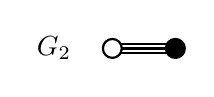
\begin{tikzpicture}[scale=.4]
    \draw (-1,0) node[anchor=east]  {$G_2$};
    \draw[thick] (0 ,0) circle (.3 cm);
    \draw[thick,fill=black] (2 cm,0) circle (.3 cm);
    \draw[thick] (30: 3mm) -- +(1.5 cm, 0);
    \draw[thick] (0: 3 mm) -- +(1.4 cm, 0);
    \draw[thick] (-30: 3 mm) -- +(1.5 cm, 0);
  \end{tikzpicture}
\end{center}}



%%% Local Variables: 
%%% mode: latex
%%% TeX-master: "master"
%%% End: 

\title{Geometry and Groups}
\author{Jonny Evans}

\begin{document}

\maketitle

The notation $1$ may refer to the number one or to the identity matrix or to the identity element in any group. It should be clear what is meant from the context, so please try not to get confused!

\section{Symmetries of polytopes}

\subsection{Isometries}

This is a course about symmetry. For us, a symmetry will be a distance-preserving transformation, otherwise known as an {\em isometry}:

\begin{dfn}
An isometry of $\RR^n$ is a distance-preserving bijection $T\colon\RR^n\to\RR^n$, that is
\[|T(x)-T(y)|=|x-y|\]
for all $x,y\in\RR^n$. We will write $\OP{Isom}(\RR^n)$ for the group of all isometries. If $P\subset\RR^n$ is a subset then we define the symmetry group of $P$ to be the subgroup
\[\OP{Sym}(P)\{T\in\OP{Isom}(\RR^n)\ :\ TP=P\},\]
where $TP=P$ means ``$T(x)\in P$ if and only if $x\in P$''.
\end{dfn}

\begin{exm}
For example, the symmetries of an equilateral triangle $P$ comprise the three reflections in its lines of symmetry and the three rotations about its centre of mass by $0$, $2\pi/3$ and $4\pi/3$ radians. This is isomorphic to the group $S_3$ of permutations of three objects.
\end{exm}

\begin{exm}
If $b\in\RR^n$ then the translation $T(x)=x+b$ is an isometry:
\[|T(x)-T(y)|=|(x+b)-(y+b)|=|x-y|.\]
\end{exm}

\begin{exm}
If $A$ is an $n$-by-$n$ orthogonal matrix (that is $A^TA=1$) then $T(x)=Ax$ is an isometry (an orthogonal transformation):
\begin{align*}
|T(x)-T(y)|^2&=|A(x-y)|^2\\
&=(A(x-y))^T(A(x-y))\\
&=(x-y)^TA^TA(x-y)\\
&=(x-y)^T(x-y)\\
&=|x-y|^2
\end{align*}
where we have used the formula $|v|^2=v^Tv$ for vectors $v\in\RR^n$ and the fact that $(Av)^T=v^TA^T$. We write $O(n)$ for the group of orthogonal matrices. Orthogonal transformations include rotations and reflections through hyperplanes containing 0.

For example, the matrix
\[\left(\begin{array}{cc}
\cos\theta&-\sin\theta\\
\sin\theta&\cos\theta
\end{array}\right)\]
defines a rotation through an angle $\theta$ about the origin; the matrix
\[\left(\begin{array}{cc}
1&0\\
0&-1
\end{array}\right)\]
defines a reflection in the $x$-axis.

Recall that if $A\in O(n)$ then $\det(A)=\pm 1$ (because $\det(A)^2=\det(A^T)\det(A)=\det(A^TA)=\det(1)=1$). If $\det(A)=1$, we say that $A$ is orientation-preserving; if $\det(A)=-1$, we say that $A$ is orientation-reversing. We write $SO(n)$ for the subgroup of orientation-preserving orthogonal matrices.
\end{exm}

We will see later in the course that actually any $T\in\OP{Isom}(\RR^n)$ has the form
\[T(x)=Ax+b\]
for some $A\in O(n)$ and $b\in\RR^n$.

\begin{dfn}
We will write $\OP{Isom}^+(\RR^n)$ for the subgroup of orientation-preserving isometries, that is $T(x)=Ax+b$ for $A\in SO(n)$. If $P\subset\RR^n$ is a subset, we write $\OP{Sym}^+(P)$ for the subgroup of orientation-preserving symmetries of $P$.
\end{dfn}

\begin{exm}
If $P$ is a regular $n$-gon then the group of symmetries comprises $n$ reflections and $n$ rotations (including the identity). It is called the dihedral group\footnote{Some people (including, sometimes, me) call this the dihedral group $D_n$ - be careful of the notation. For us, the subscript is the size of the group.} $D_{2n}$.
\end{exm}

The aim of this first section is to compute the symmetry groups for some more complicated 3- and higher-dimensional polytopes.

\subsection{The regular tetrahedron}

\begin{exm}[The regular tetrahedron]
The regular tetrahedron $\mathbf{T}$ has four vertices and its symmetries permute those vertices, so we get a map $A\colon \OP{Sym}(\mathbf{T})\to S_4$ which sends each symmetry to the corresponding permutation. Explicitly, $A(T)$ is the permutation sending the vertex $v$ to the vertex $Tv$, i.e.
\[A(T)(v)=T(v).\]
I claim that $A$ is (a) a homomorphism, (b) surjective, (c) injective, and hence it is an isomorphism so we will see that $\OP{Sym}(\mathbf{T})\cong S_4$.

\begin{enumerate}
\item[(a)] If $T=1\in\OP{Sym}(\mathbf{T})$ then it doesn't move the vertices at all, so acts as the identity permutation. Therefore $A(1)=1$. Moreover, if $T_1,T_2\in\OP{Sym}(\mathbf{T})$ and if $v$ is a vertex then
\begin{align*}
A(T_1\circ T_2)(v)&=(T_1\circ T_2)(v)\\
&=T_1(T_2(v))\\
&=A(T_1)(A(T_2)(v))\\
&=(A(T_1)\circ A(T_2))(v)
\end{align*}
so $A(T_1)\circ A(T_2)=A(T_1\circ T_2)$. This proves that $A$ is a homomorphism.

\item[(b)] To see that $A$ is surjective, we need to find, for every permutation of the vertices, a symmetry of $\mathbf{T}$ which effects this permutation. We will (i) first find a symmetry when the permutation is a transposition (switching two vertices and fixing the other two). (ii) We then recall from basic group theory that the permutation group is generated by transpositions. (iii) Finally, we will prove that if $A\colon G\to H$ is a homomorphism and the image of $A$ contains a generating set, then $A$ is surjective.

\begin{enumerate}
\item[(i)] Suppose you want to switch the vertices $p$ and $q$, leaving $r$ and $s$ fixed. Pick the unique plane containing $r$ and $s$ which is orthogonal to the edge $pq$. The reflection in this plane is a symmetry which effects the desired transposition.
\item[(ii)] Recall that the permutation group is generated by transpositions; in other words, any permutation can be written as a composition of transpositions. To see this, we work by induction on the number of objects being permuted: if there are only two objects then there are only two permutations (the identity and a transposition) so the claim is certainly true; if there are $n+1$ objects $s_1,\ldots,s_{n+1}$ and $\sigma$ is an arbitrary permutation then let $\tau$ be the permutation that switches $\sigma(s_{n+1})$ and $s_{n+1}$ (unless these happen to be equal, in which case let $\tau=1$); the permutation $\tau\circ\sigma$ fixes $s_{n+1}$, and is therefore a permutation of the first $n$ objects; by induction it can be written as a composition of transpositions, so including $\tau$ as the final transposition we find that we can write $\sigma$ as a composition of transpositions.
\item[(iii)] If $A\colon G\to H$ is a homomorphism and the image of $A$ contains a generating set $h_1,\ldots,h_m$ then we know that there exist elements $g_i$ such that $A(g_i)=h_i$ for all $i$. Since any element $h\in H$ can be written as a product $h_{i_1}^{\pm 1}\cdots h_{i_k}^{\pm 1}$ of generators (or their inverses), we see that
\[h=A(g_{i_1}^{\pm 1})\cdots A(g_{i_k}^{\pm 1})=A(g_{i_1}^{\pm 1}\cdots g_{i_k}^{\pm 1}),\]
so $h$ is in the image of $A$ for all $h\in H$, and $A$ is surjective.
\end{enumerate}
This proves surjectivity of $A$.

\item[(c)] To see injectivity, it is necessary and sufficient to show that the kernel of $A$ is trivial\footnote{If $F\colon G\to H$ is a homomorphism of groups then its kernel is the subgroup $\ker(F):=\{g\in G\ :\ F(g)=1\}$. If the kernel is $\{1\}$ then $F(g)=F(h)$ implies $F(gh^{-1})=1$, so $gh^{-1}=1$ and $g=h$; therefore $\ker(F)=\{1\}$ implies $F$ is injective. Conversely, if $F$ is injective then $F^{-1}(1)$ contains only one element, $1$.}. The kernel of $A$ is the set of symmetries of $\mathbf{T}$ which leave every vertex fixed. In a few lectures' time, we will see that if an isometry $T$ of $\RR^n$ fixes $n+1$ vectors $a_0,\ldots,a_n$ such that $a_1-a_0,\ldots,a_n-a_0$ form a basis of $\RR^n$ then $T$ is the identity. In our case we can apply this where $a_0,\ldots,a_3$ are the vertices of the tetrahedron $\mathbf{T}$ to deduce that if $T\in\ker(A)$ then $T$ is the identity. Hence $A$ is injective.
\end{enumerate}
This proves that the symmetry group of a regular tetrahedron is isomorphic to the group of permutations of four objects.
\end{exm}

What about $\OP{Sym}^+(\mathbf{T})$? On the one hand, $S_4$ is generated by transpositions. On the other hand, these correspond under $A$ to reflections. Note that a reflection is orientation-reversing, and a product of $k$ reflections is orientation-preserving if and only if $k$ is even (because $\det(M_1\cdots M_k)=\det(M_1)\cdots\det(M_k)=(-1)^k$ if each $M_i$ is a reflection). Therefore the {\em alternating group} $A_4$ of even permutations (which can be written as an even number of transpositions) correspond to the orientation-preserving symmetries of $\mathbf{T}$, that is
\[\OP{Sym}^+(\mathbf{T})\cong A_4.\]

\subsection{Group actions}

If we try and generalise the example of the regular tetrahedron naively, we run into problems. For example, a cube has eight vertices, but not all of the permutations of these vertices can be realised by symmetries of the cube. Nonetheless, we can abstract many of the important ideas from the example of the tetrahedron into a powerful tool we call the theory of {\em group actions}. This gives us a systematic way of studying questions about symmetry.

\begin{dfn}
  Let $G$ be a group and $X$ be a set. Let $\OP{Perm}(X)$ be the group of permutations of $X$. An action of $G$ on $X$ is a homomorphism
  \[A\colon G\to\OP{Perm}(X).\]
  Almost always, we will write $A(g)(x)$ as $gx$.
\end{dfn}

\begin{exm}
  Let $P\subset\RR^n$ and consider $G:=\OP{Sym}(P)\subset\OP{Isom}(\RR^n)$ be the symmetry group of $P$. Then there is a $G$-action on $P$: any $g\in G$ gives us the permutation $x\mapsto gx$. If $P$ is a polyhedron in $\RR^3$, for example, this restricts to an action of $G$ on the set of vertices of $P$, on the set of edges of $P$, on the set of faces of $P$,...
\end{exm}

\begin{thm}[Orbit-Stabiliser Theorem]
  If $G$ acts on a set $X$ then, for each $x\in X$, define
  \begin{itemize}
  \item $\OP{Orb}(x):=\{y\in X\ :\ y=gx\mbox{ for some }g\in G\}$, the orbit of $x$;
  \item $\OP{Stab}(x):=\{g\in\ G\ :\ gx=x\}$, the stabiliser of $x$.
  \end{itemize}
  Then, for each $x\in X$, there is a bijection between the cosets $G/\OP{Stab}(x)$ and the orbit $\OP{Orb}(x)$. In particular, if $G$ and $X$ are finite then $|\OP{Orb}(x)|\cdot|\OP{Stab}(x)|=|G|$.  
\end{thm}
\begin{proof}
The bijection $G/\OP{Stab}(x)\to\OP{Orb}(x)$ is $[g]\mapsto gx$. This is well-defined because if $[g_1]=[g_2]$ then $g_2=g_1h$ for some $h\in\OP{Stab}(x)$, hence $g_2x=g_1hx=g_1x$. It is injective because if $g_1x=g_2x$ then $g_2^{-1}g_1x=x$ so $g_2^{-1}g_1\in\OP{Stab}(x)$ and $g_1\OP{Stab}(x)=g_2\OP{Stab}(x)$. It is surjective because if $y\in\OP{Orb}(x)$ then there exists $g_0\in G$ such that $y=g_0x$, hence $[g_0]\mapsto y$.
\end{proof}

\begin{exm}
Consider the equilateral triangle $P$ and look at the action of $\OP{Sym}(P)$ on its vertices. There are three vertices and any one can be mapped to any other by a symmetry, so there is only one orbit of size 3. The stabiliser of a vertex comprises the identity and the reflection about the line of symmetry passing through that vertex; in other words, it has size 2. Therefore by the orbit-stabiliser theorem, the size of $\OP{Sym}(P)$ is 6 (3 times 2).
\end{exm}

This example has the special property that there is only one orbit. In this case we say that the action is {\em transitive}. Here is an example where the action is not transitive:

\begin{exm}
Let $P$ be the pentagonal bipyramid, in other words, the polyhedron which intersects the $xy$-plane in a regular pentagon of sidelength 1 and has two vertices at $(0,0,\pm h)$ so that the sides connecting the vertices of the pentagon to $(0,0,\pm h)$ also have length 1. The group of symmetries of $P$ acts on the set of vertices. There are two orbits: the vertices $p_1,\ldots,p_5$ form an orbit and the vertices $(0,0,\pm h)$ form an orbit. The stabiliser of $(0,0,h)$ is the symmetry group of the pentagon, so the total number of symmetries is two (the number of vertices in the orbit of $(0,0,h)$) times ten (the number of symmetries fixing $(0,0,h)$), that is 20. Alternatively, if we look at the stabiliser of $p_1$ we see there are four elements: the identity, the reflection in the vertical plane through $p_1$ and 0, the reflection in the $xy$-plane, and the 180 degree rotation around the $p_1$-axis. The size of the orbit of $p_1$ is five, so the total number of symmetries is (again) 20.
\end{exm}

\begin{exm}
  Let's look again at the tetrahedron. The action of symmetries on faces gives a homomorphism $\OP{Sym}(T)\to S_4$. As I explained earlier, an isometry is determined by its action on four vectors $a_1,a_2,a_3,a_4$ such that $a_2-a_1,a_3-a_1,a_4-a_1$ forms a basis, and we can take these vectors to be the midpoints of the faces, so that the isometry is determined by its action on faces. Therefore this is an injective homomorphism.

  The orbit-stabiliser theorem tells us that $|\OP{Sym}(T)|$ is equal to the size of the orbit times the size of the stabiliser. The orbit of a face is the set of of all face (we say the action is {\em transitive}) and there are four. The stabiliser of a single face is the dihedral group $D_6$: any symmetry of the triangular face is the restriction of a symmetry of the tetrahedron. The orbit stabiliser theorem now implies $|\OP{Sym}(T)|=4\times 6=24$. Therefore the homomorphism $\OP{Sym}(T)\to S_4$ must be bijective (it's an injective map between sets of the same size) hence an isomorphism.
\end{exm}

\begin{exm}
Alternatively, one could look at the action on vertices. The only difficulty is in working out the stabiliser of a vertex. For this, we look at the vertex figure at $x$: take the faces incident at $x$ and project them onto the plane orthogonal to the line through $0$ and $x$. This gives an equilateral triangle in the case of $T$. A symmetry of $T$ stabilising a vertex (a ``vertex-stabiliser'') induces a symmetry of the corresponding vertex figure. It is easy to see that, in this case, every symmetry of the vertex figure is realised by a vertex-stabiliser. Therefore the vertex stabiliser group is isomorphic to the symmetry group of the vertex figure, namely $D_6$.
\end{exm}

\begin{exm}
Similarly, this tells us that the number of symmetries of a cube $C$ must be 48: there is an action of $\OP{Sym}(C)$ on the eight vertices. Any vertex can be mapped to any other, and I claim that $\OP{Stab}(x)\cong D_6$. To see this, observe that the vertex figure of a cube is an equilateral triangle. Any symmetry of $C$ fixing a vertex $x$ acts on the vertex figure of the cube and hence defines an element of $D_6$. As before, an isometry fixing a vertex is determined by the action on the vertex figure, and any symmetry of the vertex figure can be realised (in this case). Therefore $|G|=8\times 6=48$.
\end{exm}

\begin{exm}
  Let us just consider the rotational symmetries of the cube. Only the rotational symmetries of the vertex figure can be realised, so the vertex stabiliser is $C_3$ and there are only 24 symmetries in total. In fact, we can see that $\OP{Sym}^+(P)\cong S_4$. Consider the set $X$ comprising the four axes through of opposite vertices. There is a $G$-action on this set which permutes these four axes, which gives a homomorphism $G\to S_4$. This is surjective: again it suffices to find rotations which effect any given transposition. This can be achieved with rotations about the axis through the midpoints of opposite edges [picture]. Therefore it is an isomorphism.

  Had we done this with the full symmetry group (including reflections) then the symmetry $x\mapsto -x$ would have fixed each of the four axes, so this homomorphism would have failed to be injective. In fact, $\OP{Sym}(C)=S_4\times C_2$, as we will see on a problem sheet.
\end{exm}

\begin{rmk}
What is the relationship between $T$ and $C$? Why does the permutation group $S_4$ show up in both cases? You can inscribe a tetrahedron in a cube using four of the eight vertices. There are precisely two ways to do this. The symmetry group $\OP{Sym}^+(C)\cong S_4$ acts on these two inscribed tetrahedra, giving a homomorphism $S_4\to S_2$. The stabiliser of a single tetrahedron is $\OP{Sym}^+(T)\cong A_4$. The stabiliser of a tetrahedron is the subgroup of $\OP{Sym}^+(C)$ which act as the identity, i.e. it is the kernel of the homomorphism $S_4\to S_2$. Therefore we get the usual identity $S_4/A_4\cong S_2$ (I like to write this as an exact sequence $1\to A_4\to S_4\to S_2\to 1$, where exactness means that the kernel of each map equals the image of the preceding map).
\end{rmk}

\begin{dfn}
Let $P$ be a polyhedron. Put a vertex at the centre of every face and you get a new polyhedron, the dual. Taking dual twice gives the original polyhedron. For example, the dual of $T$ is $T$. The dual of $C$ is an octahedron $O$ (and, dually, the dual of $O$ is $C$). The dual of a dodecahedron $D$ is an icosahedron $I$ (and vice versa). Any symmetry of a polyhedron induces a symmetry of its dual and vice versa, so a polyhedron and its dual have the same symmetry groups. In particular, $\OP{Sym}^+(O)\cong S_4$.
\end{dfn}

\begin{exm}
  The dodecahedron $D$ has 12 pentagonal faces. Therefore the orbit-stabiliser theorem tells us that $|\OP{Sym}(D)|=12\times 5=120$, $|\OP{Sym}^+(D)|=60$; this is because the stabiliser of a face is the symmetry group $D_{10}$ of a pentagon. In fact, $\OP{Sym}^+(D)\cong A_5$. We can see this by inscribing five cubes in $D$. These cubes are permuted by $\OP{Sym}^+(D)$, giving a homomorphism $\OP{Sym}(D)\to S_5$. We can check that this is surjective onto $A_5$ by finding rotational symmetries of $D$ which effect permutations which generate $A_5$. Similarly, $\OP{Sym}^+(I)\cong A_5$.

  How to check that these inscribed objects are really cubes? [picture] It is easy to see that the graph $G$ you get by connecting vertices by diagonals this way is homeomorphic to a cube. Clearly, since all the diagonals have the same length, the edges of $G$ all have the same length. We will now show that any two of them meet at a right angle, and that will suffice to show that $G$ is a cube. Consider the edges $uv$ and $vw$. Let $x$ and $y$ be as in the picture. Then $x$ and $y$ are equidistant from both $w$ and $v$, therefore the line $xy$ is orthogonal to $wv$. The line $uv$ is parallel to $xy$, and hence orthogonal to $wv$.
\end{exm}

\begin{rmk}
  As with the cube, it is an exercise to show that $\OP{Sym}(D)=A_5\times C_2$.
\end{rmk}

\begin{exm}
The 4-dimensional version of the tetrahedron has five tetrahedral faces. By the orbit-stabiliser theorem, this has $5\times 24=120$ symmetries.
\end{exm}

\subsection{Convex polytopes}

Recall that if $x$ and $y$ are vectors in $\RR^n$ then $tx+(1-t)y$, $0\leq t\leq 1$, is a parametrisation of the straight line segment through $x$ and $y$.

\begin{dfn}
  The {\em convex hull} of a finite set of points $X\subset\RR^n$ is the set
  \[\OP{Conv}(X)\left\{\sum_{x\in X}t_xx\ :\ t_x\geq 0\mbox{ for each }x\in X,\ \sum_{x\in X}t_x=1\right\}\]
    A {\em convex polytope} in $\RR^n$ is a compact subset of $\RR^n$ which is the convex hull of a finite set of points.
\end{dfn}

\begin{rmk}
  A set $P\subset\RR^n$ is convex if the straight line segment between two points of $P$ is itself contained in $P$. Exercise: The convex hull of a finite set of points is convex!
\end{rmk}

\begin{dfn}
  Suppose $P=\OP{Conv}(X)$ is a convex polytope. A point $x\in X$ is called a vertex of $P$ if $x\not\in\OP{Conv}(X\setminus\{x\})$. Exercise: A convex polytope is the convex hull of its vertices, i.e. you can drop something that isn't a vertex without changing the convex hull. From now on we will just assume when we write $P=\OP{Conv}(X)$ that $X$ is the set of vertices of $P$. The interior of $P$ is the set
  \[\OP{Int}(P):=\left\{\sum_{x\in X}t_xx\ :\ t_x>0\mbox{ for each }x\in X,\ \sum_{x\in X}t_x=1\right\}\]
  and the boundary of $P$ is the set $\partial P:=P\setminus\OP{Int}(P)$. We will assume WLOG that $\OP{Int}(P)$ is an open set in $\RR^n$, which means that $P$ is an $n$-dimensional polytope. The boundary of a convex polytope is stratified by lower-dimensional {\em faces}:
  \begin{itemize}
  \item zero-dimensional 0-faces (vertices!),
  \item one-dimensional 1-faces (edges!) connecting pairs of vertices,
  \item two-dimensional 2-faces (faces!) spanning collections of edges,
  \item ...
  \item $(n-3)$-faces (``peaks''), i.e. {\em co}dimension 3,
  \item $(n-2)$-faces (``ridges''), codimension 2,
  \item $(n-1)$-faces (``facets''), codimension 1.
  \end{itemize}
  These faces are themselves convex polytopes (obtained by setting some of the coefficients $t_x$ equal to zero).
\end{dfn}

\begin{exm}
The tetrahedron has four vertices, six edges and four faces.
\end{exm}

\begin{dfn}
  A {\em flag} in an $n$-dimensional polytope $P$ is a sequence $\mathbf{f}=(f_0\subset f_1\subset\cdots\subset f_{n-1})$ where $f_k$ is a $k$-face of $P$. A convex polytope is called {\em regular} if, for any two flags $\mathbf{f}$, $\mathbf{f}'$ there exists an isometry $T$ of $\RR^n$ such that $Tf_k=f'_k$.
\end{dfn}

A flag is called a flag for the following reason. Consider a tetrahedron. A flag in a tetrahedron consists of a vertex $v$, an edge $e$ containing $v$ and a triangle $t$ containing $e$. If you stand the edge up vertically with $v$ at the top then the whole thing looks like a flag ($t$) with a flagpole ($e$) and a little knob on top ($v$) keeping the flag in place.

Regular convex polytopes are classified by their {\em Schl\"afli symbol}, which is defined recursively as follows:

\begin{dfn}
The Schl\"afli symbol of a regular convex $p$-gon $\{p\}$. The Schl\"afli symbol of a regular convex polyhedron with $q$ copies of $\{p\}$ meeting at each vertex is $\{p,q\}$. The Schl\"afli symbol of a regular convex 4-polytope with $r$ copies of $\{p,q\}$ meeting along each edge is $\{p,q,r\}$. The Schl\"afli symbol of a regular convex $n$-polytope with $p_{n-1}$ copies of $\{p_1,\ldots,p_{n-2}\}$ meeting along each ridge is $\{p_1,\ldots,p_{n-1}\}$. [Note: All $p_i>2$.] Note that if $P$ has Schl\"afli symbol $\{p_1,\ldots,p_n\}$ then its dual has Sch\"afli symbol $\{p_n,\ldots,p_1\}$.
\end{dfn}

\begin{thm}
  If two regular convex polytopes have the same Schl\"afli symbol then they are congruent by an isometry of $\RR^n$. The vertex figure of a regular convex polytope with Schl\"afli symbol $\{p_1,\ldots,p_n\}$ is a regular convex polytope with Schl\"afli symbol $\{p_2,\ldots,p_n\}$. Any vertex-stabiliser induces a symmetry of the vertex figure at that vertex. If the convex polytope is regular then for any symmetry of the vertex figure there exists a unique vertex-stabiliser which induces it.
\end{thm}

\begin{exm}
  The Schl\"afli symbol of a tetrahedron is $\{3,3\}$.
\end{exm}

\begin{thm}
  There are precisely five 3-dimensional regular convex polytopes, with Schl\"afli symbols:
  \[\{3,3\},\ \{3,4\},\ \{3,5\},\ \{4,3\},\ \{5,3\}.\]
  These are the tetrahedron, octahedron, icosahedron, cube and dodecahedron respectively (the Platonic solids).
\end{thm}
\begin{proof}
  (Sketch.) Note that the internal angle at a vertex of $\{p\}$ is $\pi\left(1-\frac{2}{p}\right)$ and so if there are $q$ meeting at every vertex (i.e. Schl\"afli symbol $\{p,q\}$) then, in order for the polytope to be convex at each vertex, we must have
  \[q\pi\left(1-\frac{2}{p}\right)<2\pi\]
  or
  \[\frac{1}{2}<\frac{1}{p}+\frac{1}{q}.\]
  The only possibilities are the ones listed.
\end{proof}

\subsection{Four dimensions}

There are six possibilities in dimension 4! These are:

\begin{tabular}{c|lr}
  $\{3,3,3\}$ & 5-cell/4-simplex & five tetrahedral facets\\
  $\{3,3,4\}$ & 16-cell/4-orthoplex & 16 tetrahedral facets\\
  $\{3,3,5\}$ & 600-cell & 600 tetrahedral facets\\
  $\{3,4,3\}$ & 24-cell & 24 octahedral facets\\
  $\{4,3,3\}$ & 8-cell/4-cube/tesseract & eight cubical facets\\
  $\{5,3,3\}$ & 120-cell & 120 dodecahedral facets
\end{tabular}

This is proved by a similar argument as in the 3-dimensional case:
\begin{itemize}
\item $\{p,q\}$ and $\{q,r\}$ must be the Schl\"afli symbols of Platonic solids.
\item Moreover, the dihedral angles around each ridge must add up to $2\pi$.
\end{itemize}
Exercise: Look up or calculate the dihedral angles for each Platonic solid and hence (or otherwise) prove the classification of 4-dimensional regular convex polytopes.

In higher dimensions, there are always three regular convex polytopes! These are
\begin{itemize}
\item $\{3,3,3,\ldots,3\}$ ($n$-simplex),
\item $\{4,3,3,\ldots,3\}$, ($n$-cube),
\item $\{3,3,\ldots,3,4\}$ ($n$-orthoplex).
\end{itemize}

\newpage


\section{Isometries of Euclidean space}

\subsection{Pythagoras's theorem}

\begin{thm}
If $\Delta$ is a right-angled triangle with side-lengths $a,b,c$ ($c$ being opposite the right-angle) then $c^2=a^2+b^2$.
\end{thm}
\begin{proof}
Drop a perpendicular from the vertex with the right-angle to the side $c$. This divides the triangle into two smaller triangles $\Delta_1$ and $\Delta_2$. If $A(\Delta)$ denotes the area of $\Delta$ then $A(\Delta)=A(\Delta_1)+A(\Delta_2)$. The three triangles are similar: they all have the same angles. The hypotenuse of $\Delta_1$ is $a$, of $\Delta_2$ is $b$ and of $\Delta$ is $c$. Therefore $\Delta_1=a\delta$, $\Delta_2=b\delta$ and $\Delta=c\delta$ where $\delta$ is the similar triangle with hypotenuse of length 1. Let $\lambda=A(\delta)$. Since area scales like the square of the scaling factor, we have $A(\Delta)=\lambda c^2$, $A(\Delta_1)=\lambda a^2$ and $A(\Delta_2)=\lambda b^2$. Therefore $a^2+b^2=c^2$.
\end{proof}

We can, alternatively, {\em define} length to make Pythagoras's theorem true:

\begin{dfn}
  Given two points $x,y\in\RR^n$, with coordinates $(x_1,\ldots,x_n)$, $(y_1,\ldots,y_n)$, the distance between $x$ and $y$ is $d(x,y)=|y-x|=\sqrt{\sum_{k=1}^n(y_k-x_k)^2}$.
\end{dfn}

\subsection{Definitions and examples}

\begin{dfn}
  An isometry of $\RR^n$ is a map $T\colon\RR^n\to\RR^n$ such that $d(Tx,Ty)=d(x,y)$ for all $x,y$.
\end{dfn}

\begin{exm}
  A translation $Tx=x+b$ is an isometry: $|Tx-Ty|=|x+b-y-b|=|x-y|$.
\end{exm}

\begin{exm}
  If $A$ is an orthogonal matrix ($A^TA=1$) then $Tx=Ax$ defines an isometry: note that $|x|^2=x^Tx$ so $|Ax|^2=x^TA^TAx=x^Tx=|x|^2$. In particular, $|Tx-Ty|=|A(x-y)|=|x-y|$.
\end{exm}

We will see later that any isometry has the form $Tx=Ax+b$ for some orthogonal matrix $A$.

\begin{lma}
  The following are equivalent.
  \begin{enumerate}
  \item[(a)] $A\in O(n)$ (i.e. $A^TA=1$).
  \item[(b)] $(Av)\cdot(Aw)=v\cdot w$ for all $v,w\in\RR^n$.
  \item[(c)] $|Av|^2=|v|^2$ for all $v$.
  \item[(d)] The columns of $A$ form an orthonormal basis for $\RR^n$, i.e. $e_i\cdot e_j=\delta_{ij}$.
  \end{enumerate}
\end{lma}
\begin{proof}
  (c) is obvious given (b): just take $v=w$. To show (b) from (c), take $u=v+w$ and note that
\[|v|^2+|w|^2+2v\cdot w=|u|^2=|Au|^2=|Av|^2+|Aw|^2+2(Av)\cdot(Aw)\]
which implies (b) since we are in characteristic $0\neq 2$.

Suppose that $A\in O(n)$. Then $A^TA=1$, so
\[(Av)\cdot(Aw)=v^TA^TAw=v^Tw=v\cdot w.\]
Conversely, (b) holds then $v^TA^TAw=v^Tw$. If we let $v$ and $w$ run independently over an orthonormal basis $\{e_i\}$ then $e_i^TA^TAe_j=(A^TA)_{ij}=e_i^Te_j=\delta_{ij}$, so $A^TA=1$.

To see (a) and (d) are equivalent, note that if $A=(e_1\ e_2\ \cdots\ e_n)$ then $(A^TA)_{ij}=e_i\cdot e_j$.

Out of interest, here are two ways of going straight from (c) to (a):
\begin{itemize}
\item If $v=\sum_ix_ie_i$ then $|v|^2=\sum_ix_i^2$ and $|Av|^2=\sum_{j,k}\sum_iA_{ij}A_{ik}x_jx_k$. Thinking of these as polynomials in the $x_n$ and comparing coefficients we get $A_{ij}A_{ik}=\delta_{ij}$ so $A^TA=1$.
\item $v^Tv=|v|^2=|Av|^2=v^TA^TAv$ so $v^T(A^TA-1)v=0$. $A^TA-1$ is symmetric and hence can be diagonalised in some orthonormal basis $e_i$. With respect to this basis, $e_i(A^TA-1)e_i=(A^TA-1)_{ii}=0$ so the diagonal entries are all zero. Since this matrix is in diagonal form, it must vanish. Hence $A^TA=1$.
\end{itemize}
\end{proof}


\begin{exm}
  A rotation is defined by an orthogonal matrix, for example
  \[\left(\begin{array}{cc}
    \cos\theta & -\sin\theta\\
    \sin\theta & \cos\theta
  \end{array}\right)\]
  is a rotation of $\RR^2$ by $\theta$.
\end{exm}

\begin{exm}
  Let $H$ be a hyperplane defined by $x\cdot n=c$, $|n|=1$. This hyperplane contains the point $cn$ and the vector $n$ is normal to $H$. $H$ contains $0$ if and only if $c=0$. The reflection in $H$ is the transformation
  \[r_H(x)=x-2((x\cdot n)-c)n.\]
  Note that this sends $x\in H$ to itself. If $c=0$ then
  \[r_H(x)=x-2(x\cdot n)n\]
  is linear in $x$. It is actually given by an orthogonal matrix $1-2nn^T$. This matrix sends $x\in H$ to $x$ and $\lambda n$ to $-\lambda n$. Note that
  \[\left(1-2nn^T\right)^T\left(1-2nn^T\right)=1-4nn^T+4nn^Tnn^T=1,\]
  so this matrix is orthogonal. For example, if $n=(0,0,1)$ and $c=0$ then we get the matrix
  \[\left(\begin{array}{ccc}
    1 & 0 & 0\\
    0 & 1 & 0\\
    0 & 0 & -1
  \end{array}\right).\]
  Indeed, any reflection matrix has an eigenspace spanned by $n$ with eigenvalue $-1$ and an eigenspace $H$ with eigenvalue $1$. Therefore the determinant is $-1$.
\end{exm}

\begin{dfn}
  The determinant map gives a homomorphism $\det\colon O(n)\to\{\pm 1\}$ since $\det(A^TA)=\det(A)^2=1$ so $\det(A)=\pm 1$ if $A\in O(n)$. We call the kernel of this homomorphism $SO(n)$, the special orthogonal group.
\end{dfn}

\subsection{2-dimensions}

\begin{prp}
  Any orthogonal 2-by-2 matrix has the form
  \[\left(\begin{array}{cc}\cos\theta & -\sin\theta\\ \sin\theta &\cos\theta\end{array}\right)\mbox{ or }\left(\begin{array}{cc}\cos\theta & \sin\theta\\ \sin\theta &-\cos\theta\end{array}\right).\]
\end{prp}
\begin{proof}
  If $A=\left(\begin{array}{cc}a & b\\ c & d\end{array}\right)$ is in $O(2)$ then it has determinant $\Delta=\pm 1$. Therefore
  \[A^{-1}=\Delta\left(\begin{array}{cc}
    d & -b\\ -c & a
  \end{array}\right).\]
  But since $A$ is orthogonal, this is equal to $A^T$, so we get:
  \[a=\Delta d,\quad b=-\Delta c.\]
  This means
  \[A=\pm\left(\begin{array}{cc}
    a & -\Delta c\\ c & \Delta a
  \end{array}\right).\]
  Since $\det(A)=\Delta=\Delta(a^2+c^2)$, we see that $a^2+c^2=1$, so there is a unique $\theta\in[0,2\pi)$ such that $a=\cos\theta$, $c=\sin\theta$.
\end{proof}


\subsection{3-dimensions}

\begin{thm}
If $A\in SO(3)$ then $A$ has an eigenvector with eigenvalue 1. (Every rotation has an axis). If $A\neq 1$ then this eigenvector is unique (up to scale) and the restriction of $A$ to the orthogonal complement of the axis is an element of $SO(2)$.
\end{thm}
\begin{proof}
  We have $\det(A-1)=\det(A^T-1)=\det(A^{-1}-1)=\det(-A^{-1}(A-1))=-\det(A-1)$. Therefore $\det(A-1)=0$ and hence $A-1$ has nontrivial kernel. If $v$ is in this kernel then $Av=v$. The orthogonal complement to the space spanned by $v$ is then preserved (as $v\cdot w=0$ implies $v\cdot Aw=Av\cdot Aw=v\cdot w=0$) so the restriction of $A$ to this plane is an orthogonal transformation whose determinant is one. Hence $A\in SO(2)$. If $A\neq 1$ then this element of $SO(2)$ has no fixed points in the plane, hence $v$ is the only eigenvector (up to scale).
\end{proof}

Let $R(u,\theta)$ denote the rotation by an angle $\theta$ anticlockwise around the positive $u$-axis.

\begin{prp}
  The group $SO(3)$ is generated by $\{R(z,\theta)\}_{\theta\in [0,2\pi)}$ and $R(y,\pi/2)$.
\end{prp}
\begin{proof}
  First we observe that $R(x,\theta)=R(y,\pi/2)R(z,\theta)R(y,-\pi/2)$. Next we observe that, given any positive axis $u$, there exist angles $\phi,\psi$ such that $g:=R(x,\psi)R(z,\phi)u$ is the positive $z$-axis: i.e. you can rotate any half-line around the $z$-axis until it comes into the $yz$-plane, then rotate it around the $x$-axis (in the $yz$-plane) until it becomes the positive $z$-axis. Now $g^{-1}R(z,\theta)g$ is a rotation by $\theta$ around the $u$-axis (the group $SO(3)$ is acting on positive axes and $gu=z$ so the stabiliser of $u$ is the conjugate by $g^{-1}$ of the stabiliser of $z$; the stabiliser of an axis is the subgroup of rotations around that axis). Since any element of $SO(3)$ is of the form $R(u,\theta)$ for some $u$ and $\theta$, this proves the proposition.
\end{proof}


\subsection{Classification}

\begin{lma}\label{lma:isom-fix-simplex}
  Let $T\colon\RR^n\to\RR^n$ be an isometry with the following property: there exists a basis $\{e_i\}_{i=1}^n$ such that $Te_i=e_i$ and $T0=0$. Then $T=\OP{id}$.
\end{lma}
\begin{proof}
  Let $x\in\RR^n$ be a point. We have
  \[|x|=d(x,0)=d(Tx,T0)=d(Tx,0)=|Tx|\]
  and
  \begin{align*}
    d(x,e_i)^2&=|x-e_i|^2=|x|^2+|e_i|^2-2x\cdot e_i|e_i|^2\\
    &=d(Tx,Te_i)^2=d(Tx,e_i)\\
    &=|Tx-e_i|^2=|Tx|^2+|e_i|^2-2Tx\cdot e_i|e_i|^2
  \end{align*}
  so the components of $x$ with respect to the basis $e_i$ are the same as the components of $Tx$ with respect to the basis $e_i$. Therefore $x=Tx$ for all $x$.
\end{proof}

\begin{lma}\label{lma:isom-orth-to-orth}
If $T$ is an isometry fixing $0$ and $\{e_i\}_{i=1}^n$ is an orthonormal basis, then $\{Te_i\}_{i=1}^n$ is also an orthonormal basis.
\end{lma}
\begin{proof}
  Let $f_i=Te_i$. We have
  \[|f_i|=|Te_i|=|e_i|=1\]
  and
  \begin{align*}
    f_i\cdot f_j&=\frac{1}{2}\left(|f_i|^2+|f_j|^2-|f_i-f_j|^2\right)\\
    &=\frac{1}{2}(1+1-|e_i-e_j|^2)\\
    &=0
  \end{align*}
  since $|e_i-e_j|=\sqrt{2}$.
\end{proof}

\begin{lma}\label{lma:isom-orth-transitive}
If $\{e_i\}_{i=1}^n$ and $\{f_i\}_{i=1}^n$ are two orthonormal bases then there exists a unique matrix $A\in O(n)$ such that $f_i=Ae_i$ (i.e. the action of $O(n)$ on orthonormal bases is transitive).
\end{lma}
\begin{proof}
  Let $A$ be the change of basis matrix taking $e_i$ to $f_i$. We just need to prove that $A\in O(n)$. We have
  \[\delta_{ij}=f_i\cdot f_j=(Ae_i)\cdot (Ae_j)=e_i^TA^TAe_j=(A^TA)_{ij}\]
  so $A^TA=1$.
\end{proof}

\begin{cor}
Any isometry of $\RR^n$ has the form $Tx=Ax+b$ for some $A\in O(n)$ and some $b\in\RR^n$.
\end{cor}
\begin{proof}
Let $S:=t_{-b}\circ T$ where $t_b(x)=x+b$. Then $S$ is an isometry which fixes $0$. Let $\{e_i\}_{i=1}^n$ be an orthonormal basis of $\RR^n$ and let $f_i=Se_i$. By Lemma \ref{lma:isom-orth-to-orth}, $f_i$ is, again, an orthonormal basis. By Lemma \ref{lma:isom-orth-transitive}, there exists a unique orthogonal matrix $A$ such that $f_i=Ae_i$. Now the transformation $U=A^{-1}\circ S$ is an isometry fixing $0$ and satisfying $Ue_i=e_i$. By Lemma \ref{lma:isom-fix-simplex}, $U=\OP{id}$. Therefore $Tx=Ax+b$.
\end{proof}

\begin{thm}
  An arbitrary isometry of $\RR^n$ is a composition of at most $n+1$ reflections.
\end{thm}
\begin{proof}
  We will use the reflections to find a composition $r_1\cdots r_mT$ which fixes $0,e_1,\ldots,e_n$. This will then necessarily equal the identity by Lemma \ref{lma:isom-determined-by-basis}.

  First, using a reflection, we can assume that $T$ fixes the origin. Namely, take the line connecting $0$ to $T0$ and take the hyperplane $H_1$ orthogonal to this situated halfway between $0$ and $T0$. The reflection $r_{H_1}$ in this hyperplane sends $T0$ to $0$, so $r_1T$ fixes the origin.

  Next, we will suppose that $Te_i=e_i$ for $i<k$ and prove that there exists a reflection $r$ through a hyperplane containing $0$ such that $rTe_i=e_i$ for $i\leq k$ (and $rT0=0$).

  If $Te_k=e_k$ then do nothing.

  If $Te_k=-e_k$ then reflect in the hyperplane through 0 orthogonal to $e_k$. Since this hyperplane contains $e_1,\ldots,e_{k-1}$, $r_HTe_i=e_i$ for $i<k$. We also end up with $rTe_k=e_k$.
  
  Otherwise $Te_k$ and $e_k$ are linearly independent and span a plane $\pi$. Suppose $e_k$ and $Te_k$ make an angle $\theta$ with one another and take the line in $\pi$ which makes an angle $\theta/2$ with both of them. Take the hyperplane $H_k$ spanned by this line and the codimension 2 subspace orthogonal to $\pi$. The reflection $r_{H_k}$ still fixes the origin and $e_i$ for $i<k$. It also sends $Te_1$ to $e_1$, so $r_{H_2}T$ fixes $0$ and $e_1,\ldots,e_k$.
\end{proof}

\newpage

\section{Quaternions and rotations}

\subsection{The quaternion algebra}

\begin{dfn}
  The quaternion algebra $\HH$ is the 4-dimensional $\RR$-algebra with generators $i,j,k$ subject to the relations $i^2=j^2=k^2=-1$ and $ij=k=-ji$, $jk=i=-kj$, $ki=j=-ik$. In other words, a quaternion is an expression
  \[t+ix+jy+kz,\qquad t,x,y,z\in\RR\]
  and multiplication is $\RR$-linear and subject to the above rules.
\end{dfn}

\begin{exm}
We have $(i+j)(j-2k)=ij+j^2-2ik-2jk=-1-2i+2j+k$.
\end{exm}

\begin{lma}
Quaternion multiplication is associative.
\end{lma}
\begin{proof}
Lengthy computation: omitted. Note that it is not immediately obvious from the definition. Indeed, the octonions (defined using similar relations) are not associative.
\end{proof}

\begin{dfn}
If $q=t+ix+jy+kz$ is a quaternion then define its conjugate $\bar{x}=t-ix-jy-kz$ and its magnitude by $|q|^2=q\bar{q}$.
\end{dfn}

\begin{lma}
  \begin{enumerate}
  \item[(a)] If $q=t+ix+jy+kz$ then $|q|^2=t^2+x^2+y^2+z^2$.
  \item[(b)] $q\bar{q}=\bar{q}q$.
  \item[(c)] If $q\neq 0$ then $q^{-1}:=\frac{1}{|q|^2}\bar{q}$ satisfies $q^{-1}q=qq^{-1}=1$. Moreover, $q^{-1}$ is the unique element satisfying these conditions.
  \item[(d)] $\overline{q_1q_2}=\bar{q}_2\bar{q}_1$.
  \item[(e)] $|q_1q_2|=|q_1||q_2|$ and $|q^{-1}|=|q|^{-1}$ if $q\neq 0$.
  \item[(f)] If $q_m=t_m+ix_m+jy_m+kz+m$, $m=1,2$, are quaternions then
    \[\OP{Re}(\bar{q}_1q_2)=t_1t_2+x_1x_2+y_1y_2+z_1z_2.\]
  \end{enumerate}
\end{lma}
\begin{proof}
  \begin{enumerate}
    \item[(a)] \begin{align*}
  |q|^2&=(t+ix+jy+kz)(t-ix-jy-kz)\\
  &=t^2+x^2+y^2+z^2+xt(i-i)+\cdots+xy(-ij-ji)+\cdots\\
  &=t^2+x^2+y^2+z^2.
    \end{align*}
    \item[(b)] Both are equal to $t^2+x^2+y^2+z^2$ by part (a).
    \item[(c)] The fact that $qq^{-1}=1$ is clear by the definition of $|q|$. The fact that additionally $q^{-1}q=1$ is clear from (b). To see uniqueness, observe that if $a$ and $b$ are both inverses of $q$ then $aq=bq$ so $a=aqa=bqa=b$.
    \item[(d)] We know by (c) that $\overline{q_1q_2}$ is the unique solution to $\overline{q_1q_2}q_1q_2=1=q_1q_2\overline{q_1q_2}$. But $\bar{q}_2\bar{q}_1q_1q_2=1$, hence the result.
    \item[(e)] We have
      \[|q_1q_2|^2=q_1q_2\overline{q_1q_2}=q_1q_2\bar{q}_1\bar{q}_2=|q_1|^2|q_2|^2\]
      and $1=|qq^{-1}|=|q||q^{-1}|$.
    \item[(f)] This is an exercise.
  \end{enumerate}
\end{proof}

\begin{lma}
  If $q\neq 0$ then there exists a unique $q^{-1}=\bar{q}/|q|^2$ such that $qq^{-1}=q^{-1}q=1$.
\end{lma}
\begin{proof}
We have $q\bar{q}/|q|^2=\bar{q}q/|q|^2=1$.
\end{proof}

\subsection{Quaternions and rotations in 3D}

\begin{lma}
  Let $G=\{q\in\HH\ :\ |q|=1\}$ denote the set of unit quaternions. Then $G$ is a group under quaternion multiplication. The inverse of a unit quaternion $q$ is $\bar{q}$. Note that, topologically,
  \[G=\{(t,x,y,z)\in\RR^4\ :\ t^2+x^2+y^2+z^2=1\}\]
  is a 3-sphere in 4-space.
\end{lma}
\begin{proof}
  Clearly, if $q\in G$ then $q^{-1}=\bar{q}\in G$. If $q_1q_2\in G$ then
  \[|q_1q_2|^2=q_1q_2\bar{q}_2\bar{q}_1=1\]
  Finally, $1\in G$ is the identity element.
\end{proof}

\begin{dfn}
  There is an action of $G$ on $\HH$ defined as follows
  \[\rho(g,x)=gxg^{-1}.\]
\end{dfn}

\begin{lma}
The conjugation action of $G$ on $\HH$ is by isometries fixing $0$, in fact by orthogonal transformations of $\HH$ with respect to the norm $|q|^2$. The subspace $\OP{Im}(\HH)=\{ix+jy+kz\ :\ x,y,z\in\RR\}$ of {\em pure imaginary quaternions} is preserved by this action so we get an isometric action of $G$ on $\RR^3\cong\OP{Im}(\HH)$ fixing the origin.
\end{lma}
\begin{proof}
The action is linear, that is $g(\lambda x+\mu y)g^{-1}=\lambda gxg^{-1}+\mu gyg^{-1}$ ($\lambda,\mu\in\RR$). We have $|gxg^{-1}|=|g||x|g^{-1}|=|x|$ as $|g|=|g^{-1}|=1$. Therefore $x\mapsto gxg^{-1}$ is a linear map preserving magnitudes of vectors, which is an orthogonal transformation. To see that the pure imaginary quaternions are preserved, note that $x\in\OP{Im}(\HH)$ if and only if $\bar{x}=-x$, and that $\overline{gxg^{-1}}=\bar{g}^{-1}\bar{x}\bar{g}=g\bar{x}g^{-1}$. Therefore if $x\in\OP{Im}(\HH)$ then $\overline{gxg^{-1}}=g\bar{x}g^{-1}=gxg^{-1}$, so $gxg^{-1}\in\OP{Im}(\HH)$ too.
\end{proof}

An isometric action of $G$ on $\RR^3$ fixing the origin is the same as a homomorphism $\pi\colon G\to\OP{Isom}(\RR^n)$ such that $\pi(g)=Ax$ for some orthogonal matrix $A$, in other words, we get a homomorphism $G\to O(3)$.

\begin{exm}
  \begin{enumerate}
    \item[(a)] Consider the conjugation action of $i$ on imaginary quaternions. We have $i^{-1}=-i$, so
      \[i(ix+jy+kz)(-i)=ix+(-iji)y+(-iki)z=ix-jy-kz\]
      so $i$ acts as a rotation by $\pi$ radians around the $x$-axis.
    \item[(b)] Consider the conjugation action of $e^{i\theta}:=\cos\theta+i\sin\theta$ on imaginary quaternions. Since $e^{i\theta}$ commutes with $ix$, we have
      \[(\cos\theta+i\sin\theta)(ix+jy+kz)(\cos\theta-i\sin\theta)=ix+e^{i\theta}je^{-i\theta}y+e^{i\theta}ke^{-i\theta}z.\]
      Now
      \begin{align*}
        (\cos\theta+i\sin\theta)j(\cos\theta-i\sin\theta)&=j\cos^2\theta+(ij-ji)\sin\theta\cos\theta-j\sin^2\theta\\
        &=j\cos 2\theta+k\sin 2\theta
      \end{align*}
      because $ij-ji=2k$. Therefore the action of $e^{i\theta}$ is a rotation by $2\theta$ radians around the $x$-axis.
  \end{enumerate}
\end{exm}

\begin{lma}
  Let $q$ be a unit quaternion not equal to $\pm 1$. Then there exists a unique $\theta\in\RR/2\pi\ZZ$ and $u\in\OP{Im}(\HH)$, $|u|=1$, such that $q=\cos\theta+u\sin\theta$.
\end{lma}
\begin{proof}
  The quaternion $r=\frac{1}{2}(q+\bar{q})$ is real, i.e. $\bar{r}=r$. The quaternion $h=\frac{1}{2}(q-\bar{q})$ is pure imaginary. The sum $r+h$ equals $q$. We have $1=|r+h|^2=|r|^2+|h|^2$, so there exists a unique $\theta\in\RR/2\pi\ZZ$ such that $r=\cos\theta$, $|h|=\sin\theta$. We can then write $h=u\sin\theta$ where $u=h/|h|$. This gives the required decomposition.
\end{proof}

\begin{lma}
  Suppose that $u_m=ix_m+jy_m+kz_m$, $m=1,2$, are pure imaginary quaternions. Then
  \[u_1u_2=-u_1\cdot u_2+u_1\times u_2,\]
  that is the real part of $u_1u_2$ is $-(x_1x_2+y_1y_2+z_1z_2)$ and the imaginary part is $i(y_1z_2-y_2z_1)+j(z_1x_2-z_2x_1)+k(x_1y_2-x_2y_1)$.
\end{lma}
\begin{proof}
  Exercise!
\end{proof}

\begin{cor}
  Let $u$ and $v$ be orthogonal unit imaginary quaternions. Then $u,v,uv$ is an orthonormal basis for the imaginary quaternions. Any orthonormal basis of pure imaginary quaternions $u,v,w$ satisfies the quaternion relations
  \[u^2=v^2=w^2=-1,\qquad uv=w=-vu,\ vw=u=-wv,\ wu=v=-uw.\]
\end{cor}
\begin{proof}
  The quaternion $w$ is pure imaginary since $u\cdot v=0$ and corresponds to the cross-product of $u$ and $v$.
\end{proof}

\begin{thm}
Let $u$ be a unit pure imaginary quaternion and $q=\cos\theta+u\sin\theta$. Then the action of $q$ on $\HH$ is a rotation by $2\theta$ around the axis $u$.
\end{thm}
\begin{proof}
  We have $quq^{-1}=u$ because $q$ and $u$ commute. Suppose that $v$ is a unit pure imaginary quaternion orthogonal to $u$ and define $w=uv$. We know that $uvu=wu=v$, $uwu=uv=w$,  $uv-vu=2w$ and $uw-wu=-2v$, so we have
  \begin{align*}
    qvq^{-1}&=(\cos\theta+u\sin\theta)v(\cos\theta-u\sin\theta)\\
    &=\cos^2\theta v-uvu\sin^2\theta+\sin\theta\cos\theta(uv-vu)\\
    &=\cos(2\theta)v+\sin(2\theta)w\\
    qwq^{-1}&=(\cos\theta+u\sin\theta)w(\cos\theta-u\sin\theta)\\
    &=\cos^2\theta w-uwu\sin^2\theta+\sin\theta\cos\theta(uw-wu)\\
    &=\cos(2\theta)w-\sin(2\theta)v.
  \end{align*}
  Therefore $q$ acts by rotating an angle $2\theta$ radians in the $(v,w)$-plane, fixing the $u$-axis.
\end{proof}

\begin{cor}
  The homomorphism $\pi\colon G\to O(3)$ lands in the component $SO(3)$ of rotations and is surjective onto that component. The kernel of $\pi$ consists of $\pm 1$.
\end{cor}
\begin{proof}
  The only thing we have not checked is the kernel. Suppose that $q=\cos\theta+u\sin\theta$ is in the kernel of $\pi$. Then if $\theta\not\in\pi\ZZ$, $q$ acts as a rotation by a nontrivial angle. If $\theta\in\pi\ZZ$ then $\cos\theta=\pm 1$ and $\sin\theta=0$. Therefore $\ker\pi=\{\pm 1\}$.
\end{proof}

\subsection{* Rotations in 4D}

\begin{dfn}
  We define an action of $G\times G$ on $\HH$ by
  \[\rho((g,h),x)=gxh^{-1}.\]
  This is an action by isometries (exercise!).
\end{dfn}

\begin{rmk}
  This action gives a homomorphism $\phi\colon G\times G\to\OP{Isom}(\RR^4)$ which lands in the subgroup $O(4)$ of isometries fixing the origin.
\end{rmk}

In fact,

\begin{thm}
   The homomorphism $\phi$ maps $G\times G$ surjectively onto $SO(4)\subset O(4)$ and has kernel precisely $\{(1,1),(-1,-1)\}$.
\end{thm}
\begin{proof}[Proof: Highly non-examinable]
  The claim about the kernel is an easy exercise.

  Claim: We always land in $SO(4)$.

  \begin{enumerate}
  \item[(a)] Note that $\det\colon O(4)\to\{\pm 1\}$ depends continuously on the entries of a matrix in $O(4)$. Also, the matrix entries of $\phi(g,h)$ depend continuously (in fact, bilinearly) on the quaternions $g,h$.
  \item[(b)] Note that $G$ is a connected space: any two unit quaternions $p$ and $q$ can be connected by a continuous path of unit quaternions, i.e. $\gamma\colon[0,1]\to G$ such that $\gamma(0)=p$, $\gamma(1)=q$. To see this, connect $p$ and $q$ by a straight line $\ell$ in $\HH$. Pick a 2-plane containing 0 and $\ell$ (there is a unique choice if $\ell$ does not pass through 0). This 2-plane intersects $G$ in a unit circle containing $p$ and $q$ and either of the two arcs of this circle is a path in $G$ between $p$ and $q$.
  \item[(c)] $G\times G$ is a path-connected space: any two points $(p_1,p_2)$, $(q_1,q_2)$ in $G\times G$ can be connected by a continuous path in $G\times G$. To see this, let $\gamma_1(t)$ and $\gamma_2(t)$ be the paths in $G$ connecting $p_1,q_1$ and $p_2,q_2$ respectively. Then $(\gamma_1(t),\gamma_2(t))$ is the required path in $G\times G$.
  \item[(d)] Finally, $\det\circ\phi\circ\gamma\colon [0,1]\to\{\pm 1\}$ is a continuous map because it is a composition of continuous maps. Since $\{1\}$ is an open subset of $\{\pm 1\}$, the preimage of $\{1\}$ is an open subset in $[0,1]$. Since $\{-1\}$ is an open subset of $\{\pm 1\}$, the preimage of $\{-1\}$ is an open subset in $[0,1]$. But $[0,1]$ cannot be partitioned into two open subsets because it is connected. Therefore $\det\circ\phi\circ\gamma$ is constant. Since $(1,1)\in G\times G$ has $\det\phi(1,1)=1$ we see that $\det\circ\phi(G\times G)=\{1\}$.
  \end{enumerate}
  Surjectivity is a little harder to prove. The easiest proof I know uses some results from the theory of Lie groups (see my 4th year course!): you prove that (a) the {\em derivative} at the identity of the map $\phi$ is surjective, (b) this implies that an open neighbourhood of the identity maps surjectively onto an open neighbourhood of the identity (this is called the inverse function theorem), (c) finally, you use the fact that a connected Lie group (like $SO(4)$) is generated (as a group) by a neighbourhood of the identity, so if you hit a neighbourhood of the identity then you hit the whole group.
\end{proof}



\newpage

\section{Spherical geometry}

\begin{dfn}
  The $n$-dimensional sphere is the subset
  \[S^n:=\{x\in\RR^{n+1}\ :\ |x|=1\}.\]
\end{dfn}

\begin{dfn}
  A great circle in $S^n$ is the intersection of a 2-plane $\RR^2\subset\RR^{n+1}$ through $0$ with $S^n$.
\end{dfn}

\begin{lma}
  Let $a$ be a segment of a great circle which subtends an angle of $\theta$ radians. Then the length of $a$ is $\theta$. Suppose that the endpoints of $a$ are $x,y\in S^n$. Then
  \[\theta\in\cos^{-1}(x\cdot y).\]
\end{lma}
\begin{proof}
  Actually, calling the first part a lemma is disingenuous. It is really the definition of angle as measured in radians. Note that when the angle subtended equals $2\pi$, the length of the segment is equal to the circumference of the unit circle in $\RR^2$, i.e. $2\pi$. To get the formula, we note that $x\cdot y=|x||y|\cos\theta$ and $|x|=|y|=1$.
\end{proof}

When we write $\theta\in\cos^{-1}(x\cdot y)$ we are recognising the fact that $\cos^{-1}$ is a multivalued function. For example, if $x=(1,0,0)$ and $y=(0,1,0)$ then the great circle consists of points $\{(a,b,0)\ :\ a^2+b^2=1\}$ and $x,y$ divide this into two arcs with lengths $\pi/2$ and $3\pi/2$.

\begin{dfn}
  Given $x,y\in S^2$ define
  \[d(x,y)=\cos^{-1}(x\cdot y)\]
  to be the smallest positive value of $\cos^{-1}(x\cdot y)$.
\end{dfn}

\begin{rmk}
  Note that $d(x,y)\leq \pi$ with equality if and only if $x\cdot y=-1$, which holds if and only if $x=-y$. In this case we say that $x$ and $y$ are antipodal.
\end{rmk}

\begin{lma}
  Through any two non-antipodal points of $S^n$ there passes a unique great circle.
\end{lma}
\begin{proof}
  Two points $x$ and $y$ on $S^n$ are linearly dependent if and only if $x=\pm y$. Therefore two non-antipodal points are linearly independent and hence span a 2-plane. The great circle in question is cut out by this 2-plane. Conversely, if a great circle passes through $x$ and $y$ then it is cut out by the 2-plane spanned by these two vectors, which specifies the 2-plane uniquely.
\end{proof}

Later, we will see the following:

\begin{thm}
  Let $x,y\in S^n$ and consider all continuous paths $\gamma\colon[0,1]\to\RR^{n+1}$ such that $\gamma([0,1])\subset S^n$. Then $\ell(\gamma)\geq \cos^{-1}(x\cdot y)$ with equality if and only if $\gamma$ is a segment of a great circle. We will call a segment of a great circle a {\em spherical line}.
\end{thm}

\subsection{Spherical trigonometry}

{\bf In this section, we will only consider geometry on $S^2$.}

\begin{dfn}
  A spherical triangle on $S^2$ is a triple of spherical lines of length $<\pi$ connecting points $A,B,C\in S^2$. Let $a,b,c$ denote the lengths of the spherical lines $BC,CA,AB$ respectively. Each spherical line is a segment of a great circle $\Pi\cap S^2$ where $\Pi$ is a 2-plane. We write $\Pi_a,\Pi_b,\Pi_c$ for the planes cutting out $BC,CA,AB$ respectively.
\end{dfn}

\begin{lma}
  The unit normals to $\Pi_a,\Pi_b,\Pi_c$ pointing {\em out of the triangle} are
  \begin{align*}
    n_a&=-\frac{1}{\sin a}B\times C\\
    n_b&=-\frac{1}{\sin b}C\times A\\
    n_c&=-\frac{1}{\sin c}A\times B
  \end{align*}
  respectively.
\end{lma}
\begin{proof}
Recall that $X\times Y$ is orthogonal to the plane spanned by $X$ and $Y$. It suffices to check that $|B\times C|=\sin a$, etc. But $|B\times C|=|B||C|\sin\theta=\sin\theta$ where $\theta$ is the angle between $B$ and $C$. By definition, the angle between $B$ and $C$ is angle subtended by the spherical line, which is the length of the spherical line, in this case $a$.
\end{proof}

\begin{dfn}
Let $\alpha,\beta,\gamma$ denote the internal angles of the spherical triangle at the vertices $A,B,C$ respectively. We define these in the following way: let $\Pi_A$ be the plane orthogonal to $A$; the two planes $\Pi_b$ and $\Pi_c$ cut out the spherical lines passing through $A$ and they intersect $\Pi_A$ in a pair of lines $\ell_b$ and $\ell_c$ meeting at the origin of $\Pi_A$. The angle $\alpha$ is then the angle between $\ell_b$ and $\ell_c$.
\end{dfn}

\begin{lma}
  We have
  \begin{align*}
    -\cos(\alpha)&=n_b\cdot n_c,\\
    -\cos(\beta)&=n_c\cdot n_a,\\
    -\cos(\gamma)&=n_a\cdot n_b\\
  \end{align*}
\end{lma}
\begin{proof}
The vectors $n_b$ and $n_c$ are orthogonal to $\ell_b$ and $\ell_c$ and point out from the triangle, so the angle between $n_b$ and $n_c$ is equal to $\alpha+\pi/2+\pi/2=\alpha+\pi$. Therefore $n_b\cdot n_c=|n_b||n_c|\cos(\alpha+\pi)=-\cos\alpha$.
\end{proof}

Recall the vector triple product identities: $a\cdot(b\times c)=b\cdot(c\times a)=c\cdot(a\times b)$ and $a\times (b\times c)=(a\cdot c)b-(a\cdot b)c$.

\begin{thm}[Spherical cosine rule]
\[\sin a\sin b\cos\gamma=\cos c+\cos a\cos b.\]
\end{thm}
\begin{proof}
  We have $-\cos\gamma=n_a\cdot n_b=\frac{1}{\sin a\sin b}(B\times C)\cdot (C\times A)$. Now
  \begin{align*}
    (B\times C)\cdot (C\times A)&=(C\times(C\times A))\cdot B\\
    &=(C(C\cdot A)-A(C\cdot C))\cdot B\\
    &=(C\cdot B)(C\cdot A)-(A\cdot B)\mbox{ as }|C|=1\\
    &=\cos a\cos b-\cos c
  \end{align*}
  as $A\cdot B=|A||B|\cos c=\cos c$, etc. Therefore
  \[\cos c-\cos a\cos b=\sin a\sin b\cos\gamma.\]
\end{proof}

\begin{cor}[Spherical Pythagoras]
For a spherical triangle where $\gamma=\pi/2$ we have $\cos a\cos b=\cos c$.
\end{cor}

It is an exercise to see that for very small triangles this approximates the usual Pythagoras theorem.

\begin{thm}[Spherical sine rule]
  \[\frac{\sin a}{\sin\alpha}=\frac{\sin b}{\sin\beta}=\frac{\sin c}{\sin\gamma}.\]
\end{thm}
\begin{proof}
  We will prove that $\sin\gamma\sin a\sin b$ equals the scalar triple product $B\cdot (C\times A)$. The identity will follow from the cyclic symmetry of the scalar triple product.

  First, we have $n_a\times n_b=C\sin\gamma$. To see this, we note that $C$ is contained in the intersection of $\Pi_a$ and $\Pi_b$ and is therefore orthogonal to both $n_a$ and $n_b$, so $n_a\times n_b$ is a multiple of $C$. The right-hand rule tells us that $n_a\times n_b$ points in the positive $C$ direction. The length of $n_a\times n_b$ is the magnitude of the sine of the angle between them, which is $\gamma+\pi$. Since $\sin(\gamma+\pi)=-\sin\gamma$ and $sin\gamma>0$ we get $n_a\times n_b=C\sin\gamma$.

  Now
  \begin{align*}
    n_a\times n_b \sin a\sin b&=(B\times C)\times(C\times A)\\
    &=((B\times C)\cdot A)C-((B\times C)\cdot C)A\\
    &=B\cdot(C\times A)C
  \end{align*}
  so we see that
  \[B\cdot(C\times A)=\sin\gamma\sin a\sin b.\]
\end{proof}


\begin{cor}[Triangle inequality]\label{cor:triangle-inequality}
  If $x,y,z$ are points on $S^2$ then
  \[d(x,y)\leq d(x,z)+d(z,y)\]
  with equality if and only if $z$ lies on the shortest spherical line segment through $x$ and $y$.
\end{cor}
\begin{proof}
  If two of the points coincide then it is obvious so we will assume that the three points are distinct.
  
  First, suppose that $c=d(x,y)$, $a=d(y,z)$, $b=d(x,z)$ are all strictly less than $\pi$. Then $xyz$ is a spherical triangle; let $\gamma$ denote the internal angle at $z$.  We have $\cos c=\cos a\cos b+\sin a\sin b\cos\gamma\geq\cos a\cos b-\sin a\sin b=\cos(a+b)$ with equality if and only if $\cos\gamma=-1$, which happens if and only if $\gamma=\pi$. Therefore
  \[c\leq a+b\]
  with equality if and only if $\gamma=\pi$, i.e. if and only if $C$ lies on the spherical line between $A$ and $B$.

  Next we must check it in the case where some of the points are antipodal (i.e. one of $a,b,c$ equals $\pi$). Suppose $x$ and $y$ are antipodal. Then there is a unique 2-plane through $x,y,z$ so all three points lie on a great circle and we have $d(x,y)=d(x,z)+d(z,y)$. Suppose $x$ and $z$ are antipodal. Then $d(x,z)=\pi$ and $d(x,y)<\pi$, so the triangle inequality holds. A similar argument deals with the case when $y$ and $z$ are antipodal.
\end{proof}

Recall (Analysis 4) that a metric space is a set $X$ with a distance function $d(x,y)$ such that $d(x,y)=d(y,x)$, $d(x,y)\geq 0$ with equality if and only if $x=y$ and $d(x,y)\leq d(x,z)+d(z,y)$ for all $x,y,z$. Now we know that the sphere equipped with the spherical distance is a metric space.

\subsection{Area}

\begin{thm}[Angle surplus formula/Gauss-Bonnet theorem]
  If $\Delta$ is a spherical triangle with vertices $A,B,C$ and angles $\alpha,\beta,\gamma$ then
  \[\OP{area}(\Delta)=\alpha+\beta+\gamma-\pi.\]
\end{thm}
\begin{proof}
  Let $L_\theta(p)$ denote the double lune with internal angle $\theta$, that is the region bounded by two great circles which meet at the points $p$ and $-p$ at an angle $\theta$. The triangle $\Delta$ is a component of the intersection $L_\alpha(A)\cap L_\beta(B)\cap L_\gamma(C)$. The other component is $-\Delta$. Therefore $\OP{area}(L_\alpha(A))+\OP{area}(L_\beta(B))+\OP{area}(L_\gamma(C))=4\pi+4\OP{area}(\Delta)$ because the union of the double lunes cover the whole sphere with multiplicity one except that they cover $\Delta$ and $-\Delta$ with multiplicity three, so when summing their areas we get the area of the whole sphere plus an overcount of $\OP{area}(\Delta)$ four times (because it is counted six times in total). Now $\OP{area}(L_\theta(p))=\frac{2\theta}{2\pi}4\pi=4\pi\theta$ because the double lune subtends a fraction $2\theta/2\pi$ of the whole sphere. Therefore
  \[4\pi(\alpha+\beta+\gamma)-4\pi=4\OP{area}(\Delta).\]
\end{proof}

\begin{cor}
  Let $P$ be a spherical $n$-gon with vertices $p_1,\ldots,p_n$ connected by spherical lines, meeting at internal angles $\alpha_1,\ldots,\alpha_n$. Suppose that $P$ is convex (i.e. for any two points in $P$ the spherical line connecting them is also contained in $P$). Then
  \[\OP{area}(P)=\sum_{i=1}^n\alpha_i-(n-2)\pi.\]
\end{cor}
\begin{proof}
  Subdivide $P$ into $n-2$ triangles by connecting $p_1$ to $p_3,p_4,\ldots,p_{n-1}$ (we are using convexity here). The internal angles of $P$ are given by the sums of the internal angles of all constituent triangles in the subdivision; the area of $P$ is the sum of areas of triangles in the subdivision. Therefore, by the theorem,
  \[\OP{area}(P)=\sum_{i=1}^n\alpha_i-\pi-\cdots-\pi\]
  subtracting $\pi$ for each triangle in the subdivision.
\end{proof}

\begin{cor}[Euler's formula]
  Suppose that $S^2$ is subdivided into convex spherical polygons. Suppose that in total there are $V$ vertices, $E$ edges and $F$ polygonal faces. Then
  \[V-E+F=2.\]
\end{cor}

\subsection{Isometries}

\begin{dfn}
  An isometry of $S^2$ is a map $t\colon S^2\to S^2$ such that
  \[d(tx,ty)=d(x,y)\]
  for all $x,y\in S^2$. (Here $d(x,y)$ denotes the spherical distance).
\end{dfn}

\begin{thm}
  The isometries of $S^2$ are precisely the orthogonal transformations of $\RR^3$ fixing $0$, restricted to $S^2$.
\end{thm}
\begin{proof}
  Let $t\colon S^2\to S^2$ be an isometry. Define $T\colon\RR^3\to\RR^3$ by $T0=0$ and $Tx=|x|t\hat{x}$ where $\hat{x}=x/|x|$ for $x\neq 0$. We will show that $T$ is an isometry. Since $T$ clearly fixes $0$, it then follows from the classification of isometries of $\RR^3$ that $Tx=Ax$ for some $A\in O(3)$.

  To see that $T$ is an isometry, we compute
  \begin{align*}
    |Tx-Ty|^2&=|Tx|^2+|Ty|^2-2Tx\cdot Ty\\
    &=|x|^2|t\hat{x}|^2+|y|^2|t\hat{y}|^2-2|x||y|t\hat{x}\cdot t\hat{y}\\
    &=|x|^2+|y|^2-2|x||y|\cos(d(t\hat{x},t\hat{y}))\\
    &=|x|^2+|y|^2-2|x||y|\cos(d(\hat{x},\hat{y}))\\
    &=|x|^2+|y|^2-2|x||y|\hat{x}\cdot\hat{y}\\
    &=|x-y|^2
  \end{align*}
  where we have used $t\hat{x},t\hat{y}\in S^2$, $d(a,b)=\cos^{-1}(a\cdot b)$ and $d(ta,tb)=d(a,b)$ for $a,b\in S^2$.
\end{proof}

\subsection{Geodesics}

Now, as promised, we show that a spherical line is the shortest path between two points on the sphere.

\begin{dfn}
  Let $\Gamma\colon[0,1]\to\RR^3$ be a continuous function. Take a dissection $T$ of $[0,1]$: $0=t_0<t_1<\cdots<t_N=1$ and let $s_T=\sum_{i=0}^{N-1}|\Gamma(t_i)-\Gamma(t_{i+1})|$. The length of $\Gamma$ is defined to be $\ell(\Gamma):=\sup_Ts_T$ (could be infinite).
\end{dfn}

\begin{lma}
  Suppose that $\Gamma([0,1])\subset S^2$. Given a dissection, $T$, we define
  \[s'_T:=\sum_{i=0}^{N-1}d(\Gamma(t_i),\Gamma(t_{i+1}))\]
  and define $\ell'(\Gamma)=\sup_Ts'_T$. Then $\ell(\Gamma)=\ell'(\Gamma)$.
\end{lma}
\begin{proof}
  Since a spherical line between two points is longer than the Euclidean line in the ambient $\RR^3$, we have $s_T\leq s'_T$.
  
  Note that if $U$ is a finer dissection than $T$ then the (usual Euclidean) triangle inequality implies that $s_T<s_U$. Hence, when bounding $s_T$ from below we may assume that the dissection is arbitrary fine.

  For any $\epsilon$ and any dissection $T$, there exists a refinement such that $|\Gamma(t_i)-\Gamma(t_{i+1})|<\epsilon$ for all $i$. This is a consequence of the fact that $\Gamma$ is a continuous function on a closed and bounded interval, so it is uniformly continuous, hence for any $\epsilon$ there exists a $\delta$ depending only on $\epsilon$ (not on $t$) such that $|\Gamma(t)-\Gamma(t+\delta)|<\epsilon$ for all $t$.

  Note that if $P,Q$ lie on $S^2$ at a spherical distance $\theta$ from one another then $|P-Q|=2\sin(\theta/2)$. Since $2\sin(\theta/2)/\theta\to 1$ as $\theta\to 0$, for any $\phi$ we have $1-\phi<\frac{2\sin(\theta/2)}{\theta}$ for sufficiently small $\theta$. Therefore for a sufficiently fine dissection:
  \[s'_T\leq\frac{1}{1-\phi}s_T.\]
  Overall, we have
  \[\sup_Ts'_T\leq\frac{1}{1-\phi}\sup_Ts_T\leq\frac{1}{1-\phi}\sup_Ts'_T\]
  for all $\phi$. Hence $\sup_Ts'_T=\sup_Ts_T$.
\end{proof}

\begin{thm}
  Suppose that $\Gamma([0,1])\subset S^2$. Then $\ell(\Gamma)\geq d(\Gamma(0),\Gamma(1))$ with equality if and only if $\Gamma([0,1])$ is the shortest spherical line between $\Gamma(0)$ and $\Gamma(1)$. We say that the shortest spherical line is a {\em geodesic}.
\end{thm}
\begin{proof}
  This is immediate from the triangle inequality and the fact that $\ell(\Gamma)=\ell'(\Gamma)$: if $\Gamma(t)$ does not lie on this spherical line for some $t\in(0,1)$ then the dissection $T=\{0<t<1\}$ gives $s'_T=d(\Gamma(0),\Gamma(t))+d(\Gamma(t),\Gamma(1))>d(\Gamma(0),\Gamma(1))$, so $\ell(\Gamma)=\ell'(\Gamma)\geq s'_T>d(\Gamma(0),\Gamma(1))$.
\end{proof}



\newpage

\section{M\"obius geometry}

\subsection{Stereographic projection}

\begin{dfn}
  We define a map $S\colon S^2\setminus\{N\}\to\CC$ where $N$ is the north pole as follows. Take a point $X=(x_1,x_2,x_3)\in S^2\setminus\{N\}\subset\RR^3$ and consider the unique straight line passing through $N$ and $X$. Since $x_3<1$ this line cannot be parallel to the $\{x_3=0\}$-plane, so it must intersect the $\{x_3=0\}$-plane at a unique point $(x,y)$. Define $S(x_1,x_2,x_3)=x+iy$. We call $S$ the stereographic projection map. We extend $S$ to the whole of $S^2$ by adding in a point at infinity of $\CC$ and defining $S(N)=\infty$.
\end{dfn}

More explicitly,

\begin{lma}
  \[S(x_1,x_2,x_3)=\frac{x_2+ix_3}{1-x_3}.\]
\end{lma}
\begin{proof}
  Here are two proofs:
  \begin{enumerate}
  \item[(a)] The line through $N=(0,0,1)$ and $X=(x_1,x_2,x_3)$ is $tX+(1-t)N=(tx_1,tx_2,(1-t)+tx_3)$. This hits the $(\star,\star,0)$-plane when $tx_3+1-t=0$, i.e. $t=\frac{1}{1-x_3}$, at which point $(x,y)=(tx_1,tx_2)=\left(\frac{x_1}{1-x_3},\frac{x_2}{1-x_3}\right)$.
  \item[(b)] Consider the triangle $ONP$ where $P=(x,y,0)$ is the projection of $X$. Consider the similar triangle $QNX\subset ONP$ where $Q=(0,0,x_3)$. The height ($ON$) of $ONP$ is $1$; the height ($QN$) of $QNX$ is $1-x_3$ therefore $ONP=\frac{1}{1-x_3}QNX$. In particular, the $x$ and $y$ coordinates of $P$ are just the $x$ and $y$ coordinates of $X$ rescaled by $1/(1-x_3)$.
  \end{enumerate}
\end{proof}

\begin{lma}
  There is an inverse map $\pi\colon\CC\cup\{\infty\}\to S^2$ given by $\pi(\infty)=N$ and
  \[\pi(z)=\left(\frac{2x}{|z|^2+1},\frac{2y}{|z|^2+1},\frac{|z|^2-1}{|z|^2+1}\right),\mbox{ where }z=x+iy.\]
\end{lma}
\begin{proof}
  The line through $(0,0,1)$ and $(x,y,0)$ is $(tx,ty,1-t)$ which intersects $S^2$ when
  \[1=t^2x^2+t^2y^2+(1-t)^2=t^2|z|^2+(1-t)^2,\]
  that is when $t^2(|z|^2+1)-2t=0$, or $t=\frac{2}{1+|z|^2}$. Since $1-\frac{2}{1+|z|^2}=\frac{|z|^2-1}{|z|^2+1}$, this gives
  \[\pi(z)=\left(\frac{2x}{1+|z|^2},\frac{2y}{1+|z|^2},\frac{|z|^2-1}{|z|^2+1}\right).\]
\end{proof}

\begin{exm}
  If $|z|=1$ then $\pi(z)=(x,y,0)$, so the unit circle is the stereographic projection of the circle $\{(x,y,0)\ :\ x^2+y^2=1\}$. If $z=0$ then $\pi(z)=(0,0,-1)$, so the south pole stereographically projects to the origin.
\end{exm}

\begin{exm}
  Consider the antipode $-X:=(-x_1,-x_2,-x_3)$ of $X=(x_1,x_2,x_3)$. We have $S(-X)=-\frac{1}{\bar{z}}$. To see this, observe that
  \begin{align*}
    S(-x_1,-x_2,-x_3)&=\frac{-x_1-ix_2}{1+x_3}\\
    -\frac{1}{\overline{S(x_1,x_2,x_3)}}&=-\frac{1-x_3}{x_1-ix_2}\\
    &=-\frac{1-x_3}{x_1^2+x_2^2}(x_1+ix_2)\\
    &=\frac{1-x_3}{1-x_3^2}(-x_1-ix_2)\\
    &=\frac{-x_1-ix_2}{1+x_3}.
  \end{align*}
\end{exm}

\begin{dfn}
  The set $\CC_\infty:=\CC\cup\infty$ is called the {\em Riemann sphere}.
\end{dfn}

\begin{rmk}
  Stereographic projection tells us it is a sphere. The name Riemann indicates that it is a {\em Riemann surface}, a natural domain for doing complex analysis. This is not so surprising on the big coordinate chart $\CC$, but what about near $\infty$? We can introduce a coordinate $w\in\CC$ on $\CC_\infty\setminus\{0\}$ such that $w=0$ corresponds to the point $\infty$. All we need to do is explain how these two coordinate charts are related on the overlap $\CC\setminus\{0\}$, where we now have two coordinates $z$ and $w$. If we choose the coordinate $w=1/z$ then it is clear that $w=0$ corresponds to the point at infinity. Moreover, this coordinate change $z\mapsto 1/z$ is holomorphic where it is defined, so holomorphic functions of $z$ will also be holomorphic functions of $w$ and vice versa. It is this sense in which we can do complex analysis globally on the Riemann sphere, by covering it with complex charts with holomorphic transition maps.
\end{rmk}

\subsection{M\"obius transformations}

\begin{dfn}
  A M\"obius (or {\em fractional linear}) transformation of $\CC\cup\{\infty\}$ is a map $\CC\cup\{\infty\}\to\CC\cup\{\infty\}$ which has the form $z\mapsto\frac{az+b}{cz+d}$ with $ad-bc\neq 0$ (sending $-d/c$ to $\infty$ and $\infty$ to $a/b$). Write $M$ for the group of all M\"obius transformations.
\end{dfn}

We write
\[GL(2,\CC)=\left\{\left(\begin{array}{cc}a&b\\c&d\end{array}\right)\ :\ a,b,c,d\in\CC,\ ad-bc\neq 0\right\}.\]
  \begin{lma}
    There is a homomorphism
    \[GL(2,\CC)\to M,\qquad\left(\begin{array}{cc}a&b\\c&d\end{array}\right)\mapsto\left(z\mapsto\frac{az+b}{cz+d}\right).\]
    The kernel consists of diagonal matrices $\left(\begin{array}{cc}a& 0 \\0&a\end{array}\right)$, $a\neq 0$.
  \end{lma}
  \begin{proof}
    Exercise.
  \end{proof}

The M\"obius group is therefore isomorphic to $GL(2,\CC)/\CC^*$. We call this the projective linear group $PGL(2,\CC)$.
  
  \begin{exm}
    \begin{enumerate}
    \item Translation $z\mapsto z+a$. This fixes $\infty$.
    \item Rotation $z\mapsto e^{i\theta}z$ and more generally homothety/rescaling $z\mapsto \lambda z$, $\lambda\neq 0$. This fixes $0$ and $\infty$.
    \item Reciprocation $z\mapsto 1/z$. This switches 0 and $\infty$.
    \end{enumerate}
  \end{exm}

  \begin{thm}
    \begin{enumerate}
    \item The M\"obius group is generated by translations $z\mapsto z+a$, homotheties $z\mapsto\lambda z$ and the map $z\mapsto 1/z$
    \item M\"obius transformations send straight lines and circles to straight lines and circles.
    \item M\"obius transformations are conformal, that is if $\gamma_1$ and $\gamma_2$ are two curves meeting at a point $p$ with an angle $\theta$ then $A\gamma_1$ and $A\gamma_2$ meet at $Ap$ with an angle $\theta$.
    \end{enumerate}
  \end{thm}
  \begin{proof}
    The generation and conformality results are exercises. To prove the other two claims, it suffices to check that they hold for generators. They are clear for translations and homotheties, so it suffices to check them for the reciprocal map $z\mapsto 1/z$.

    Sending circles to circles/lines: Take a circle which does not pass through 0. If $t\mapsto a+be^{it}$ is a parametrisation of this circle ($a\in\CC,b\in\RR_{>0},|a|\neq b$) then we can rotate (sending straight lines/circles to straight lines/circles and preserving angles) about the origin to assume that $a\in\RR_{\geq 0}$. Then the circle intersects the real axis at $a-b$ and $a+b$. The centre of the circle $1/(a+be^{it})$ is therefore going to be halfway between $1/(a-b)$ and $1/(a+b)$, i.e. at $\frac{1}{2}\left(\frac{1}{a-b}+\frac{1}{a+b}\right)=\frac{a}{a^2-b^2}$. So we need to check that
    \[r(t):=\left|\frac{1}{a+be^{it}}-\frac{a}{a^2-b^2}\right|\]
    is constant. Computing, we get
    \[r(t)=\left|\frac{-b}{a^2-b^2}\frac{b+ae^{it}}{a+be^{it}}\right|=\left|\frac{b}{a^2-b^2}\frac{a^2+b^2+2ab\cos t}{a^2+b^2+2ab\cos t}\right|=\frac{b}{|a^2-b^2|}.\]
    Hence the image of the circle is a circle.

    If the circle passed through 0 then it would have the form $a(1+e^{it})$ (after rotating to put its origin on the positive real axis). The reciprocal is then $\frac{1}{2a}\left(1-\frac{i\sin t}{1+\cos t}\right)$ which is a (strangely parametrised) vertical line at $x=\frac{1}{2a}$.

    Sending lines to circles/lines: We can rotate so that the line is vertical and intersects the real axis at $0$ or at a positive value. In the first case it is parametrised by $it$ so its reciprocal is parametrised by $-i/t$, so the imaginary axis is sent to itself. In the second case, we have seen that the vertical line through $\frac{1}{2a}$ is the image under reciprocation of a circle. Since the reciprocal map is its own inverse, the reciprocal map applied to a vertical line gives a circle.
  \end{proof}

  \begin{thm}
    Given three distinct points $z_0,z_1,z_\infty$ in $\CC\cup\{\infty\}$ there exists a unique M\"obius transformation $\tau$ such that $\tau z_k=k$.
  \end{thm}
  \begin{proof}
    The following $\tau$ certainly works:
    \[z\mapsto\frac{z-z_0}{z-z_\infty}\frac{z_1-z_\infty}{z_1-z_0}.\]
    There is therefore a transitive action of the M\"obius group on ordered triples of distinct points in $\CC\cup\{\infty\}$. We want to show that the stabiliser is trivial - if there were $\tau$ and $\tau'$ such that $\tau z_k=k$ and $\tau' z_k=k$ then $\tau^{-1}\tau' z_k=z_k$ so if we can show that the stabiliser of $(z_0,z_1,z_\infty)$ consists of the identity then we get $\tau=\tau'$. As the action is transitive, any two stabilisers are conjugate, so it suffices to show that the stabiliser of $(0,1,\infty)$ is trivial. So suppose $\tau(0)=0$, $\tau(1)=1$, $\tau(\infty)=\infty$. Then
    \[0=\frac{a0+b}{c0+d}=b/d,\qquad\infty=\frac{a}{c}\]
    so $c=b=0$ and $1=a/d$ so $a=d$. Therefore $\tau(z)=az/a=z$ and $\tau$ is the identity.
  \end{proof}
  
  \subsection{M\"obius transformations and stereographic projection}

  \begin{dfn}
    We get an action $A\colon PGL(2,\CC)\to\OP{Maps}(S^2,S^2)$ of the M\"obius group $PGL(2,\CC)$ on $S^2$:
    \[A(g)x=\pi(g(S(x))),\]
    i.e. to find $A(g)x$, you stereographically project down to $\CC$, you apply a M\"obius transformation, then you stereographically project back up to $S^2$.
  \end{dfn}

  \begin{dfn}
    The subgroup $SU(2)\subset GL(2,\CC)$ is the group of special unitary matrices: $A^\dagger=A^{-1}$, $\det A=1$. A matrix $\left(\begin{array}{cc}a&b\\c&d\end{array}\right)$ is in $SU(2)$ if and only if is has the form $\left(\begin{array}{cc}a&b\\-\bar{b}&\bar{a}\end{array}\right)$ (exercise). We write $PSU(2)$ for the subgroup $PGL(2,\CC)$, of M\"obius transformations $z\mapsto \frac{az+b}{-\bar{b}z+\bar{a}}$.
  \end{dfn}
  
  \begin{thm}\label{thm:mobrot}
    The action of $PSU(2)$ on $S^2$ is by rotations.
  \end{thm}
  \begin{proof}
    \begin{enumerate}
    \item The M\"obius transformation $z\mapsto e^{i\theta}z$ ($a=e^{i\theta/2}$, $b=0$) acts as a rotation around the $x_3$-axis:
      \begin{align*}
        \pi(e^{i\theta}S(x_1,x_2,x_3))&=\pi\left(e^{i\theta}\frac{x_1+ix_2}{1-x_3}\right)\\
        &=\pi\left(\frac{x_1\cos\theta-x_2\sin\theta+i(x_1\sin\theta+x_2\cos\theta)}{1-x_3}\right)\\
        &=(x_1\cos\theta-x_2\sin\theta,x_1\sin\theta+x_2\cos\theta,x_3).
      \end{align*}
    \item The M\"obius transformation $z\mapsto\frac{z-1}{z+1}$ ($a=-b=1/\sqrt{2}$) acts as $R(y,\pi/2)$.
    \item These rotations generate $SO(3)$, so we get the following: for any rotation $R$ there exists a M\"obius transformation (not necessarily unique) such that $A(g)x=R(x)$.
    \item Now let $g\in PSU(2)$. If $g(0)=0$ then $gz=e^{i\theta}z$ and we have already seen that $A(g)$ is $R(z,2\theta)$. Suppose therefore that $g(0)=w\neq 0$. Pick a rotation $R$ such that $R\pi(w)=(0,0,-1)=\pi(0)$ and a M\"obius transformation $h\in PSU(2)$ such that $A(h)x=Rx$. Then $hw=0$ and hence $hg(0)=0$, so $hgz=e^{i\theta}z$ for some $\theta$. Therefore $gz=h^{-1}e^{i\theta}z$ and so $A(g)$ is a composition of $A(e^{i\theta})$ and $A(h)$, both of which are rotations.
    \end{enumerate}
  \end{proof}

  \begin{rmk}
    The rotation action of $SU(2)$ here is the same as the rotation action of the unit quaternions $G$ via the isomorphism $G\cong SU(2)$ proved on Sheet 3.
  \end{rmk}
  
  \begin{lma}
    If $\gamma$ is a straight line in $\CC$ then $\pi(\gamma)$ is a
    circle in $S^2$ passing through the north pole. Conversely, if $C$
    is a circle on $S^2$ which passes through the north pole then
    $S(C)$ is a straight line (passing through $\infty$) in
    $\CC\cup\{\infty\}$.
\end{lma}
\begin{proof}
  If $\ell$ is a line in the $\{x_3=0\}$-plane, consider the unique
  2-plane containing the north pole $N$ and the line $\ell$. This
  intersects $S^2$ in a circle which passes through $N$. It also
  contains the lines we use to define the stereographic projection,
  therefore this circle is precisely the set of points which
  stereographically project to $\ell$. Conversely, a circle on $S^2$
  passing through $N$ is cut out by a 2-plane passing through $N$,
  which is not parallel to $\{x_3=0\}$ and therefore intersects the
  $\{x_3=0\}$-plane in a line $\ell$.
\end{proof}

\begin{thm}
  A curve $\gamma\subset\CC\cup\{\infty\}$ is a circle (disjoint from $\infty$) or straight line (passing through $\infty$) if and only if $\pi(\gamma)$ is a circle on $S^2$ (respectively disjoint from $N$ or passing through $N$).
\end{thm}
\begin{proof}
Here are two proofs:
\begin{enumerate}
\item If $\gamma$ is a straight line this equivalence follows from the lemma. Suppose that $\gamma$ is a circle and let $C=\pi(\gamma)$. Apply a rotation $R$ of $S^2$ so that $C$ passes through the north pole. By Theorem \ref{thm:mobrot}, there exists a M\"obius map $\tau\in PSU(2)$ such that $S(R(\pi(\gamma)))=\tau(\gamma)$, so $R(C)=\pi(\tau(\gamma))$. But $\gamma$ is a circle, $\tau(\gamma)$ is a circle or straight line, and since the north pole is in $\pi(\tau(\gamma))$, $\gamma$ must be a straight line. Therefore, by the lemma, $R(C)=\pi\tau(\gamma)$ is a circle passing through the north pole. Rotations certainly send circles to circles, so $C=R^{-1}(\pi(\tau(\gamma)))$ is also a circle. Conversely, if $C$ is a circle with projection $\gamma=S(C)$, you can rotate it to get a circle $R(C)$ passing through the north pole, whose projection is then a straight line $\gamma'=S(R(C))$. If $\tau=S\circ R\circ \pi$ then $S(R(C))=\tau(\gamma)=\gamma'$ and hence $\gamma=\tau^{-1}(\gamma')$ is a circle or straight line.

\item   A circle in the plane is given by an equation $(x-p)^2+(y-q)^2=r^2$ which we can rearrange as $x^2+y^2-2(px+qy)+s=0$ where $s=p^2+q^2-r^2$. Equivalently:
  \[\frac{1}{2}(x^2+y^2-1)(1-s)+\frac{1}{2}(x^2+y^2-1)(1+s)-2(px+qy)=0.\]
  Dividing by $x^2+y^2+1$ gives
  \[\frac{1-s}{2}\frac{x^2+y^2-1}{x^2+y^2+1}+\frac{1+s}{2}=p\frac{2x}{x^2+y^2+1}+q\frac{2y}{x^2+y^2+1}\]
  which is now an inhomogeneous linear equation in the coordinates $(x_1,x_2,x_3)=\pi(x+iy)$. Therefore $\pi$ applied to this circle gives the intersection of $S^2$ with the plane cut out by this inhomogeneous linear equation, which is a circle.
\end{enumerate}
\end{proof}

\begin{cor}
  The M\"obius group acts transitively on circles.
\end{cor}
\begin{proof}
  Three distinct points on $S^2$ determine a unique 2-plane (at most two can be collinear!) which cuts $S^2$ in a circle; any circle on $S^2$ is therefore determined by three points. The M\"obius group acts transitively on ordered triples of points, so to get a M\"obius transformation taking $C_1$ to $C_2$, fix ordered triples of points $t_1\subset C_1$ and $t_2\subset C_2$ and use the unique M\"obius transformation $\tau$ which sends $t_1$ to $t_2$. Since M\"obius transformations send circles to circles, $\tau(C_1)$ is a circle passing through $t_2$ and is therefore $C_2$.
\end{proof}

\begin{thm}
  If two great circles $\gamma_1$, $\gamma_2$ in $S^2$ meet at a spherical angle $\theta$ then $S(\gamma_1)$ and $S(\gamma_2)$ also meet at an angle $\theta$. In other words, stereographic projection is a {\em conformal map}.
\end{thm}
\begin{proof}
  Apply a rotation $R$ so that $R\gamma_1$ and $R\gamma_2$ meet at the north pole. Let $R\gamma_k=\Pi_k\cap S^2$, $k=1,2$. Then the stereographic projection of $R\gamma_k$ is $\ell_k=\Pi_k\cap\{x_3=0\}$. The angle between $\ell_1$ and $\ell_2$ equals the angle between $\Pi_1$ and $\Pi_2$, which equals the spherical angle between $R\gamma_1$ and $R\gamma_2$ by definition. Now the $\gamma_k=R^{-1}R\gamma_k$ meet at the same spherical angle because rotations preserve angles (they are isometries). Moreover, the circles $S(\gamma_k)=S(R^{-1}R\gamma_k)=R^{-1}S(R\gamma_k)=R^{-1}\ell_k$ also meet at this angle because $R^{-1}$ is a M\"obius transformation, and M\"obius transformations are conformal.
\end{proof}

\subsection{Cross-ratios}

So far we have only really seen how flabby M\"obius geometry is. Unlike in Euclidean geometry, any three points can be mapped to any other three points and there is no notion of distance between points. However, M\"obius geometry suddenly becomes rigid beyond this point and the M\"obius group does not act 4-transitively. To measure this, we introduce the cross-ratio.

\begin{dfn}
  Given four distinct points $z_1,z_2,z_3,z_4\in\CC\cup\infty$, define the {\em cross-ratio}
  \[[z_1,z_2;z_3,z_4]:=\frac{(z_1-z_3)(z_2-z_3)}{(z_2-z_4)(z_1-z_4)}.\]
  Equivalently, the cross-ratio is $\sigma(z_3)$ where $\sigma$ is the unique M\"obius transformation such that $\sigma(z_1)=0$, $\sigma(z_2)=\infty$, $\sigma(z_4)=1$ (compare with the formula for $\sigma$ in the proof of 3-transitivity).
\end{dfn}

\begin{thm}
  If $\tau$ is a M\"obius transformation and $z_1,z_2,z_3,z_4$ are four points then
  \[[\tau(z_1),\tau(z_2);\tau(z_3),\tau(z_4)]=[z_1,z_2;z_3,z_4].\]
\end{thm}
\begin{proof}[First proof]
  It is clear that cross-ratio is preserved under translations and homotheties, because the cross-ratio is a ratio (so unchanged by homothety) of terms which depend only on the difference between pairs of points (so unchanged by translations). Since $M$ is generated by translations, homotheties and $z\mapsto 1/z$, it suffices to check that the reciprocation map preserves cross-ratios:
  \[\frac{\frac{1}{z_1}-\frac{1}{z_3}}{\frac{1}{z_2}-\frac{1}{z_3}}\frac{\frac{1}{z_2}-\frac{1}{z_4}}{\frac{1}{z_1}-\frac{1}{z_4}}=\frac{(z_3-z_1)(z_4-z_2)}{(z_4-z_1)(z_3-z_2)}\frac{1/z_1z_2z_3z_4}{1/z_1z_2z_3z_4}=[z_1,z_2;z_3,z_4].\]
\end{proof}
\begin{proof}[Second proof]
  Let $\sigma$ be the unique M\"obius map with $\sigma(z_1)=0$, $\sigma(z_2)=\infty$, $\sigma(z_4)=1$. Then, by definition, $[z_1,z_2;z_3,z_4]=\sigma(z_3)$. The M\"obius map $\sigma\circ\tau^{-1}$ is the unique M\"obius transformation sending $\tau(z_1),\tau(z_4),\tau(z_2)$ to $0,1,\infty$, so $[\tau z_1,\tau z_2;\tau z_3,\tau z_4]=\sigma(\tau^{-1}(\tau(z_3))0=\sigma(z_3)=[z_1,z_2;z_3,z_4]$ as required.
\end{proof}

This says that the cross-ratio is an {\em invariant} quantity under the action of the M\"obius group, in much the same way that distances are invariant under isometries in Euclidean geometry. We can use the cross-ratio to answer the question: given four points $z_1,z_2,z_3,z_4$ and four points $w_1,w_2,w_3,w_4$, when is there a M\"obius transformation $\tau$ with $\tau z_i=w_i$ for all $i$? The theorem above tells us that it is necessary for the cross-ratios $[z_1,z_2;z_3,z_4]$ and $[w_1,w_2;w_3,w_4]$ to agree. In fact this is a sufficient condition: let $\sigma_z$ be the unique M\"obius transformation taking $z_1,z_4,z_2$ to $0,1,\infty$ and $\sigma_w$ be the unique M\"obius transformation taking $w_1,w_4,w_2$ to $0,1,\infty$. Then $[z_1,z_2;z_3,z_4]=\sigma_z(z_3)$ and $[w_1,w_2;w_3,w_4]=\sigma_w(w_3)$. If the cross-ratios agree then this implies $\sigma_z$ sends $z_1,z_2,z_3,z_4$ to $0,\infty,\sigma_z(z)=\sigma_w(w),1$ and $\sigma_w^{-1}$ sends $0,\infty,\sigma_w(w),1$ back to $w_1,w_2,w_3,w_4$, so $\sigma_w^{-1}\circ\sigma_z$ is the required M\"obius map $\tau$ with $\tau z_i= w_i$.

Note that the order of $z_1,\ldots,z_4$ matters here. If you want a M\"obius transformation which takes $z_i$ to $w_{s(i)}$ for some permutation $s\in S_4$ then it is necessary and sufficient that one of the 24 cross-ratios $[z_{s(1)},z_{s(2)};z_{s(3)},z_{s(4)}]$ agrees with $[w_1,w_2;w_3,w_4]$. In fact, there is a trick which allows us to reduce the number of computations by a factor of 6. Suppose without loss of generality that $z_1=0,z_2=\infty,z_4=1$. Suppose $\tau$ is a M\"obius transformation which fixes $\{0,1,\infty\}$ as a set but permutes these three points. Then
\[[\tau(0),\tau(\infty);z_3,\tau(1)]=[0,\infty;\tau^{-1}(z_3),1]=\tau^{-1}(z_3)\]
because the cross-ratio is invariant under M\"obius transformations. So once we have computed $[0,\infty;z_3,1]$ we can find e.g. $[\infty,0;z_3,1]$ by applying a suitable M\"obius map $\tau$ which stabilises the set $\{0,1,\infty\}$ and does the correct permutation. What is the stabiliser of $\{0,1,\infty\}$?

\begin{lma}
  The group of M\"obius transformations fixing $\{0,1,\infty\}$ setwise is isomorphic to the symmetric group $S_3$. Explicitly, it consists of the following six transformations:
  \begin{align*}
    T_1z&=z&T_2z&=1/z\\
    T_3z&=1-z&T_4z&=\frac{1}{1-z}\\
    T_5z&=1-\frac{1}{z}&T_6z&=\frac{z}{z-1}.
  \end{align*}
\end{lma}
\begin{proof}
  For every permutation $s\in S_3$ we know there is a unique M\"obius transformation $T_s$ such that $T_s0=s(0)$, $T_s(1)=s(1)$ $T_s(\infty)=s(\infty)$. Since composition of functions effects the composition of the corresponding permutations, this shows that the group is actually isomorphic to $S_3$. One can check that the given transformations perform the desired permutations on $\{0,1,\infty\}$.
\end{proof}

So the cross-ratio is a very effective invariant if we want to know when four points can be mapped to four other points. For example, the condition that our points lie on a circle (or straight line) is clearly preserved by M\"obius transformations (as M\"obius transformations send circles/straight lines to circles/straight lines. One can phrase this very nicely in terms of the cross-ratio:

\begin{cor}
  Four points lie on a circle if and only if their cross-ratio is real.
\end{cor}
\begin{proof}
  This is an exercise.
\end{proof}


\newpage

\section{Hyperbolic geometry}

\subsection{Hyperbolic upper half-plane}

\begin{dfn}
  Let $\mathbf{H}=\{x+iy\in\CC\ :\ y>0\}$ denote the upper half-plane. Define the {\em hyperbolic length} of a piecewise smooth path $\gamma\colon[0,1]\to\mathbf{H}$, $\gamma(t)=x(t)+iy(t)$, to be
  \[L(\gamma):=\int_0^1\frac{|\dot{\gamma}|}{\mathrm{Im}(\gamma)}dt=\int_0^1\frac{\sqrt{\dot{x}^2+\dot{y}^2}}{y}dt\]
  and the hyperbolic distance $d(p,q)$ from $p\in\mathbf{H}$ to $q\in\mathbf{H}$ to be the infimum of $L(\gamma)$ over all piecewise smooth paths $\gamma$ with $\gamma(0)=p$ and $\gamma(1)=q$.
\end{dfn}

\begin{rmk}
  When we say ``piecewise smooth'' we mean there is a finite set of points where the path is not smooth. When writing down the length integral we should really separate the domain of the path into a finite collection of intervals where $\gamma$ is smooth and sum the integrals from each of these. For notational convenience we will not bother to do this. The technical convenience of working with piecewise smooth paths is that if you have two piecewise smooth paths $\gamma_1$ from $p$ to $q$ and $\gamma_2$ from $q$ to $r$ then the concatentation is a piecewise smooth path from $p$ to $r$.
\end{rmk}

\subsection{$PSL(2,\RR)$}

\begin{lma}
  A M\"obius transformation $Tz=\frac{az+b}{cz+d}$ satisfies $T\mathbf{H}=\mathbf{H}$ if and only if (up to rescaling) $a,b,c,d\in\RR$ and $ad-bc=1$. We denote by $PSL(2,\RR)$ the group of such M\"obius transformations.
  \end{lma}
\begin{proof}
  If $T\mathbf{H}=\mathbf{H}$ then $T$ must also preserve the boundary of $\mathbf{H}$, namely $\RR\cup\{\infty\}$. This means that $Tz\in\RR\cup\{\infty\}$ whenever $z\in\RR\cup\{\infty\}$. In particular, taking $z=0,1,\infty$, we get three conditions
  \[\frac{b}{d}\in\RR\cup\{\infty\},\quad\frac{a+b}{c+d}=:n\in\RR\cup\{\infty\},\quad\frac{a}{c}=:m\in\RR\cup\{\infty\}.\]
  We first assume $c,d\neq 0$. By rescaling, we can set $d=1$. We then have $b\in\mathbf{R}$ and $a=mc$ ($m\in\RR$). This gives $mc+b=nc+n$ ($n\in\RR$) and hence $c=(n-b)/(m-n)\in\RR$. This means $a=mc\in\RR$ and hence all coefficients are real.

  If $c=0$ then $d\neq 0$ (as $ad-bc\neq 0$) and hence, after rescaling, we can assume that $d=1$. Then we get $b\in\RR$ and $a+b\in\RR$, which means that $a\in\RR$, and hence all coefficients are real.

  If $d=0$ then $c\neq 0$ and hence, after rescaling, we can assume $c=1$. Then we get $a\in\RR$ and $a+b\in\RR$, so again all coefficients are real.

  Now we will show that if $a,b,c,d\in\RR$ the upper half-plane is preserved by $T$ precisely when $ad-bc>0$. After a rescaling, we can then assume that $ad-bc=1$. We compute
  \[\mathrm{Im}\left(\frac{az+b}{cz+d}\right)=\mathrm{Im}\left(\frac{(az+b)(c\bar{z}+d)}{|cz+d|^2}\right)\]
  using the fact that $c,d\in\RR$, which gives
  \[\mathrm{Im}\left(\frac{az+b}{cz+d}\right)=\mathrm{Im}\left(\frac{bc\bar{z}+adz}{|cz+d|^2}\right)=\frac{(ad-bc)\mathrm{Im}(z)}{|cz+d|^2}.\]
  Therefore we see that, when $ad-bc>0$, we have $\mathrm{Im}(z)>0$ if and only if $\mathrm{Im}(Tz)>0$ (i.e. when $ad-bc>0$ the upper half-plane is preserved) and that, when $ad-bc<0$, the upper half-plane is mapped to the lower half-plane.
\end{proof}

\begin{lma}
  The M\"obius transformations in $PSL(2,\RR)$ preserve hyperbolic lengths of piecewise smooth paths in $\mathbf{H}$, i.e. $T\in PSL(2,\RR)$ implies $L(T\gamma)=L(\gamma)$.
\end{lma}
\begin{proof}
  The group $PSL(2,\RR)$ is generated by translations, $z\mapsto z+b$ ($b\in\RR$), homotheties ($z\mapsto \lambda z$, $\lambda\in\RR$) and the map $z\mapsto -1/z$. (Note that the homothety $z\mapsto \lambda z$ comes from $z\mapsto az/d$ with $a=\sqrt{\lambda}$, $d=1/\sqrt{\lambda}$, so that $ad-bc=\sqrt{\lambda}/\sqrt{\lambda}=1$). Therefore we only need to check the lemma for these three types of M\"obius maps.

  For translations: if $\gamma(t)=x(t)+iy(t)$ then $T\gamma(t)=u(t)+iv(t)=x(t)+b+iy(t)$, so the length of $T\gamma$ is $\int_0^1\frac{\sqrt{\dot{u}^2+\dot{v}^2}}{v}dt=\int_0^1\frac{\sqrt{\dot{x}^2+\dot{y}^2}}{y}$ ($u(t)=x(t)+b$ and $v(t)=y(t)$). Therefore $L(T\gamma)=L(\gamma)$.

  For homotheties: if $\gamma(t)=x(t)+iy(t)$ then $T\gamma(t)=\lambda x(t)+i\lambda y(t)$ so $L(T\gamma)=\int_0^1\frac{\lambda\sqrt{\dot{x}^2+\dot{y}^2}}{\lambda y}dt=L(\gamma)$.

  For $z\mapsto -1/z$: we have $\frac{d}{dt}\left(-\frac{1}{\gamma}\right)=\frac{\dot{\gamma}}{\gamma^2}$ and $\mathrm{Im}\left(-\frac{1}{\gamma}\right)=\mathrm{Im}\left(-\frac{\bar{\gamma}}{|\gamma|^2}\right)$, so $L(T\gamma)=\int_0^1\frac{|\dot{\gamma}|}{|\gamma|^2}\frac{|\gamma|^2}{-\mathrm{Im}(\bar{\gamma})}dt=\int_0^1\frac{|\dot{\gamma}|}{\mathrm{Im}(\gamma)}dt=L(\gamma)$.
\end{proof}

\subsection{Geodesics in the hyperbolic upper half-plane}

\begin{dfn}
  A {\em hyperbolic line} in the upper half-plane is either a vertical straight half-line or a semicircle centred at a point in $\RR$. Equivalently, these are straight lines and semicircles which intersect $\RR$ at right angles.
\end{dfn}

We know that M\"obius transformations send straight lines and circles to straight lines and circles. We also know that if $T\in PSL(2,\RR)$ then $T$ preserves $\RR\cup\{\infty\}$. Moreover, M\"obius transformations preserve angles. Therefore if $T\in PSL(2,\RR)$ and $\gamma$ is a hyperbolic line then $T\gamma$ is also a hyperbolic line. We get an action of $PSL(2,\RR)$ on hyperbolic lines.

\begin{lma}
  Given two distinct points $p$ and $q$ in the upper half-plane there exists a unique hyperbolic line through $p$ and $q$.
\end{lma}
\begin{proof}
  If $\mathrm{Re}(p)=\mathrm{Re}(q)$ then the lemma is clearly true: the only hyperbolic line passing through $p$ and $q$ is a vertical half-line. Otherwise, the Euclidean straight line $pq$ is not vertical and hence the perpendicular bisector of $pq$ intersects $\RR$ at a unique point $c$. Since all points equidistant from $p$ and $q$ lie on this bisector, if $C$ is a semicircle centred on $\RR$ passing through $p$ and $q$ then it must be centred at $c$. The Euclidean radius of $C$ is fixed to be the Euclidean distance $cp=cq$. This determines a unique hyperbolic line through $p$ and $q$.
\end{proof}

\begin{lma}
  The group $PSL(2,\RR)$ acts transitively on hyperbolic lines. Moreover, it acts transitively on pairs $(\gamma,p)$ where $\gamma$ is a hyperbolic line and $p\in\gamma$ is a point.
\end{lma}
\begin{proof}
  We will show that for any hyperbolic line $\gamma$ there is a $T\in PSL(2,\RR)$ sending $\gamma$ to the imaginary upper half-axis $\delta$. This is clear if $\gamma$ is a vertical half-line $\{x=c,y>0\}$: we can just use $Tz=z-c$. If $\gamma$ is a semicircle which intersects $\RR$ at $s$ and $t$ with $s<t$ then $Tz=\frac{z-t}{z-s}$ sends $t$ to zero and $s$ to $\infty$ and hence sends $\gamma$ to $\delta$. Note that $T$ has $ad-bc=t-s>0$, so after rescaling coefficients by $1/\sqrt{t-s}$, we see that $T\in PSL(2,\RR)$.

  Now suppose that $p\in\delta$ is a point. We want to show that, after a M\"obius transformation in $PSL(2,\RR)$ we can assume $p=i$. The transformation $Tz=z/(-ip)$ preserves $\delta$ (the imaginary axis) because $-ip\in\RR$ and it sends $p$ to $i$.
\end{proof}

\begin{thm}
  Let $\gamma$ be a piecewise smooth path in the upper half-plane between two points $p$ and $q$. Let $\delta$ be the unique hyperbolic line segment connecting $p$ and $q$. Then $L(\gamma)\geq L(\delta)$ with equality if and only if $\gamma$ is a (monotonic) reparametrisation of $\delta$.
\end{thm}
\begin{proof}
  Without loss of generality, using the action of $PSL(2,\RR)$, we can assume that $\delta$ is the imaginary upper half-axis. Let $p$ denote the point with $\mathrm{Im}(p)<\mathrm{Im}(q)$. Again, using the action of $PSL(2,\RR)$, we can assume $p=i$ so that $q=si$ for some $s>1$. Now the length of $\gamma(t)=x(t)+iy(t)$ is
  \[L(\gamma)=\int_0^1\frac{\sqrt{\dot{x}^2+\dot{y}^2}}{y}dt\geq\int_0^1\frac{|\dot{y}|}{y}dt\geq\int_0^1\frac{\dot{y}}{y}dt=\ln(s)\]
  with equality if and only if $\dot{y}\geq 0$ and $\dot{x}=0$. When $\dot{x}=0$ then the image of $\gamma$ is contained in the hyperbolic line $\delta$ and when $\dot{y}\geq 0$ it is parametrised monotonically.
\end{proof}

Recall that the hyperbolic distance $d(p,q)$ between points $p$ and $q$ in the upper half-plane is defined to be the infimum of the hyperbolic lengths of piecewise smooth paths connecting $p$ and $q$. From the theorem above, we see that this is equal to the length of a hyperbolic line segment between $p$ and $q$.

\begin{cor}
  Let $p,q$ be points in the hyperbolic upper half-plane and let $\gamma$ be the unique hyperbolic line segment connecting them. Let $q$ and $b$ be the points where $\gamma$ intersects $\RR\cup\{\infty\}$ and assume that the points occur in the order $apqb$ along $\gamma$. Then
  \[d(p,q)=\ln[a,b;q,p],\]
  where $[a,p;b,q]$ denotes the cross-ratio of the four points.
\end{cor}
\begin{proof}
  We know that M\"obius transformations preserve cross-ratios and that $PSL(2,\RR)$ acts transitively on pairs $(\gamma,p)$ where $\gamma$ is a hyperbolic line and $p\in\gamma$ is a point. Therefore, without loss of generality, we can assume that $\gamma$ is the imaginary upper half-axis, that $p=i$ and that $q=is$ for some $s>1$. In this case, $a=0$ and $b=\infty$. We get that the cross-ratio is $[a,b;q,p]=[0,\infty;is,i]=s$ and the hyperbolic length of the path $\gamma(t)=i(1+(s-1)t)$ between $p$ and $q$ is
  \[\int_0^1\frac{|\dot{\gamma}|}{\mathrm{Im}(\gamma)}dt=\int_0^1\frac{s-1}{1+(s-1)t}dt=\ln(s).\]
  so $L(\gamma)=\ln[a,p;b,q]$.
\end{proof}

\begin{cor}[Triangle inequality]
  We have $d(p,r)\leq d(p,q)+d(q,r)$ with equality if and only if $q$ lies on the hyperbolic line segment between $p$ and $r$.
\end{cor}
\begin{proof}
  Let $pq$ denote the unique hyperbolic line segment between $p$ and $q$, etc. Then $pq$ concatenates with $qr$ to give a piecewise smooth path, $\gamma$, from $p$ to $r$ whose length is $d(p,q)+d(q,r)$. Since $d(p,r)$ is defined as an infimum, it must be less than this. If equality holds then, by the theorem, $\gamma$ is a monotonic parametrisation of $pr$. In particular, $q$ lies on $pr$.
\end{proof}

\begin{cor}
  If $T$ is an isometry of $(\mathbf{H},d)$ and $C$ is a hyperbolic line then $TC$ is also a hyperbolic line.
\end{cor}
\begin{proof}
  Pick any three points $p,q,r$ on $C$ such that $q$ lies on the segment between $p$ and $r$. Then $d(p,r)=d(p,q)+d(q,r)$, so $d(Tp,Tr)=d(Tp,Tq)+d(Tq,Tr)$, so $Tq$ lies on the segment of the unique hyperbolic line segment $C'$ between $Tp$ and $Tr$. Since this applies for every $q$ between $p$ and $r$ we see that the segment of $C$ between $p$ and $r$ is mapped by $T$ to the segment of $C'$ between $Tp$ and $Tr$. Since this applies for all $p,r$, we deduce that $TC=C'$.
\end{proof}

\subsection{Hyperbolic Gauss-Bonnet}

\begin{dfn}
  The area of a region $U$ in the hyperbolic upper half-plane is defined to be the double integral
  \[\OP{area}(U)=\int\int_U\frac{dx dy}{y^2}.\]
\end{dfn}

If $T\in PSL(2,\RR)$ then the area of $TU$ equals the area of $U$; it suffices to check that it is true for the generators of $PSL(2,\RR)$: for translations $z\mapsto z+b$, $b\in\RR$, the integrand is unchanged; for homotheties $z\mapsto az$, $a>0$, the numerator and denominator both pick up a factor of $a^2$, which cancels; for $z\mapsto -1/z$ it is an exercise.

\begin{thm}
  If $U$ is a hyperbolic triangle with internal angles $\alpha$, $\beta$, $\gamma$ then
  \[\OP{area}(U)=\pi-\alpha-\beta-\gamma.\]
  In particular, the area of a hyperbolic triangle is bounded above by $\pi$ and the sum of the internal angles is also bounded above by $\pi$.
\end{thm}

The theorem remains true if we allow the triangle to have vertices on the real axis or at $\infty$, in which case we consider the internal angle at that vertex to be zero (two hyperbolic lines which meet at a point on $\RR$ necessarily meet $\RR$ at the same angle ($\pi/2$), hence meet one another at an angle zero). Such a vertex is called an ideal vertex and an ideal triangle is one whose vertices all lie on $\RR\cup\{\infty\}$. Such triangles necessarily have area $\pi$. In fact, the proof of the theorem starts by assuming that one of the vertices is ideal.

\begin{proof}
  In the first instance, assume that one of the vertices is ideal. By applying an isometry from $PSL(2,\RR)$, we can assume that this vertex is at $\infty$, so that two of the edges of the hyperbolic triangle are vertical half-lines. By a further combination of translation and homothety, we can assume that the third edge is the semicircle $C$ centred at the origin with Euclidean radius 1. Let $a<b$ be the $x$-coordinates of the two vertical half-line edges. Then the area of $U$ is
  \[\OP{area}(U)=\int_a^b\int_{\sqrt{1-x^2}}^{\infty}\frac{dy}{y^2}dx=\int_a^b\frac{dx}{\sqrt{1-x^2}}\]
  This integral can be done by substituting $x=\cos\theta$ (so $\theta$ is the angular coordinate on the semicircle $C$). We get
  \[\OP{area}(U)=\cos^{-1}(a)-\cos^{-1}(b).\]
  It is easy to see from INSERT FIGURE HERE! that $\cos^{-1}(a)=\pi-\alpha$ and $\cos^{-1}(b)=\beta$, where $\alpha$ is the internal angle between $\{x=a\}$ and $C$, and $\beta$ is the internal angle between $\{x=b\}$ and $C$. Thus, with the convention $\gamma=0$ for the lines meeting at infinity, we get $\OP{area}(U)=\pi-\alpha-\beta$.

  Now take the third vertex to sit at a point with finite height. By an isometry, we can still assume that one of the edges is vertical (say $\{x=a\}$) and the third edge is $C$. Write $p$, $q$, $r$ for the three vertices with $x$-coordinates $a,b,a$ respectively. We see that the triangle $pqr$ is the set-theoretic difference between the triangles $pq\infty$ and $rq\infty$. Therefore the area is
  \begin{align*}
    \OP{area}(pqr)&=\OP{area}(pq\infty)-\OP{area}(rq\infty)\\
    &=\pi-\alpha-\beta'-\pi+\alpha'+(\beta'-\beta)
  \end{align*}
  and it is clear from THE FIGURE that $\gamma=\pi-\alpha'$, which implies the result.
\end{proof}

\subsection{The hyperbolic disc}

We now present another model for hyperbolic geometry: the hyperbolic disc. Consider the M\"obius transformations
\[S(z)=\frac{i(1+z)}{1-z},\qquad T(z)=\frac{z-i}{z+i}.\]
Let $D=\{z\in\CC\ :\ |z|\leq 1\}$.
\begin{lma}
  $SD=\mathbf{H}$ and $T\mathbf{H}=D$. Moreover $T\circ S=1=S\circ T$.
\end{lma}
\begin{proof}
  It is easy to check that $T(S(z))=z$:
  \begin{align*}
    T(S(z))&=\frac{\frac{i(1+z)}{1-z}-i}{\frac{i(1+z)}{1-z}+i}\\
    &=\frac{i(1+z)-i(1-z)}{i(1+z)+i(1-z)}\\
    &=\frac{2iz}{2i}=z
  \end{align*}
  so it suffices to check that $SD=\mathbf{H}$. Since $1,i,-1$ lie on the unit circle, we know that $S$ sends the unit circle to a circle or straight line passing through $S(1)=\infty$, $S(i)=-1$, $S(-1)=0$ and the unique circle/straight line through $0,-1,\infty$ is $\RR$. Therefore $S(D)$ is either the upper or lower half-plane. We also see that $S(0)=i\in\mathbf{H}$, so we deduce that $S(D)=\mathbf{H}$.
\end{proof}

\begin{dfn}
  If $\gamma\colon[0,1]\to D$ is a path in $D$, we define its hyperbolic length to be the length of the path $S\circ\gamma\colon[0,1]\to\mathbf{H}$ in $\mathbf{H}$.
\end{dfn}

\begin{lma}
  If $\gamma$ is a path in $D$ then its hyperbolic length is
  \[\int_0^1\frac{2|\dot{\gamma}|}{1-|\gamma|^2}dt.\]
\end{lma}
\begin{proof}
  The hyperbolic length of $\gamma$ is
  \[L(S\circ\gamma)=\int_0^1\frac{\left|\frac{d}{dt}(S(\gamma(t)))\right|}{\OP{Im}(S(\gamma(t)))}dt\]
  The numerator is:
  \begin{align*}
    \left|\frac{d}{dt}(S\gamma(t))\right|&=\left|\frac{d}{dt}\left(\frac{1+\gamma}{1-\gamma}\right)\right|\\
    &=\left|\frac{\dot{\gamma}}{1-\gamma}-\frac{-\dot{\gamma}(1+\gamma)}{(1-\gamma)^2}\right|\\
    &=\left|\frac{(1-\gamma)\dot{\gamma}+(1+\gamma)\dot{\gamma}}{(1-\gamma)^2}\right|\\
    &=\frac{2|\dot{\gamma}|}{|1-\gamma|^2}
  \end{align*}
  and the denominator is
  \begin{align*}
    \OP{Im}\left(\frac{i(1+\gamma)}{1-\gamma}\right)&=\OP{Im}\left(\frac{i(1+\gamma)(1-\bar{\gamma})}{|1-\gamma|^2}\right)\\
    &=\OP{Im}\left(\frac{i(1-|\gamma|^2+\gamma-\bar{\gamma}}{|1-\gamma|^2}\right)\\
    &=\frac{1-|\gamma|^2}{|1-\gamma|^2}
  \end{align*}
  so the integral becomes
  \[\int_0^1\frac{2|\dot{\gamma}|}{1-|\gamma|^2}dt\]
  as desired.
\end{proof}

\begin{exm}\label{exm:lngth}
  (Exercise:) Let $r>0$ be a real number and consider the path $\gamma\colon[0,1]\to D$, $\gamma(t)=rt$, from $\gamma(0)=0$ to $\gamma(1)=r$. The hyperbolic length of this path is $2\tanh^{-1}(r)$. That is, the point $\tanh(a/2)$ lives a hyperbolic distance $a$ from the origin. This allows us to show that hyperbolic circles look like Euclidean circles (just as in the case of spherical geometry). See Question Sheet 8.
\end{exm}

Suppose that $g\colon\mathbf{H}\to\mathbf{H}$ is an element of $PSL(2,\RR)$, in particular an isometry of $\mathbf{H}$. We see that $T\circ g\circ S$ is an isometry of $D$. Which M\"obius transformations arise this way?

\begin{lma}
  The M\"obius transformations
  \[z\mapsto\frac{mz+n}{\bar{n}z+\bar{m}}\]
  with $|m|^2-|n|^2=1$ act by hyperbolic isometries of $D$.
\end{lma}
\begin{proof}
  Suppose that $g(z)=\frac{az+b}{cz+d}$ is an isometry of $\mathbf{H}$ in $PSL(2,\RR)$ (so $a,b,c,d\in\RR$ and $ad-bc=1$). Then $T\circ g\circ S$ is an isometry of $D$. Computing:
  \begin{align*}
    T(g(S(z)))&=\frac{\frac{ai\frac{1+z}{1-z}+b}{ci\frac{1+z}{1-z}+d}-i}{\frac{ai\frac{1+z}{1-z}+b}{ci\frac{1+z}{1-z}+d}+i}\\
    &=\frac{ai(1+z)+b(1-z)+c(1+z)-id(1-z)}{ai(1+z)+b(1-z)-c(1+z)+id(1-z)}\\
    &=\frac{(c-b+i(a+d))z+(b+c+i(a-d))}{(-b-c+i(a-d))z+(-c+b+i(a+d))}\\
    &=\frac{kz+\ell}{-\bar{\ell}z-\bar{k}}
  \end{align*}
  where $k=c-b+i(a+d)$ and $\ell=b+c+i(a-d)$. We see that
  \begin{align*}
    |k|^2-|\ell|^2&=(c-b)^2+(a+d)^2-(b+c)^2-(a-d)^2\\
    &=4(ad-bc)\\
    &=4
  \end{align*}
  If we set $m=ik/2$ and $n=i\ell/2$ then we get
  \[T(g(S(z)))=\frac{mz+n}{\bar{n}z+\bar{m}}\]
  where $|m|^2-|n|^2=1$, as required.
\end{proof}

\subsection{Hyperbolic trigonometry}

In this subsection, $\Delta$ will be a hyperbolic triangle whose vertices are at $A$, $B$, $C$, with respective internal angles $\alpha$, $\beta$, $\gamma$, and whose sides $BC$, $CA$, $AB$ have hyperbolic lengths $a$, $b$, $c$ respectively.

For simplicity, we will work in the disc model of hyperbolic 2-space. Note that without loss of generality we can use the isometric action of $PSL(2,\RR)$ to put $A=0$, $B=r\in\RR$, $C=se^{i\alpha}$ (because $PSL(2,\RR)$ preserves lengths and angles). We know that $r=\tanh(c/2)$ and $s=\tanh(b/2)$ (by the exercise in the previous section).

\begin{lma}[Hyperbolic cosine rule]
  We have $\cosh(a)=\cosh(b)\cosh(c)-\cos(\alpha)\sinh(b)\sinh(c)$.
\end{lma}
\begin{proof}
  We know that
  \[\cosh(a)=\frac{1+\tanh^2(a/2)}{1-\tanh^2(a/2)}.\]
  Moreover, the M\"obius transformation $\frac{-z+r}{rz-1}$ translates the vertex $B$ to the origin and the line segment $BC$ to a straight line segment connecting 0 to $\frac{r-se^{i\alpha}}{rse^{i\alpha}-1}$, so by Example \ref{exm:lngth} we get
  \[\tanh(a/2)=\frac{|r-se^{i\alpha}|}{|rse^{i\alpha}-1|}.\]
  Overall this gives
  \[\cosh(a)=\frac{|rse^{i\alpha}-1|^2+|r-se^{i\alpha}|^2}{|rse^{i\alpha}-1|^2-|r-se^{i\alpha}|^2}.\]
  Using $|rse^{i\alpha}-1|^2=(rs\cos\alpha-1)^2+r^2s^2\sin^2\alpha$ and $|r-se^{i\alpha}|=(r-s\cos\alpha)^2+s^2\sin^2\alpha$ we get
  \[\cosh(a)=\frac{1-2rs\cos\alpha+r^2s^2+r^2+s^2-2rs\cos\alpha}{1-2rs\cos\alpha+r^2s^2-r^2-s^2+2rs\cos\alpha}\]
  or
  \[\cosh(a)=\frac{(r^2+1)(s^2+1)-4rs\cos\alpha}{(1-r^2)(1-s^2)}\]
  Finally, since $r=\tanh(c/2)$ and $s=\tanh(b/2)$, we have $\frac{1+r^2}{1-r^2}=\cosh(c)$, $\frac{1+s^2}{1-s^2}=\cosh(b)$ and $\frac{2r}{1-r^2}=\sinh(c)$, $\frac{2s}{1-s^2}=\sinh(b)$, which means that
  \[\cosh(a)=\cosh(b)\cosh(c)-\cos(\alpha)\sinh(b)\sinh(c).\]
\end{proof}	  

\begin{lma}[Hyperbolic sine rule]
  (Exercise) We have $\frac{\sinh(a)}{\sin(\alpha)}=\frac{\sinh(b)}{\sin(\beta)}=\frac{\sinh(c)}{\sin(\gamma)}$.
\end{lma}
\begin{proof}
  Using the cosine rule,
  \[\sinh(b)\sinh(c)\cos(\alpha)=\cosh(b)\cosh(c)-\cosh(a)\]
  we get
  \begin{align*}
    \sinh^2(b)\sinh^2(c)\sin^2(\alpha)&=\sinh^2(b)\sinh^2(c)(1-\cos^2(\alpha))\\
    &=\sinh^2(b)\sinh^2(c)-(\cosh(b)\cosh(c)-\cosh(a))^2
  \end{align*}
  Multiplying this out and using $\cosh^2-\sinh^2=1$ we get
  \[\sinh^2(b)\sinh^2(c)\sin^2(\alpha)=2\cosh(a)\cosh(b)\cosh(c)-\sinh^2(a)-\sinh^2(b)-\sinh^2(c)-2.\]
  This is symmetric in $a,b,c$ so the same argument gives
  \[\sinh^2(b)\sinh^2(c)\sin^2(\alpha)=\sinh^2(c)\sinh^2(a)\sin^2(\beta)=\sinh^2(a)\sinh^2(b)\sin^2(\gamma)\]
  which yields the sine rule on dividing by $\sinh^2(a)\sinh^2(b)\sinh^2(c)$.
\end{proof}	  

\begin{cor}
  If $T$ is an isometry and $\gamma$ and $\delta$ are hyperbolic lines which intersect at $p\in\mathbf{H}$ at an angle $\theta$ then $T\gamma$ and $T\delta$ intersect at $Tp$ at an angle $\theta$.
\end{cor}
\begin{proof}
  Let $\Delta$ be a hyperbolic triangle with sides $\gamma$, $\delta$ and $\epsilon$ for some hyperbolic line $\epsilon$. Then the image $T\Delta$ is another hyperbolic triangle and the side lengths are preserved since $T$ is an isometry. By the hyperbolic cosine formula, the angles are determined by the side lengths, which implies the lemma.
\end{proof}


\subsection{Isometries}

\begin{exm}[$PSL(2,\RR)$]
  We have already seen that the group $PSL(2,\RR)$ of M\"obius transformations acts by isometries of the hyperbolic upper half-plane.
\end{exm}

\begin{exm}[Hyperbolic reflection]
  Let $\gamma$ be a hyperbolic line. We will construct a nontrivial isometry $R_\gamma$ of hyperbolic space which fixes all points on $\gamma$. We will call this the {\em reflection in $\gamma$}.

  {\bf Claim:} Given a point $p\not\in\gamma$ there is a unique hyperbolic line $C$ through $p$ which intersects $\gamma$ orthogonally.
  
  Let $T\in PSL(2,\RR)$ be a M\"obius transformation such that $T\gamma=\delta$ where $\delta$ is the imaginary upper half-axis. Now the hyperbolic lines intersecting the imaginary axis orthogonally are the semicircles centred at $0$. Precisely one of these, $C'$, passes through $Tp$. Now $C:=T^{-1}C'$ is the required hyperbolic line: still intersects $\gamma$ orthogonally because M\"obius transformations preserve angles. To see uniqueness, if there were another hyperbolic line $D$ satisfying the claim then $TD$ would be another semicircle centred at $0$ passing through $p$, which is not possible. \qed

  Let $q$ be the intersection point $C\cap\gamma$. There is a unique point $p'\in C$ such that $d(p',q)=d(p,q)$ and $p\neq p'$. Define $R_\gamma(p)=p'$.
\end{exm}

\begin{lma}
  Let $\gamma$ be a hyperbolic line. If $T$ is an isometry of hyperbolic space such that $Tp=p$ for all $p\in\gamma$ then either $=\mathrm{id}$ or $T=R_{\gamma}$.
\end{lma}
\begin{proof}
  Let $T$ be such an isometry and let $p\not\in\gamma$ be a point. By the claim above there is a unique hyperbolic line $C$ through $p$ which intersects $\gamma$ orthogonally and, if $q$ denotes the intersection point $C\cap\gamma$ then there are two precisely distinct points $p$ and $p'$ such that $d(p,q)=d(p',q)$. Now $TC$ must be another hyperbolic line intersecting $\gamma$ orthogonally and passing through $q$, so $TC=C$. Moreover, $d(p,q)=d(Tp,Tq)=d(Tp,q)$ so $Tp=p$ or $Tp=p'$.

This means that each point $p\not\in\gamma$ is mapped to either itself ($p$) or to its reflection ($p'$). We need to prove that we cannot have two different points $p,q$ such that $Tp=p$ and $Tq=q'$ (so either every point is mapped to itself, or every point is mapped to its reflection, rather than some points being mapped to themselves and some being mapped to their reflections).

Let's start by proving this for all points in the subset $\mathbf{H}^+=\{x+iy\in\CC\ :\ x,y>0\}$. The same proof will work for $\mathbf{H}^-$.

Let $U=\{p\in\mathbf{H}^+\ :\ Tp=p\}$ and $U'=\{p\in\mathbf{H}^+\ :\ Tp=p'\}$. The sets $U$ and $U'$ partition $\mathbf{H}^+$. We will show that $U$ and $U'$ are open sets. Since $\mathbf{H}^+$ cannot be partitioned into disjoint nonempty open subsets (it is connected) one of these sets must be empty, so either every point is mapped to itself or every point is mapped to its reflection.

  {\bf Claim:} $U=\{p\in\mathbf{H}^+\ :\ Tp=p\}$ and $U'=\{p\in\mathbf{H}^+\ :\ Tp=p'\}$ are open sets.

  Suppose that $r$ is a point in the ball $B_\epsilon(p)$ for some $0<\epsilon<d(p,p')/3$. Then
  \[d(p,r)=d(Tp,Tr)=d(p,Tr)\]
  which means $d(p,Tr)<\epsilon$. However, $d(p,p')\leq d(p,r')+d(r',p')$ by the triangle inequality and since $r'=R_{\gamma}r$, $p'=R_{\gamma}p$, we have $d(r',p')<\epsilon$. Therefore $d(p,p')-\epsilon\leq d(p,r')$, so $2\epsilon\leq d(p,r')$. Therefore $Tr\neq r'$ since $d(p,Tr)=\epsilon\not\geq 2\epsilon$. So $Tr=r$ for all $r\in B_{\epsilon}(p)$.

  This tells us that the open ball $B_\epsilon(p)$ is contained in $U$, hence $U$ is an open set.

  Now we know that either every point in $\mathbf{H}^+$ is fixed by $T$ or every point in $\mathbf{H}^+$ is reflected by $T$ (and the same for $\mathbf{H}^-$). To finish the proof, we need to show that if the points in $\mathbf{H}^+$ are fixed then the same is true for points in $\mathbf{H}^-$ (and if the points in $\mathbf{H}^+$ are reflected then the same is true for points in $\mathbf{H}^-$). So suppose for a contradiction that every $p\in\mathbf{H}^+$ is fixed and every $q\in\mathbf{H}^-$ is reflected. Then, since $p\in\mathbf{H}^+$ implies $p'\in\mathbf{H}^-$, we see that
\begin{align*}
d(p,p')&=d(Tp,Tp')\mbox{ since }T\mbox{ is an isometry}\\
&=d(p,p)\mbox{ since }Tp=p,\ Tp'=p\\
&=0
\end{align*}
which is a contradiction, since $p\neq p'$ if $p\in\mathbf{H}^+$.
\end{proof}

\begin{thm}
  The isometry group of the hyperbolic upper half-plane is $PSL(2,\RR)\cup R_{\delta}PSL(2,\RR)$, where $\delta$ is the imaginary upper half-axis.
\end{thm}
\begin{proof}
  Let $T$ be an isometry. Let $S\in PSL(2,\RR)$ be such that $ST\delta=\delta$ and that $STi=i$. We see (by replacing $T$ with $ST$) that without loss of generality we can assume that $Ti=i$ and that $T\delta=\delta$.

  How does $T$ act on $\delta$? Let $q=si\in\delta$ be such that $s>1$; we have $d(i,q)=d(Ti,Tq)=d(i,Tq)=\ln s$ so there are two possible positions for $Tq$: it could be at $is$ or at $i/s$ (these are the two points on $\delta$ which have hyperbolic distance $\ln s$ from $i$). By applying $z\mapsto -1/z$ we can switch these two points, so without loss of generality we can assume that $Tsi=si$ for some fixed $s$. Now a point on $\delta$ is determined by its distance from $i$ and its distance from $si$ ($ti$ and $i/t$ have distance $\ln s+\ln t$ and $\ln s-\ln t$ from $si$). Therefore we are assuming without loss of generality that $T$ fixes $\delta$ pointwise.

  Now by the previous lemma, $T$ is either the identity or $R_\delta$. This completes the proof.
\end{proof}

\subsection{A historical note}

When Euclid gave the first axiomatic development of geometry he started with a series of five reasonable-sounding postulates which he subsequently assumed to prove theorems:
\begin{itemize}
\item There is a unique line between any two points.
\item A line can be extended indefinitely.
\item Any two right angles are congruent.
\item One can construct a circle with any given radius and centre.
\item Parallel postulate: Given a line $\ell$ and a point $p$ not on the line, there is a unique line $\ell'$ through $p$ not intersecting $\ell$.
\end{itemize}
The last postulate was seen as too complicated and for two thousand years there were attempts to show that it followed from the previous five. Observe that in spherical geometry the parallel postulate fails (any two spherical lines intersect), but some of the other postulates look a bit dubious too (one cannot construct a spherical circle with arbitrary radius and one cannot extend a spherical line indefinitely because it comes back and repeats itself\footnote{The unique line through two points also looks dubious because there are many lines through antipodal pairs of points; however, if one takes a quotient of the sphere by identifying pairs of antipodal points then one obtains a spherical-like geometry on a space called $\RR P^2$ which satisfies the first axiom}).

In hyperbolic geometry, the parallel postulate fails in a more drastic way: given a hyperbolic line $\ell$ and a point $p$ not on it, there are infinitely many lines through $p$ which do not intersect $\ell$. Precisely one of these intersects $\ell$ at an ideal point in $\RR\cup\infty$, but the others are completely disjoint from it (even at infinity in hyperbolic space). We say that two lines are parallel if they intersect at infinity, and ultraparallel if they do not intersect even there. The other four axioms all hold in hyperbolic geometry, which means that the parallel postulate is independent of axioms 1--4.

Hyperbolic geometry was discovered in the late 1820s/early 1830s, independently by Lobachevsky and by Bolyai. Bolyai was so obsessed with the parallel postulate that his father (also a mathematician) told him (in Hungarian)

{\em ``For God's sake, I beseech you, give it up. Fear it no less than sensual passions because it too may take all your time and deprive you of your health, peace of mind and happiness in life.''}

For that reason, we swiftly move on.

\section{Classification of hyperbolic isometries}

\begin{thm}
  A non-identity isometry $A\in PSL(2,\RR)$ of hyperbolic space fits into one of the three following classes:
  \begin{itemize}
  \item $A$ has one fixed point in $\RR\cup\{\infty\}$ (parabolic)
  \item $A$ has two fixed points in $\RR\cup\{\infty\}$ (hyperbolic)
  \item $A$ has two complex conjugate fixed points in $\CC$, one in $\mathbf{H}$ and one in $-\mathbf{H}$ (elliptic)
  \end{itemize}
  Moreover, $A$ is hyperbolic/parabolic/elliptic if $|\OP{Tr}(A)|$ is greater than/equal to/less than 2.
\end{thm}
\begin{proof}
  Let $A=\left(\begin{array}{cc}a&b\\ c&d\end{array}\right)$ with $ad-bc=1$.
  
  $A$ has a fixed point at infinity if and only if $c=0$.

  If $A$ has a fixed point at infinity, it can have another real fixed point:
  \[az+b=z\ \Rightarrow\ z=b/(1-a)\]
  provided $a\neq 1$. Moreover, we see that $A=\left(\begin{array}{cc}a & b\\ 0 & 1/a\end{array}\right)$. We also have $|\OP{Tr}(A)|=\left|a+\frac{1}{a}\right|$ which has a minimum at $a=\pm 1$, where $|\OP{Tr}(A)|=2$. So if $c=0$ we deduce that $A$ can be either parabolic or hyperbolic when the trace is 2 or $>2$.

    If we assume $c\neq 0$ then $\infty$ is not a fixed point and there are fixed points whenever
    \[cz^2+dz-az-b=0\]
    which means
    \[z=\frac{a-d}{2c}\pm\frac{\sqrt{(a+d)^2-4(ad-bc)}}{2c}.\]
    These roots are either real and coincide (if $|\OP{Tr}(A)|^2=(a+d)^2=4$) or real and distinct (if $|\OP{Tr}(A)|>2$) or complex conjugates of one another if $|\OP{Tr}(A)|<2$.
\end{proof}

\begin{lma}
  A parabolic isometry is conjugate to $\left(\begin{array}{cc}1&b\\0&1\end{array}\right)$. A hyperbolic isometry is conjugate to $\left(\begin{array}{cc}a&0\\0&1/a\end{array}\right)$. An elliptic isometry is conjugate to $\left(\begin{array}{cc}\cos\theta&-\sin\theta\\\sin\theta&\cos\theta\end{array}\right)$.
\end{lma}
\begin{proof}
  If $p$ is a real fixed point of $A$ then let $T\in PSL(2,\RR)$ be such that $Tp=\infty$. We see that $TAT^{-1}$ fixes $Tp=\infty$. Therefore $TAT^{-1}$ is $\left(\begin{array}{cc}a&b\\0&1/a\end{array}\right)$ for some $a,b$. We saw already that this has either one ($a=1$) or two ($b=0$) fixed points. This deals with the parabolic and hyperbolic cases. For the remaining case, let $p$ be the fixed point of $A$ in $\mathbf{H}$ and let $T\in PSL(2,\RR)$ be such that $Tp=i$. Then $TAT^{-1}$ fixes $i$, so
  \[i=\frac{ai+b}{ci+d}\]
  which means $ai+b=-c+di$. Comparing real and imaginary parts gives $b=-c$ and $a=d$. The determinant is then $ad-bc=a^2+b^2=1$, so there exists a $\theta$ such that $a=\cos\theta=d$ and $b=\sin\theta=-c$. This completes the elliptic case.
\end{proof}

PICTURES OF THE ACTION OF HYPERBOLIC, PARABOLIC AND ELLIPTIC TRANSFORMATIONS ON THE UPPER HALF-PLANE AND THE DISC.

There is a similar classification of elements of $PSL(2,\CC)$, where the additional elements are called {\em loxodromic}, having $\OP{Tr}(A)^2$ in $\CC\setminus [0,4]$. These are conjugate to $z\mapsto kz$ for some $k\in\CC^*\setminus U(1)$. The classification essentially boils down to finding the Jordan normal form of the corresponding 2-by-2 matrix.

\subsection{Hyperboloid model}

There is one final model of hyperbolic space I want to introduce, but to do that I need to introduce the notion of Minkowski spacetime, the geometry underlying special relativity.

\begin{dfn}
  Let $c>0$ be a constant which we think of as the speed of light. Minkowski spacetime $\RR^{n,1}$ is just a vector space of dimension $n+1$ ($n$ directions of space, one of time) equipped with the notion of ``spacetime interval'' instead of distance. The spacetime interval between two points $p=(t,x_1,\ldots,x_n)$ and $q=(t',x'_1,\ldots,x'_n)$ is
  \[s^2(p,q)=-c^2(t-t')^2+\sum_{i=1}^n(x_i-x'_i)^2.\]
  Note that if there is a light ray connecting $p$ to $q$ then $s(p,q)=0$. We say that two points are ``timelike separated'' if $s(p,q)<0$ and ``spacelike separated'' if $s(p,q)>0$.
\end{dfn}

In relativity theory, the only assumption is that the speed of light is the same no matter what your frame of reference (as long as you are following inertial motion, i.e. moving under the influence of your own inertia, not accelerated by an external force). Two observers (maybe moving relative to one another) will both agree on the fact that there is a light ray passing from $p$ to $q$ (points in spacetime), which happens if and only if $s(p,q)=0$. Therefore to change coordinates between two frames of reference one should allow linear transformations which preserve the spacetime interval. In other words, both observers (moving or not) will see a light ray going from $p$ to $q$ so both will measure $s(p,q)=0$. Such linear maps are called Lorentz transformations; the group of Lorentz transformations is written $O(n,1)$.

\begin{exm}
  $n=1$, $c=1$. For example, the transformations
  \[A=\left(\begin{array}{cc}\cosh\theta&\sinh\theta\\\sinh\theta&\cosh\theta\end{array}\right)\]
    preserve the spacetime interval $s(0,(t,x))=s(0,A(t,x))$:
    \begin{align*}
      s(0,A(t,x))&=-(\cosh^2\theta t^2+\sinh^2\theta x^2+2\cosh\theta\sinh\theta xt)+(\cosh^2\theta x^2+\sinh^2\theta t^2+2\cosh\theta\sinh\theta xt)\\
&=(-t^2+x^2)(\cosh^2\theta-\sinh^2\theta)\\
&=s(0,(t,x)).\end{align*}
    These are called Lorentz boosts, and correspond to changing from a rest frame to a frame moving with velocity $c\tanh\theta$. If we take a point $(t_0,x_0)$ and act on it using Lorentz boosts, it will trace out all points on the upper branch of the hyperbola $-t^2+x^2=-t_0^2+x_0^2$.
\end{exm}

If $\gamma(\tau)=(t(\tau),x_1(\tau),\ldots,x_n(\tau))$ is a path in spacetime whose tangent vector is always timelike (i.e. $-c^2\dot{t}^2+\dot{x}_1^2+\cdots+\dot{x}_n^2<0$) then we define the {\em proper time} along $\gamma$ to be
\[\int\sqrt{\left|-c^2\dot{t}^2+\dot{x}_1^2+\cdots+\dot{x}_n^2\right|}d\tau.\]
Indeed, physically this is interpreted as ($c$ times) the amount of time experienced by an observer moving along the path $\gamma$. This integral can be performed in any inertial frame of reference, so for example, if $\gamma$ is a straight line path (inertial motion) then one can use a Lorentz transformation to bring the observer moving along $\gamma$ to rest, so that in these new coordinates $\gamma(\tau)=(\tau,0,\ldots,0)$ and we see that the integral is precisely $c\tau$.

Similarly, if a path $\gamma$ is spacelike we can define the ``proper distance'' using the same formula (it now has a different physical interpretation, because observers moving along spacelike curves are moving faster than light, so ``proper time'' would be imaginary for them).

\begin{dfn}[The hyperboloid model of hyperbolic space]
  Consider the upper hyperboloid in Minkowski 3-space with $c=1$:
  \[Y=\{-t^2+x^2+y^2=-1,\ t>0\}\subset\RR^{2,1}.\]
  Note that tangent vectors to the hyperboloid are always spacelike. If $\gamma$ is a path on the hyperboloid, we can define $L(\gamma)$ to be the proper distance along $\gamma$.
\end{dfn}

\begin{thm}
  The upper hyperboloid equipped with with proper distance is isometric to the hyperbolic disc.
\end{thm}
\begin{proof}
  Consider the stereographic projection $F\colon Y\to D$ (projecting from the point $(t,x,y)=(-1,0,0)$). In coordinates this is $F(t,x,y)=\frac{x+iy}{1+t}$. We will see that points on the upper hyperboloid are sent to the interior of the unit disc $D$ and that this map relates the proper distance on $Y$ to the hyperbolic distance on $D$.

  First, to see that the hyperboloid goes to the disc, we note that
  \[\left|\frac{x+iy}{1+t}\right|^2=\frac{x^2+y^2}{(1+t)^2}=\frac{t^2-1}{(1+t)^2}=\frac{t-1}{t+1}\]
  and since $t\geq 1$, this is less than 1.

  To relate the metrics, we consider a path $\gamma(\tau)=(t(\tau),x(\tau),y(\tau))$ in $Y$. Since $x^2+y^2=t^2-1$ we get
  \[x\dot{x}+y\dot{y}=t\dot{t}\]
  and if we let $u=x/(1+t)$, $v=y/(1+t)$ be the real and imaginary parts of the stereographic projection then (denoting $d/d\tau$ by a dot) we have $\dot{u}=\dot{x}/(1+t)-x\dot{t}/(1+t)^2$, $\dot{v}=\dot{y}/(1+t)-y\dot{t}/(1+t)^2$. Therefore
  \begin{align*}
    \dot{u}^2+\dot{v}^2&=\frac{\dot{x}^2+\dot{y}^2}{(1+t)^2}+\frac{x^2+y^2}{(1+t)^4}\dot{t}^2-2\frac{(x\dot{x}+y\dot{y})dt}{(1+t)^3}\\
    &=\frac{\dot{x}^2+\dot{y}^2}{(1+t)^2}+\frac{t-1}{(t+1)^3}\dot{t}^2-\frac{2t\dot{t}^2}{(1+t)^3}\\
    &=\frac{\dot{x}^2+\dot{y}^2-\dot{t}^2}{(1+t)^2}
  \end{align*}
  Finally,
  \[1-u^2-v^2=\frac{(1+t)^2-(x^2+y^2)}{(1+t)^2}=\frac{2+2t}{(1+t)^2}=\frac{2}{1+t}\]
  so
  \[\frac{4(\dot{u}^2+\dot{v}^2)}{(1-u^2-v^2)^2}=-\dot{t}^2+\dot{x}^2+\dot{y}^2.\]
  Therefore the hyperbolic length of the stereographically projected path $u(\tau)+iv(\tau)$ is the same as the Minkowski length of the path $\gamma$ in $Y$.
\end{proof}

Hyperbolic lines now correspond to sections of the hyperboloid $Y$ with planes in $\RR^{2,1}$ passing through the origin. These planes are called Lorentz planes and the intersection with the hyperboloid gives a geodesic hyperbola (another name for hyperbolic line, the hyperbolic version of great circles).

\end{document}
